\documentclass[a4paper,final,twoside]{article}

\usepackage[en,aufgaben]{kern}


\newcommand{\textgreek}[1]{\begingroup\fontencoding{LGR}\selectfont#1\endgroup}

\usepackage{listingsutf8}


\lstset{
    numbers=left,
    numberstyle=\tiny, % Set the font size for line numbers to tiny
    stepnumber=1,      % Show line numbers for every line
    numbersep=5pt,     % Distance between line numbers and code
    xleftmargin=1em,
    inputencoding=utf8/latin1,
    extendedchars=true,
    literate={α}{{\ensuremath{\alpha}}}1
            {β}{{\ensuremath{\beta}}}1
            {γ}{{\ensuremath{\gamma}}}1
            {δ}{{\ensuremath{\delta}}}1
            {ε}{{\ensuremath{\epsilon}}}1
            {ζ}{{\ensuremath{\zeta}}}1
            {η}{{\ensuremath{\eta}}}1
            {θ}{{\ensuremath{\theta}}}1
            {ι}{{\ensuremath{\iota}}}1
            {κ}{{\ensuremath{\kappa}}}1
            {λ}{{\ensuremath{\lambda}}}1
            {μ}{{\ensuremath{\mu}}}1
            {ν}{{\ensuremath{\nu}}}1
            {ξ}{{\ensuremath{\xi}}}1
            {π}{{\ensuremath{\pi}}}1
            {ο}{{\ensuremath{\omicron}}}1
            {ρ}{{\ensuremath{\rho}}}1
            {σ}{{\ensuremath{\sigma}}}1
            {τ}{{\ensuremath{\tau}}}1
            {υ}{{\ensuremath{\upsilon}}}1
            {φ}{{\ensuremath{\phi}}}1
            {χ}{{\ensuremath{\chi}}}1
            {ψ}{{\ensuremath{\psi}}}1
            {ω}{{\ensuremath{\omega}}}1
		    {Α}{{\ensuremath{\Alpha}}}1
            {Β}{{\ensuremath{\Beta}}}1
            {Γ}{{\ensuremath{\Gamma}}}1
            {Δ}{{\ensuremath{\Delta}}}1
            {Ε}{{\ensuremath{\Epsilon}}}1
            {Ζ}{{\ensuremath{\Zeta}}}1
            {Η}{{\ensuremath{\Eta}}}1
            {Θ}{{\ensuremath{\Theta}}}1
            {Ι}{{\ensuremath{\Iota}}}1
            {Κ}{{\ensuremath{\Kappa}}}1
            {Λ}{{\ensuremath{\Lambda}}}1
            {Μ}{{\ensuremath{\Mu}}}1
            {Ν}{{\ensuremath{\Nu}}}1
            {Ξ}{{\ensuremath{\Xi}}}1
            {Ο}{{\ensuremath{\Omicron}}}1
            {Π}{{\ensuremath{\Pi}}}1
            {Ρ}{{\ensuremath{\Rho}}}1
            {Σ}{{\ensuremath{\Sigma}}}1
            {Τ}{{\ensuremath{\Tau}}}1
            {Υ}{{\ensuremath{\Upsilon}}}1
            {Φ}{{\ensuremath{\Phi}}}1
            {Χ}{{\ensuremath{\Chi}}}1
            {Ψ}{{\ensuremath{\Psi}}}1
            {Ω}{{\ensuremath{\Omega}}}1
}

\definecolor{pointone}{RGB}{255,0,0}
\definecolor{pointtwo}{RGB}{255,89,0}
\definecolor{pointseven}{RGB}{255,179,0}
\definecolor{onepointzero}{RGB}{240,255,0}
\definecolor{twopointzero}{RGB}{149,255,0}
\definecolor{threepointzero}{RGB}{59,255,0}
\definecolor{fivepointzero}{RGB}{0,255,30}
\definecolor{eightpointzero}{RGB}{0,255,120}
\definecolor{tenpointzero}{RGB}{0,255,210}
\definecolor{twelvepointzero}{RGB}{0,209,255}
\definecolor{twentypointzero}{RGB}{0,120,255}
\definecolor{thirtypointzero}{RGB}{0,29,255}
\definecolor{fiftypointzero}{RGB}{60,0,255}
\definecolor{onehundredpointzero}{RGB}{150,0,255}
\definecolor{twohundredpointzero}{RGB}{239,0,255}
\definecolor{fivehundredpointzero}{RGB}{255,0,179}
\definecolor{thousandpointzero}{RGB}{255,0,89}




\geometry{ 
    bindingoffset=1.0471975512cm, 
    left=3cm, 
    right=2.5cm, 
    top=3.5cm, 
    bottom=3.5cm
}

\renewcommand{\baselinestretch}{1.25} 

% Set boolean for Sign switch
\newbool{signswitch}
\setbool{signswitch}{false}

\newcommand{\spm}{\ifbool{signswitch}{-}{+}}


\definecolor{YvesKlein}{HTML}{002FA7}

% > =============== CHAPTER DESIGN =============== <
\newcounter{Chapcounter}
\newcounter{SubChapcounter}
\newcounter{SubSubChapcounter}


\newcommand{\chapter}[1]
{ {
        \addtocounter{Chapcounter}{1}
        \addtocounter{section}{1}
        \addcontentsline{toc}{section}{\color{YvesKlein}\theChapcounter~~#1}
        \setcounter{SubChapcounter}{0}
        \setcounter{SubSubChapcounter}{0}
    } 
    {
        \newpage\noindent
        \begin{minipage}{\textwidth}
            \huge
            \begin{center}
                $\hookrightarrow$ \textbf{\color{YvesKlein}\textsc{#1}} $\hookleftarrow$
            \end{center}
            \large\vspace{-0.5cm}
            \begin{center}
                \itshape
                Chapter \theChapcounter
            \end{center}
            \vspace{0.5cm}
        \end{minipage}
    }
}


\newcommand{\chapterstar}[1]
{ 
    {
        \huge
        \begin{center}
            $\hookrightarrow$ \textbf{\color{YvesKlein}\textsc{#1}} $\hookleftarrow$
        \end{center}
    }
}

\renewcommand{\subchapter}[1]
{ {
        \addtocounter{SubChapcounter}{1}
        \addcontentsline{toc}{subsection}{\theChapcounter.\theSubChapcounter~~~~#1}
        \setcounter{SubSubChapcounter}{0}
    }
    {
        \noindent
        \begin{minipage}[c]{\textwidth}
            \vspace{15pt}
            \large
            \noindent\textbf{\theChapcounter.\theSubChapcounter~~#1}
            \vspace{10pt}
        \end{minipage}
    }
}

\renewcommand*{\subchapterstar}[1]
{ 
    {
        \noindent
        \begin{minipage}[c]{\textwidth}
            \vspace{15pt}
            \large
            \noindent\textbf{\theChapcounter.\theSubChapcounter~~#1}
            \vspace{10pt}
        \end{minipage}
    }
}

\newcommand{\subsubchapter}[1]{
    {
        \addtocounter{SubSubChapcounter}{1}
        \addcontentsline{toc}{subsubsection}{\theChapcounter.\theSubChapcounter.\theSubSubChapcounter~~~~#1}
    }{
        \noindent
        \begin{minipage}[c]{\textwidth}
            \vspace{15pt}
            \large
            \noindent\textbf{\theChapcounter.\theSubChapcounter.\theSubSubChapcounter~~#1}
            \vspace{10pt}
        \end{minipage}
    }
}


% > =============== Symbols =============== <
\newcommand{\dbar}{d\hspace*{-0.08em}\bar{}\hspace*{0.1em}}
\newcommand{\dbbar}{\dbar\hspace*{-0.08em}\bar{}\hspace*{0.2em}}

\newcommand{\uplambdabar}{\uplambda\hspace*{-0.08em}\bar{}\hspace*{0.1em}} %%     <=================== DEFINITION VERBESSERN

\newcommand{\drho}{\delta\hspace*{-0.15em}\rho}

\renewcommand*{\iint}{\int\hspace{-0.6em}\int}
\renewcommand*{\iiint}{\int\hspace{-0.6em}\int\hspace{-0.6em}\int}

\newcommand{\relcom}{\subset\hspace{-0.6em}\subset}


\renewcommand{\Pr}{\text{P}_{\hspace{-2.5pt}r}}
\newcommand{\Pf}{\text{P}_{\hspace{-2.5pt}\phi}}

\DeclareMathAlphabet{\mathbfit}{OML}{cmm}{b}{it}


\newcommand{\va}{\mathbfit{a}}
\newcommand{\vb}{\mathbfit{b}}
\newcommand{\vc}{\mathbfit{c}}
\newcommand{\vd}{\mathbfit{d}}
\newcommand{\ve}{\mathbfit{e}}
\newcommand{\vf}{\mathbfit{f}}
\newcommand{\vg}{\mathbfit{g}}
\newcommand{\vh}{\mathbfit{h}}
\newcommand{\vi}{\mathbfit{i}}
\newcommand{\vj}{\mathbfit{j}}
\newcommand{\vk}{\mathbfit{k}}
\newcommand{\vl}{\mathbfit{l}}
\newcommand{\vm}{\mathbfit{m}}
\newcommand{\vn}{\mathbfit{n}}
\newcommand{\vo}{\mathbfit{o}}
\newcommand{\vp}{\mathbfit{p}}
\newcommand{\vq}{\mathbfit{q}}
\newcommand{\vr}{\mathbfit{r}}
\newcommand{\vs}{\mathbfit{s}}
\newcommand{\vt}{\mathbfit{t}}
\newcommand{\vu}{\mathbfit{u}}
\newcommand{\vv}{\mathbfit{v}}
\newcommand{\vw}{\mathbfit{w}}
\newcommand{\vx}{\mathbfit{x}}
\newcommand{\vy}{\mathbfit{y}}
\newcommand{\vz}{\mathbfit{z}}





\lstdefinelanguage{Julia}%
  {morekeywords={abstract,break,case,catch,const,continue,do,else,elseif,%
      end,export,false,for,function,immutable,import,importall,if,in,%
      macro,module,otherwise,quote,return,switch,true,try,type,typealias,%
      using,while},%
   sensitive=true,%
   alsoother={$},%
   morecomment=[l]\#,%
   morecomment=[n]{\#=}{=\#},%
   morestring=[s]{"}{"},%
   morestring=[m]{'}{'},%
}[keywords,comments,strings]%

\lstset{%
    language         = Julia,
    basicstyle       = \ttfamily,
    keywordstyle     = \bfseries\color{YvesKlein},
    stringstyle      = \color{magenta},
    commentstyle     = \color{black!70},
    showstringspaces = false,
}

\def\BAtitle{Studies of ERM Models with Correlated Disorder}
\def\BAauthor{Tom Folgmann}
\def\BAyear{2024}
\def\BAreaderone{Prof. Dr. Matthias Fuchs}
\def\BAreadertwo{Florian Vogel}


\ohead{}
% \chead{\textsc{\BAtitle}}
\ifoot{\BAauthor}
\ofoot{\thepage}



\begin{document}
    \pagenumbering{alph}
\KOMAoptions{twoside = false}
\begin{titlepage}
	\begin{center}
		% Title
		{\LARGE\textbf{Appendix}}
        
		% Date
		\vfill
	\end{center}
\end{titlepage}
\KOMAoptions{twoside}
\pagestyle{empty}
\cleardoublepage

    \chapterstar{Danksagung}
        


% Ich möchte diese Arbeit meiner Studienzeit in Konstanz widmen und allen Erfahrungen, welche ich in jenem Abschnitt meines Lebens habe sammeln dürfen. Besonders danken möchte ich meinen Eltern und meiner Schwester für ihre Unterstützung und ihren Beistand, sowie Arto Steffan und meiner Freundin Artemis für ihre Freundschaft, Hilfe und Motivation.
This thesis is dedicated to my time in Konstanz and all the experiences I have been able to gather during that period of my life. \\

Some sections of this thesis may appear lengthy and have a sticky feel to them. This is due to the amount of work I put into disassembling what was already constructed by experts in this field who are highly skilled physicists and mathematicians. It became a huge challenge for me at some points and I cannot wait to be as fluent as many authors of the papers and books I have read appear to be. But for now I have to try to do a detailed analysis of every component to thoroughly convince myself of physical understanding and to feel the fresh breeze of founded research. \\

Without the technology I am able to savour, the time of writing would have been much more of a struggle. Open sourced tools like vim and \LaTeX\, Julia and Zathura made my days a breeze and joy. And this is what I adore about the world, the human being and spirit; Its ability to create greatness and share it with everyone. \\

This also is what each and every professor and teacher did for me, beginning in the first semester with lectures such as \emph{Analysis 1} with professor Junk and \emph{Lineare Algebra 1} with professor Schweighofer, whose value only later on became clear to me. There were so many other valuable lectures and courses I have been able to attend, I especially think of the \emph{mathematische Grundlagen der Quantenmechanik} by professor Denk, or follow along, I think of the \emph{Theorie und Numerik partieller Differentialgleichungen} by professor Junk and Gmeineder. As a student of physics I naturally also attended great and demanding classes in IK, where I learned from professor Fuchs whose team build the foundation of this thesis, mainly taught to me by their member Florian Vogel. Despite the challenges those classes have brought to me, I am grateful that I had the opportunity to attend and learn from them. They greatly shaped my way of thinking and understanding of everything surrounding me. \\

But now I wish to make place for some of the most thoughtful, inspiring and loving people I have met during my studies. 

Thank you David for the best times I have had during our studys of physics in Constance. I will never forget the walks up and down the stairs at university, the coffees we did not have in class, the cakes we took to tutoriums and the countless hours we invested into our studies. By heart I remember the times at the balcony drinking whine and thinking about tomorrows submissions. You made the studies much more of an ease and I am truly grateful for your friendship.  

Thank you Kai for inspiring me. For inspiring me to see beyond, to think the new and to embrace the unknown. I would never have started Linux, never have thought of so many ideas and never have enjoyed mathematics the way I do without you in my life. 

To Arto, who brought new warmth into my life, who challenged and changed the way I think and act. Who taught and brought me culture of france, art and joy, espaecially in times of the \emph{Franzosen-Action}. And you wondered beneath the stars, what value our friendship would have.. you are the most valuable friend I have. This chapter really is .. \emph{powered by bro}.

And to you \textgreek{Άρτεμις}. I was not prepared to meet you, and yet the subway of HD took off. I still see you standing beneath the public library with a giant hat, a big smile and glowing eyes. During our time you truly made me grow and supported me with all your heart. Without you, life would have been so much of a different story. \textgreek{Σ'αγαπώ αγάπη μου}. \\


Whereas each of you has been by my side physically, I would have never been able to experience this time without my family back at my hometown in Nordenham. You helped me decisively to get through the hard times I espaecially faced during the first year, were with me when things did not work out and helped me regain my confidence in what is to come. I remember the countless evenings we ate together digitally and all the memories created when you visited me in Konstanz, Papa. To this day I enjoy writing to you at the start and very end of every day, Mama. There are virtually no words that could describe what I feel for you. And to my sister, I am so proud of you and so very glad to be on your side. \\

\textit{As I am sitting here by myself, writing the last paragraphs, a truely, truely dense tear runs down my cheek. Without the miracle of you all I would have never loved and enjoyed life as much as I did.}

\begin{center}
    \slshape
    \enquote{Don't hide away - come out and play.}
\end{center}

\vspace{2cm}
\noindent Tom Folgmann\\
\noindent Konstanz, 26.02.2024 and July 2024


    \cleardoublepage
    \chapterstar{Abstract}
        In this thesis the impact of correlated disorder in particle positions is discussed in the context of the euclidean random matrix model. It consists of an isotropic system of $N$ particles in a $d$-dimensional space where the dynamics are given by a pair interaction spring function $f$. It is furthermore frozen in time and in an athermal state with a reference system. Hereby results a random matrix $\tilde U(f,R)$ whose spectral properties are discussed using a field theoretical approach. After introducing the Dyson formalism and deriving the feynman rules, the static structure factor $S_*$ is introduced, based on the Fourier transform of the radial particle distribution function $g_0 - 1$. Using a self consistent Born approximation, the one loop self energy $\Sigma^{(1)}$ is corrected to $\Sigma_{S_*}^{(1)}$ and the corresponding Dyson equation is derived. \\

By its numerical solution to an example of a three dimensional space using a Heaviside step function as the spring function, the impact of the static structure factor on the speed of sound is discussed. It is shown that the structure factor is stable for all tested densities but has no significant impact on the speed of sound. The dispersion relation is shown to be nearly unchanged for all densities. It is also discussed when the model reaches physical applicability by a fully positive dispersion relation. Lastly the results are compared to and verified by a gaussian radial distribution.  

    
    \newpage
    \chapterstar{Zusammenfassung}
        In dieser Arbeit wird der Einfluss korrelierter Unordnung in Partikelpositionen im Kontext des euklidischen Zufallsmatrixmodells diskutiert. Dabei handelt es sich um ein isotropisches System von $N$ Teilchen in einem $d$-dimensionalen Raum, dessen Dynamik durch eine Federfunktion der Paarwechselwirkung gegeben und zeitlich athermisch eingeforen ist. Daraus resultiert eine Zufallsmatrix, deren spektrale Eigenschaften unter Verwendung eines feldtheoretischen Ansatzes diskutiert werden. Nach Einführung des Dyson-Formalismus und Herleitung der Feynman-Regeln wird der statische Strukturfaktor $S_*$ eingeführt, welcher auf der Fouriertransformation der radialsymmetrischen Verteilungsdichte der Teilchenpositionen $g_0 - 1$ beruht. Unter Verwendung der selbstkonsistenten Born Näherung wird die Selbstenergie im Einklang dessen korrigiert und die entsprechende Dyson-Gleichung hergeleitet. Die Feynman-Regeln werden ebenfalls korrigiert. 

Durch die numerische Lösung der Dyson Gleichung im Beispiel eines dreidimensionalen Raums und einer Stufenfunktion als Federfunktion wird der Einfluss des statischen Strukturfaktors auf die Schallgeschwindigkeit diskutiert. Dabei wird gezeigt, daß zwar der Strukturfaktor für alle getesteten Dichten stabil im positiven Bereich liegt, jedoch keinen signifikanten Einfluss auf die Schallgeschwindigkeit ausübt. Die Dispersionsrelation wird für alle Dichten als nahezu unverändert gezeigt. Ebenfalls wird die physikalische Anwendbarkeit im Hinblick auf die Positivität der Dispersionsrelation diskutiert. Abschließend wird das Modell mit einer gaußschen Radialverteilung verglichen und das Ergebnis verifiziert.

    \cleardoublepage
    \tableofcontents
    \cleardoublepage

    \pagestyle{headings}
    \setcounter{page}{1}
    \pagenumbering{arabic}



    \chapter{Introduction}
    \cfoot{\textsc{Introduction}}

        

% -> Vibrational excitation of athermal amorphous solids
% -> Glasses at low temperature
% -> Strong difference to crystalline solids (established by scattering experiments)
% -> ERM is a candidate for simple idealized model to study parts of the glass vibrational dynamics


% -> ERM was introduced in 1999 by Mézard, Parisi and Zee
% -> the model was studied in low temperature domain by Martin-Mayor, Grigera and coworkers, Schirmacher and coworkers

% -> model was successfully used in physical systems with disorder 

% -> Diagrammatical expansion in field theoretic approaches led to self consistent results for the central Green's function
% -> Allowing approximate calculation of vibrational density of states $g(\omega)$ and dynamic structure factor

% > ------ PAPER: Properties of stable ensambles of euclidean random matrices ------ <
% -> within homogeneous, isotropic setting and gaussian spring function the paper saw rayleigh damping of sound, even though the model is harmonic
% -> reason is that plane waves are not (precise) eigenmodes of the underlying hessian matrix to the system's hamiltonian
% -> the paper takes a numerical look at characteristic properties of its ERM model for not too small densitys n, which encode the amount of disorder in the system
%
% The Model matrix was 
% \[
%   M_{ij} = -f(r_i-r_j) + \delta_{ij}\cdot\sum_{k\neq i}f(r_i-r_k)
% \]
% 
% The spring function was chosen to be a gaussian function in the dimensionless distance $r\in\R$:
% \[
%   f(r) = \exp(-\frac{r^2}{2\sigma^2}),\qquad \sigma = 1
% \]


% > ------ PAPER: On the high-density expansion for euclidean random matrices ------ <
% -> Grigera and coworkers established a field-theoretical representation for the resolvent $G_N$ of the ERM model
% -> Allows perturbative calculation of the self energy 
% -> Divergent terms in the expansion are occuring due to ultraviolet behaviour of the bare propagator $G_0$
% -> Those divergent terms could be summed up to 0 (later presented in one loop approximation)


% > ------ MASTER THESIS: Self consistent field theory of euclidean random matrices ------ <


% Studies:
% -> high and low density \ref{paper:Grigera_2011}
% -> analytical and numerical \ref{paper:Grigera_2011}


% Applications: 
% -> disordered d-wave superconductors \cite{paper:Grigera_2011}
% -> disordered magnetic semiconductor (similar to spin glass model) \cite{paper:Grigera_2011}
% -> instantaneous normal modes in liquids \cite{paper:Grigera_2011}
% -> vibratios in glasses \cite{paper:Grigera_2011}
% -> gelation transition in polymers \cite{paper:Grigera_2011}
% -> vibrations in DNA \cite{paper:Grigera_2011}
Generally speaking we describe a classical system of $N\in\N$ particles using the \emph{phase space} $\Gamma_1\times\Gamma_2\subset(\R^d)^N\times(\R^d)^N$ of \emph{positions} and \emph{moments}, and a hamiltonian function $\mcH:(\R^d)^N\times(\R^d)^N\to\R$. Its properties determine if the system describes a liquid, solid or gas. If the function can be independently split into a kinetic and potential part, i.e. $\mcH(p,r) = T(p) + U(r)$, integral factorization can already be done via 
\[
    \int_{\Gamma_1\times\Gamma_2}\exp(-\beta\cdot\mcH(p,r))\;\uplambda\bbra{d(p,r)} = \int_{\Gamma_1}\exp(-\beta\cdot T(p))\;\uplambda(dp)\cdot\int_{\Gamma_2}\exp(-\beta\cdot U(r))\;\uplambda(dr).
\]
The factor $\beta:=(k_B\cdot T)^{-1}$ can be interpreted as an inverse temperature of the system, with $k_B$ being the Boltzmann constant. This already means that the Boltzmann density $(p,r)\mapsto\exp(-\beta\cdot\mcH(p,r))$ is divided into a product of two densities $P$ and $Q$ on $\Gamma_1$ and $\Gamma_2$ respectively. Application of $\int_{\Gamma_1} 1\;P = 1$ 
\[
    \int_{\Gamma_1\times\Gamma_2}\exp(-\beta\cdot\mcH(p,r))\;\uplambda(d(p,r)) = 1\cdot \int_{\Gamma_2}\exp(-\beta\cdot U(r))\;\uplambda(dr)
\] 
In this state an expansion on the position arguments can be done, such that by the potential $U$ defined rigid equilibrium positions $r_0\in\text{critP}(U)$ are assumed, from which small deviations $\phi$ lead to yet another expansion of the potential energy \cite{ALEXANDER199865}. This approach is also used in the Euclidean Random Matrix (ERM) model.

The ERM model was introduced in 1999 by Mézard, Parisi and Zee \cite{MEZARD1999689} and has since then been studied by Grigera \cite{paper:Grigera_2011} and others. It introduces an interaction matrix $\tilde U(f,R)$ which is given by 
\[
    \tilde U(f,R) = \delta_{ij}\cdot\sum_{(i,j)\in[N]^2}f(R_i - R_j) - f(R_i - R_j).
\]
This Laplacian form is motivated due to requirement of a conservation law $\sum_{j\in[N]}\tilde U(f,R)_{i,j} = 0$, otherwise simply the pairs $f(R_i - R_j)$ would populate the matrix' entries \cite{paper:Grigera_2011}. Its appearance can be motivated by graph theory, which we will discuss in the next sections. The application of the model can be seen in vibrational analysis of glasses or vibrations in DNA \cite{paper:Grigera_2011}. \\

The pair interaction function $f$ is set with regard to the potential $U$, which in our model is a summation of pair potentials $u$ following $U(R) = 1/2\cdot\sum_{i,j}U(R_i - R_j)$. Hereby only rotational invariance (and therefore a scalar character in $f$) and Fourier transformability are required, otherwise the potential $u$ and respective $f$ can be chosen freely \cite{paper:Grigera_2011}. Its application can be seen in the Taylor series of the positional component to the hamiltonian function $\mcH$:
\begin{multline*}
    \int_{\Gamma_2}\exp(-\beta\cdot U(r))\;\uplambda(dr)\stackrel{r\mapsto r_0 + \phi}{\approx} \int_{\Gamma_2}\int_{\Gamma_2}\exp(-\beta\cdot U(r_0 + \phi))\;\uplambda(d\phi)\uplambda(dr_0) \\
    \approx \int_{\Gamma_2}\int_{\Gamma_2}{\exp}\bbbra{-\beta\cdot \Bbra{
        \ubra{U(r_0)}{\text{negl.}} + \ubra{dU(r_0)(\phi)}{=0} + \frac{1}{2}\ubra{\scpr{\text{H}U(r_0)\cdot\phi}{\phi}}{\to\text{ERM}}
    }}\;\uplambda(d\phi)\;\uplambda(dr_0).
\end{multline*}
Hereby the ERM model is introduced by the second order term in the Taylor series of $U$ and the Hessian matrix $\text{H}U$ of $U$ at $r_0$. Its critical idea is the expansion of the positions to equilibrium states and small variations around them. This can be done in amorphous solids \cite{ALEXANDER199865}. \\

The key observation is that up until now the model was discussed in the context of \emph{uniformly} distributed particle positions $r\mapsto 1/\abs{\Gamma_2}$, i.e. matrix elements \cite{paper:Grigera_2011,mth:vogel}. Although some considerations have been done by Martin-Mayor in \cite{10.1063/1.1349709}, we provide an enhanced view on particle correlations in ERM by introducing the static structure factor into the Feynman rules.
This firstly introduces structural aspects into the mathematical formalism of ERM. \\

It is then particularly interesting to see how the corrected model compares to the current state. We will do this by looking at a specific example of a $N$ particle system in a soft sphere potential. 

% By the example of the velocity of sound the ERM expansion onto structural properties is discussed. 


    \cleardoublepage
    \chapter{The System}
    \cfoot{\textsc{The System}}

        \noindent
        Interacting particles in a physical system can be neatly described by diagrams and graphs, in which nodes represent particles and edges the interactions between them. This can be visualized on the two dimensional plane, which incidentally offers a very familiar and intuitive playground, often resulting in stunning images:
\begin{figure}[H]
    \centering
    \begin{tikzpicture}
        % ten particle nodes at random positions
        \node[draw, circle, fill=black, inner sep=0pt, minimum size=5pt] (a) at (0,0);
        \node[draw, circle, fill=black, inner sep=0pt, minimum size=5pt] (b) at (1,0.5);
        \node[draw, circle, fill=black, inner sep=0pt, minimum size=5pt] (c) at (3,1);
        \node[draw, circle, fill=black, inner sep=0pt, minimum size=5pt] (d) at (-3,4);
        \node[draw, circle, fill=black, inner sep=0pt, minimum size=5pt] (e) at (-2,-1);
        \node[draw, circle, fill=black, inner sep=0pt, minimum size=5pt] (f) at (-1,4);
        \node[draw, circle, fill=black, inner sep=0pt, minimum size=5pt] (g) at (0,1);
        \node[draw, circle, fill=black, inner sep=0pt, minimum size=5pt] (h) at (-1.5,2);
        \node[draw, circle, fill=black, inner sep=0pt, minimum size=5pt] (i) at (-2.5,1);
        \node[draw, circle, fill=black, inner sep=0pt, minimum size=5pt] (j) at (2,2);

        % draw dotted box around the nodes
        \draw[dotted,line cap=round] (-4,-2) -- (4,-2) -- (4,5) -- (-4,5) -- (-4,-2);
        \node at (3.3,-2) [above] {$\Gamma\subset\R^2$};

        % draw edges between every node
        % a -> *
            \draw[black!50] (a) -- (b);
            \draw[black!50] (a) -- (c);
            \draw[black!50] (a) -- (d);
            \draw[black!50] (a) -- (e);
            \draw[black!50] (a) -- (f);
            \draw[black!50] (a) -- (g);
            \draw[black!50] (a) -- (h);
            \draw[black!50] (a) -- (i);
            \draw[black!50] (a) -- (j);
        % b -> *
            \draw[black!50] (b) -- (c);
            \draw[black!50] (b) -- (d);
            \draw[black!50] (b) -- (e);
            \draw[black!50] (b) -- (f);
            \draw[black!50] (b) -- (g);
            \draw[black!50] (b) -- (h);
            \draw[black!50] (b) -- (i);
            \draw[black!50] (b) -- (j);

        % c -> *
            \draw[black!50] (c) -- (d);
            \draw[black!50] (c) -- (e);
            \draw[black!50] (c) -- (f);
            \draw[black!50] (c) -- (g);
            \draw[black!50] (c) -- (h);
            \draw[black!50] (c) -- (i);
            \draw[black!50] (c) -- (j);
        
        % d -> *
            \draw[black!50] (d) -- (e);
            \draw[black!50] (d) -- (f);
            \draw[black!50] (d) -- (g);
            \draw[black!50] (d) -- (h);
            \draw[black!50] (d) -- (i);
            \draw[black!50] (d) -- (j);

        % e -> *
            \draw[black!50] (e) -- (f);
            \draw[black!50] (e) -- (g);
            \draw[black!50] (e) -- (h);
            \draw[black!50] (e) -- (i);
            \draw[black!50] (e) -- (j);

        % f -> *
            \draw[black!50] (f) -- (g);
            \draw[black!50] (f) -- (h);
            \draw[black!50] (f) -- (i);
            \draw[black!50] (f) -- (j);

        % g -> *
            \draw[black!50] (g) -- (h);
            \draw[black!50] (g) -- (i);
            \draw[black!50] (g) -- (j);

        % h -> *
            \draw[black!50] (h) -- (i);
            \draw[black!50] (h) -- (j);

        % i -> *
            \draw[black!50] (i) -- (j);
    \end{tikzpicture}
    \caption{Graph representation of a physical system with $N=10$ particles in $\R^2$.}
    \label{fig:GraphRepresentation}
\end{figure}
To be able to describe this almost always abstract world, we need to introduce a few mathematical utilities and principles. 


        \subchapter{Mathematical Principles}
        \cfoot{\textsc{The System: Mathematical Principles}}
        
            \noindent
            To start off, a mathematical description of the particle system above is given by a mathematical object called a \emph{graph}.
\begin{mdef}{Graph}{Graph}
    A graph $G$ is a pair $G = (V,E)$, where $V$ is a set of elements called \emph{vertices} and $E\subseteq V^2$ is a set of edges, each of which is a pair of vertices. We call $G$ \emph{undirected} if $(v_1,v_2)\in E \implies (v_2,v_1)\in E$. We say $v$ \emph{initiates} (and is adjacent to) $w$ if $(v,w)\in E$ and $v$ \emph{terminates} $w$ if $(w,v)\in E$, in short $v\sim w$ and $w\sim v$ respectively.
\end{mdef}
Its properties can be analysed and characterized. For example, if we know the amount of particles in a box, we could ask how many other particles are influenced by the existence of our reference particle. In the language of mathematics this is called the \emph{degree} of a node.
\begin{mdef}{Degree and Degree Matrix}{DegreeAndDegreeMatrix}
    Let $G=(V,E)$ be a graph. The \emph{degree} of a node $v\in V$ is the number of edges incident to $v$, namely the cardinality of the set $\{u\in V: (u,v)\in E\;\lor\;(v,u)\in E\}$. The \emph{degree matrix} $D(G)$ of $G$ is then $D(G) = \text{diag}(d_1,\ldots,d_n)$ with $d_i$ being the degree of the $i$-th node.
\end{mdef}
Since our particle interaction will be undirected, we do not have to distinguish between the initiation and termination of a particle. Later on this will be given by a symmetry $f(x) = f(-x)$ in the pair interaction function \cite{paper:Grigera_2011,mth:vogel}. The value of $f$, namely the strength of interaction, can be mathematically encoded in the \emph{weight matrix} of a graph.
\begin{mdef}{Weight Matrix}{WeightMatrix}
    We call $G = (V,W)$ a \emph{weighted graph} if $\abs{V} < \infty$ and $W: V\times V\to \R$ is a function. If $W$ is symmetric and $W(v,v) = 0$ for all $v\in V$, then we call $G$ an \emph{undirected weighted graph}. The \emph{underlying graph} of $G$ is then given by its set of edges $E = \{(u,v)\in V\times V: W(u,v)\neq 0\}$. If $\forall v,q\in V:W(v,w)=1$, $W$ becomes the adjacency matrix $A$.
\end{mdef}
% A natural way of counting \emph{if} a node has a connection to another node is given by the adjacency matrix, whose entries are $1$ if a connection is present and $0$ otherwise. For weighted graphs we can use the weight matrix to encode the strength of the connection. 
From these defintions we can already construct a matrix that will be very prominent in our model, the \emph{laplacian matrix}.
\begin{mdef}{Laplacian Matrix}{LaplacianMatrix}
    Let $G=(V,E)$ be a graph. The (unnormalized) \emph{Laplacian matrix} $L(G)$ of $G$ is then given by $L(G) = D(G) - A(G)$. If $G_* = (V_*,E_*,W)$ is a weighted graph, then $L(G_*) = D(G_*) - W(G_*)$.
\end{mdef}
The laplacian matrix in its entrys will encode the interactions between particles $i$ and $j$. It is also related to differential geometry and the discretized Laplace operator, but we will not go into detail here. For directed graphs it is also interesting to characterize \emph{if} and \emph{how} particles are connected. This can be done by the \emph{incidence matrix}.
\begin{mdef}{Incidence Matrix}{IncidenceMatrix}
    Let $G=(V,E)$ be a graph. The \emph{incidence matrix} $B(G)\in (\abs{V}\times \abs{E}\to \{0,\pm 1\})$ for $v\in(\abs{V}\to V)$ and $e\in(\abs{E}\to E)$ is defined as
    \[
        B(G)_{i,j} = \begin{cases}
            1 & \text{if } v_i \text{ is the initial node of } e_j,\\
            -1 & \text{if } v_i \text{ is the terminal node of } e_j,\\
            0 & \text{otherwise}.
        \end{cases}.
    \]
    Is $G$ a weighted graph, then instead of $\pm 1$ we have $\pm\sqrt{W(v_i,v_j)}$.
\end{mdef}
Practically for our model every particle is connected with each other in a symmetric way. This means that $w_{ij} = w_{ji}$ for a weight function $w:\abs{V}^2\to \R$.
In an example with $V=\{a,b,c\}$ and $E=\{(a,b),(b,a),(a,c),(c,a),(b,c),(c,b)\}$ the incidence matrix would therefore look like
\[
    G \cong
    \vcenter{\hbox{
        \begin{tikzpicture}
            \node[draw, circle, fill=black, inner sep=0pt, minimum size=5pt] (a) at (-1,0);
            \node[draw, circle, fill=black, inner sep=0pt, minimum size=5pt] (b) at (1,0);
            \node[draw, circle, fill=black, inner sep=0pt, minimum size=5pt] (c) at (0,1.732050807568877);
    
            % \draw[] (a) circle (2);
    
            \draw[black!50] (a) -- (b) node[midway, below] {$w_{ab}$};
            \draw[black!50] (b) -- (c) node[midway, right] {$w_{bc}$};
            \draw[black!50] (c) -- (a) node[midway, left] {$w_{ca}$};
        \end{tikzpicture}
    }}
    \implies B_G = \begin{pmatrix}
        \sqrt{w_{ab}} & -\sqrt{w_{ab}} & -\sqrt{w_{ac}} & \sqrt{w_{ac}} & 0 & 0 \\
        -\sqrt{w_{ab}} & \sqrt{w_{ab}} & 0 & 0 & \sqrt{w_{bc}} & -\sqrt{w_{bc}} \\
        0 & 0 & -\sqrt{w_{ac}} & \sqrt{w_{ac}} & -\sqrt{w_{bc}} & \sqrt{w_{bc}}
    \end{pmatrix}.
\]
It can be shown that $L = B\cdot B^\top$ and $L = D - W$ are equivalent \cite{bookchapter:GraphsAndLaplacians}. \\

Moving on, the modelling of glasses is founded on randomly positioned particles which are proportionally to their displacement from their equillibrium state impacted by a harmonic restoring force. Evaluating their mean with respect to equillibrium positions and displacements yields a theoretical prediction that can be compared to experimental data or other established theories, for example with respect to vibrations in glasses \cite{paper:Grigera_2011}. To mathematically describe the randomness of particle positions within those graphs, we introduce the concept of \emph{probability spaces}.
\begin{mdef}{Random Variables on Propability Spaces}{Zufallsvariable}
    % Sei $(\Omega,\mcA,\mbbP)$ ein Wahrscheinlichkeitsraum und $(S,\mcS)$ ein Messraum. Eine $S$-Zufallsvariable $X$ ist eine Abbildung $\mcS$-messbare Abbildung $X:\Omega\to S$, d.h. für $A\in\mcS$ ist $X^{-1}(A)\in\mcA$.
    Let $(\Omega,\mcA,\mbbP)$ be a measure space and $(S,\mcS)$ a measurable space. We call $\mbbP$ a \emph{probability measure} on $\mcA$ if $\mbbP(\Omega) = 1$. A \emph{$S$-valued random variable} then is a $\mcS$-measurable function $X:\Omega\to S$, i.e. for all $A\in\mcS$ we have $X^{-1}(A)\in\mcA$.
\end{mdef}
This concept seems fairly abstract, but it is a very powerful tool used throughout this thesis. It becomes more accessable when setting $(S,\mcS)$ to $(\R^2,\mcB(\R^2))$ or even its trace on a box $\Gamma\subset\R^2$ with its Borel $\sigma$-algebra $\mcB(\Gamma)$. To more intuitively calculate expectancies throughout this paper we also introduce the \emph{pushforward measure} given by a random variable $X$ on $\mbbP$.
\begin{mdef}{Pushforward Measure of Random Matrices}{BildmassZufall}
    % Sei $(\Omega,\mcA,\mbbP)$ ein Wahrscheinlichkeitsraum, $(S,\mcS)$ ein Messraum und $X:\Omega\to S$ eine Zufallsvariable. Dann definieren wir das Bildmaß $\mbbP_X$ auf $(S,\mcS)$ unter $X$ durch $\mbbP_X := \mbbP\circ X^{-1}$.
    Let $(\Omega,\mcA,\mbbP)$ be a measure space, $(S,\mcS)$ a measurable space and $X:\Omega\to S$ a random variable. We define the \emph{pushforward measure} $\mbbP_X$ on $(S,\mcS)$ under $X$ by $\mbbP_X := \mbbP\circ X^{-1}$.
\end{mdef}
Since we now start to talk about \emph{integration}, one small note to notation should be made. Because within the thesis measures are of higher importance, we will explicitly denote which is currently used for notation. This will be done by writing $\mu$ at the end of the integral, i.e. $\int f\;\mu = \int f(x)\;\mu(dx)$. This expression now means integration with respect to the measure $\mu$, from which the measure space is clear. The standard integral then is $\int f(x)\;\dd x = \int f(x)\;\uplambda(dx)$, where $\uplambda$ is the Lebesgue measure. \\  
The integral over $Y\subset \Omega$ regarding $X$ can therefore be written as $\int_{Y}X\;\mbbP = \int_{X(Y)}1\;\mbbP_X$. If we concider particle position vectors, it is now far more intuitive talking about \emph{where} the particles randomly land (which is the $R(\omega)\in\Gamma$) than about the abstract process of random assignment $\omega\mapsto R(\omega)$.\footnote{Funnily enough called the \emph{law of the unconscious statistician}.} Said integral becomes for $Y = \Omega$ the expectation value of $X$.
\begin{mdef}{Expected Value and Variance}{ErwartungswertVarianz}
    % Sei $(\Omega,\mcA,\mbbP)$ ein Wahrscheinlichkeitsraum. Als Erwartungswert $\mbbE$ bezüglich $\mbbP$ bezeichnen wir die Abbildung
    Let $(\Omega,\mcA,\mbbP)$ be a probability space, $(S,\mcS)$ a measurable space and $X:\Omega\to S$ a random variable. The expected value $\mbbE(X)$ is then defined as
    \[
        S\ni\mbbE[X] := \int_{\Omega} X(\omega)\;\mbbP(d\omega) = \int_{S}1\;\mbbP_X.
    \]
    % Die Varianz $\text{Var}$ bezüglich $\mbbP$ ist weiter definiert als $\text{Var}(X) := \mbbE\left[\left(X-\mbbE[X]\right)^2\right] = \mbbE\left[X^2\right] - \mbbE[X]^2$.
    The variance then is defined as the expected value of $\omega\mapsto \bbra{X(\omega) - \mbbE(X)}^2$.
\end{mdef}
Since we will talk alot about the expectancy of products of random variables (which we will also refer to as \emph{correlator}), this definition will become very prominent. If $[n]\to (\Omega\to S)$ is a collection of random variables, we will ask about how we can express the expectation value of their product in terms of simpler products, i.e. using the expectancy of \emph{pairs} of random variables:
\[
    \mbbE\bbbra{
        \prod_{i=1}^n X_i
    } \stackrel{\substack{
        {
            \small
            \begin{tabular}{c}
                What is the \\
                relation?
            \end{tabular}
        }
    }}{
        \longleftrightarrow
    }
    \sum_{p\in\,?}\prod_{(i,j)\in p}\mbbE[X_i\cdot X_j].
\]
For a specific kind of probability measure this question can be explicitly answered: The normally pushforwarded measure of a random variable.

% \begin{mdef}{The Covariance Mapping}{Kovarianzabbildung}
    Seien $X,Y:\Omega\to\Gamma^N$ zwei Ortsverteilungen auf $(\Omega,\mcA,\mbbP)$. Als Kovarianzabbildung bezeichnen wir dann $\text{Cov}(X,Y)$ mit
    \[
        (\Omega\to\Gamma^N)^2\ni (X,Y)\mapsto \mbbE\nbra{
            \Bbra{X - \bbra{\mbbE(X)}_{\omega\in\Omega}}\cdot\Bbra{Y - \bbra{\mbbE(Y)}_{\omega\in\Omega}}
        }.
    \]
    Wir sagen $X$ und $Y$ sind \emphe{unkorreliert}, falls $\text{Cov}(X,Y) = 0$.
\end{mdef}

% \begin{mdef}{The Correlation Function}{Korrelationsfunktion}
    Sei $X:\Omega\to\Gamma^N$ eine Ortsverteilung auf $(\Omega,\mcA,\mbbP)$. Als Korrelationsfunktion bezeichnen wir dann die Abbildung
    \[
        (\Omega\to\Gamma^N)^2\ni (X,Y)\mapsto \text{Kor}(X,Y) := \frac{\text{Cov}(X,Y)}{\sqrt{\text{Var}(X)\cdot\text{Var}(Y)}},
    \]
    also die \emph{Normierung} der Kovarianzabbildung auf die Varianzen von $X$ und $Y$.
\end{mdef}

\begin{mdef}{Normally Distributed Random Variable}{NormallyDistributedRandomVariable}
    % Sei $(\Omega, \mathcal{A}, \mbbP)$ ein Wahrscheinlichkeitsraum und $(\R^d,\mcB(\R^d))$ ein Messraum. Eine Zufallsvariable $X: \Omega \to \R^d$ heißt \textit{normalverteilt}, wenn es $\mu\in \R^d$ und $\Sigma\in\R^{d\times d}$ pd und symmetrisch gibt, sodaß $\mbbP_X\gg\uplambda$ mit Dichte $f_X(x)$ von der Form 
    Let $(\Omega, \mathcal{A}, \mbbP)$ be a probability space and $(\R^d,\mcB(\R^d))$ a measurable space. A random variable $X: \Omega \to \R^d$ is called \emph{normally distributed} if there exist $\mu\in \R^d$ and $\Sigma\in\R^{d\times d}$ positive definite and symmetric such that $\mbbP_X= f_X\cdot\uplambda$ with density $f_X(x)$ of the form
    \[
        f_X(x) = \frac{1}{\sqrt{(2\pi)^d\det(\Sigma)}}\cdot\exp(-\frac{1}{2}\scpr{\Sigma^{-1}\cdot(x-\mu)}{x-\mu}).
    \]
\end{mdef}
Within the theory of ERM we will find ourselves in the situation of having a normally distributed random variable, which will allow us to perturbatively produce Feynman graphs out of correlation functions. In physical terms this correlation function models the response of other particles positioning to one particle moving from its initial state. In the introduction we have already seen our idea of reparametrizing the phase space using two types of position arguments: the critical initial states $r_0$ and the shiftings $\phi$. Both of them are measured by one probability measure $\mbbP$, which can be split up into a product of two independent measures $\mbbP_r\cdot \mbbP_\phi$ thanks to the \emph{stochastical independency} of the used random variable.
\begin{mdef}{Stochastical Independency}{StochasticalIndependency}
    Let $(\Omega,\mcA,\mbbP)$ be a probability space and $X:I\mapsto (\Omega\to S_i)$ for a index set $I$ and a family of measurable spaces $(S_i,\mcS_i)$. Then we call $X$ a \emph{stochastically independent} family of random variables if for any finite subset $I_0\subset I$ the condition
    \[
        \mbbP\Bbbra{
            \bigcap_{j\in I_0}\{X_j\in B_j\}
        } = \prod_{j\in I_0}\mbbP\Bbbra{X_j\in B_j}.
    \]
    for all $B_j\in\mcS_i$ holds. For $I = \{1,2\}$ this simplifies to the condition
    \[
        \mbbP\bbra{\{X_1\in B_1\}\cap\{X_2\in B_2\}} = \mbbP\bbra{\{X_1\in B_1\}}\cdot\mbbP\bbra{\{X_2\in B_2\}}.
    \]
\end{mdef}
Another assumption on our random variables is made, which assumes our physical system to be \emph{frozen in time}. This means that we are only interested in one particular point in time and no statistical processes are happening. In physics, this setting also is referred to as \emph{quenched disorder}.

Coming back to stochastical independency, having such simplifications at hand is of course not always the case, and sometimes there are no such formulars available or known. This will occur in our model when we introduce the corrected density function for the critical equilibrium positions of particles. In general one must find an alternative way of dealing and systemizing such products of random variables. In our case we will evade this problem by \emph{gaussianizing} said density whilst knowingly making an error with this approximation, which will not be discussed. \\ 

For the seperation made in the introduction of $U(r_0 + \phi)$ we use the well known theorem of Taylor.
\begin{msat}{Taylor's Theorem}{TaylorTheorem}
    Let $f\in C^{p+1}(\R)$ for $p\in\N_0$ and $x,h\in\Def(f)$ such that%
    \footnote{We denote an \emph{interval} in $\R^d$ as $[a,b]:=\{a + t\cdot b:t\in[0,1]\}$.} 
    $[x,x+h]\subset\Def(f)$. Then there exists $\theta\in(0,1)$ such that
    \[
        f(x + h) = \sum_{k=0}^p\frac{1}{k}\cdot D_h^k f(x) + \frac{1}{(p+1)!}\cdot D_h^{p+1}f(x + \theta\cdot h).
    \]
    The last summand will be namend $R_{p+1}(f,x,h)$ in this context.
\end{msat}
Its proof can be found in \cite{skript:JunkAna2} or in any other analysis script and standard literature. Since we only use the first two derivatives of $U$ in our model, by the theorem we introduce an error of $D_\phi^{3}U(r_0 + \theta\cdot \phi)$ for some $\theta\in(0,1)$. For our investigations we will not go into detail about its influence on our results. \\

Since we will thoroughly deal with Dirac functionals and measures when investigating the eigenvalues of the ERM matrix it is highly suggested to look into technical aspects, which are in short presented in the appendix. 

What is of higher importance to introduce at this point is the \emph{resolvent} of a matrix. It will be used to approximate the eigenvalues of the ERM matrix and states a very powerful tool in the theory of random matrices.
\begin{mdef}{The Resolvent}{Resolvent}
    % Sei $T:D(T)\to X$ mit $D(T)\subseteq X$ ein linearer abgeschlossener Operator auf einem Banachraum $X$. Sei $\sigma(T)$ das Spektrum von $T$ und $\rho(T):=\C\setminus\sigma(T)$ die Resolventenmenge. Dann bildet die Resolventenabbildung 
    Let $T:D(T)\to X$ with $D(T)\subseteq X$ be a linear bound operator on a Banach space $X$. Let $\sigma(T)$ be the spectrum of $T$ and $\rho(T):=\C\setminus\sigma(T)$ be the resolvent set. Then the resolvent mapping
    \[
        \rho(T)\ni z \mapsto R_z(T) := (T - z\cdot\id)^{-1}
    \]
    % auf die Resolvente von $T$ zu $z\in\rho(T)$ ab.
    maps to the resolvent of $T$ for $z\in\rho(T)$.
\end{mdef}
During eigenvalue approximation and evaluation of correlators we will discuss fourier transformed random variables, for which we now clarify their definition by introducing the \emph{Fourier transformation}.
\begin{mdef}{Fourier Transformation}{FourierTransformation}
    Let $f\in\mcL^1(\R^d)$ be a $\uplambda$ integrable function. Then we define the \textit{Fourier transformation} $\mcF:\mcL^1(\R^d)\to C_0(\R^d)$ by 
    \[
        (\mcF f)(\xi) :=&\, \int_{\R^d}f(x)\cdot e^{\cmath\cdot\scpr{x}{\xi}}\;\uplambda(dx).
    \]
    The \textit{inverse Fourier transformation} is then only defined for $f\in\mcS(\R^d)$ by $(\mcF^{-1}g)(x) := \int_{\R^d}g(\xi)\cdot e^{-\cmath\cdot\scpr{x}{\xi}}\;\uplambdabar(d\xi)$. We denote $\uplambdabar:=(2\pi)^{-d}\cdot\uplambda$ and $\hat f := \mcF f$.
\end{mdef}
Note that within our definition we pushed the normalization factor $(2\pi)^{-d}$ to the inverse Fourier transform, which is a common practice in the literature \cite{paper:Grigera_2011} and motivated by convenience. The first important Fourier transformation we will discuss is the one of the Dirac distribution.
\begin{mcor}{Fourier Transformation of Delta Distributions}{FourierTransformationOfDeltaDistributions}
    Let $y\in\R^d$ be a fixed point and $\mcS'(\R^d)\ni\delta_y:\varphi\mapsto\varphi(y)$ be the Dirac delta distribution at $y$. Then the Fourier transform of $\delta_y$ is given by
    \[
        (\mcF\delta_y)(\varphi) = [e_y](\varphi) := \int_{\R^d}\exp(\cmath\cdot y\cdot x)\cdot\varphi(x)\;\uplambda(dx).
    \]
\end{mcor}
\begin{proof}
    Since $\delta_y$ for $y\in\R^d$ is an element of $\mcS'(\R^d)$ we can evaluate for $\varphi\in\mcS(\R^d)$ the Fourier transform of $\delta_y$ as
    \[
        (\mcF\delta_y)(\varphi) = \delta_y(\mcF\varphi) = (\mcF\varphi)(y) = \int_{\R^d}\varphi(x)\cdot\exp(\cmath\cdot y\cdot x)\;\uplambdabar(dx),
    \]
    which is exactly our claimed result.
\end{proof}
The interpretation of this statement is much simpler than its formulation might seem, since it suggests that $(\mcF\delta_y)(x) = \exp(\cmath\cdot x\cdot y)$, which is exactly the kernel of said integral. This will be of use later on when we discuss the probability density correction of the critical equilibrium positions. 

Lastly to gain the Green's function that will state the bare propagator, we will make use of the \emph{Laplace transformation} when facing a differential equation in random variables.
\begin{msatdef}{Laplace Transformation}{LaplaceTransformation}
    Let $f:\R_{\geq 0}\to\C$ be a function of \emph{exponential order}, i.e. $\exists C,s_0,T\in\R_{>0}$ with $\abs{f(t)}\leq C\cdot e^{s_0\cdot t}$ for $t\geq T$ and let $t\mapsto \abs{f(t)}$ be $\uplambda$-integrable on $[0,T]$, i.e. $\int_{[0,T]}\abs{f(t)}\;\uplambda(dt)<\infty$. Then there exists the Integral
    \[
        (\mcL f)(s) := \int_{\R_{\geq 0}}f(t)\cdot e^{-s\cdot t}\;\uplambda(dt)
    \] 
    for all $s\in \C$ with $\Re(s)>s_0$. We then call $(\mcL f)(s)$ the \emph{Laplace transformation} of $f$.
\end{msatdef}

Before we start to develop the physical and mathematical theory of ERM, a remark to general notation. We will use the following symbols throughout the thesis:
\begin{table}[H]
    \centering
    \begin{tabular}{c|l}
        Symbol & Meaning \\
        \hline\hline
        $\circ$ & Composition of functions \\
        $\scpr{v}{w}$ & Scalar product of vectors $v,w$ \\
        $\dabs{v}{}$ & Norm of vector $v$ \\
        $\mbbE$ & Expectation value \\
        $\mbbE_r$ & Expectation value with respect to $r$ \\
        $\mbbP$ & Probability measure \\
        $\langle \cdot\rangle_{\mbbP}$ & Expectation value with respect to $\mbbP$ \\
        $\langle \cdot\rangle_{\mbbP(dr)}$ & Expectation value with respect to $\mbbP(dr)$ \\
        $M^\bot$ & Transposed matrix of $M\in K^{n\times m}$, $K$ a field \\
        \hline\hline
        $B_r(x)\subset V$ & for $r>0$ Ball in $(V,\dabs{\cdot}{})$ defined by $\{v\in V: \dabs{v-x}{} < r\}$ \\
        $\partial B_r(x)$ & Boundary of $B_r(x)$ def. by $\{v\in V: \dabs{v-x}{} = r\}$ \\
        $B_{r,R}(x)$ & for $r<R$ Annulus def. by $B_R(x)\setminus B_r(x)$ \\
    \end{tabular}
\end{table}


        \newpage
        \subchapter{Foundations}
        \cfoot{\textsc{The System: Foundations}}
    
            \noindent
            Having established this basic mathematical framework, we can now move on to describing the \emph{physics} of our system. The ERM model stated in \cite{paper:Grigera_2011,mth:vogel,paper:2405.06537v1,PhysRevLett.130.236101} and other is used to describe a classical physical system of $N\in\N$ interacting particles in a $d$-dimensional space. A visualization was done in the chapter's introduction, see figure \ref{fig:GraphRepresentation}. This space where the particles individually are \emph{located} is from now on referred to as $\Gamma\subset\R^d$ with some technical assumptions on its structure. A summary of all particles positions is encoded in the \emph{phase space} $V_{d,N}$ which is given by the cartesian product of $N$ copies of $\Gamma$. 
\begin{mdef}{Modelling Space}{ModellingSpace}
    % Wir nennen $\Gamma\subset\R^d$ für $d\in\N_{\geq 2}$ kompakt in unserem Setting den \emph{Modellraum} der Teilchen. Wir verstehen dann unter $V_{d,N}$ den \emph{Ortsraum}, als ein beliebiges Element aus $\{V\in (\R^d)^N:\forall i\in[N]:V_i = \Gamma\}$.
    We call an $\R^d$-open, relatively compact subspace $\Gamma\relcom\R^d$ for $d\in\N$ the \emph{modelling space} of the particles. We then understand $V_{d,N}:=\Gamma^N$ to be the \emph{phase space}.\footnote{Implicitly we also define for technicality an isomorphism $\iota:(\R^d)^N\to\R^{d\cdot N}$ by $\iota(v) = (v_{1,1},\ldots,v_{1,d},\ldots,v_{N,1},\ldots,v_{N,d})$. To not overcomplicate the notation we will not further distinguish between $(\R^d)^N$ and $\R^{d\cdot N}$.}
\end{mdef}
Our general idea now is to assume an at least three times (see T.\ref{msat:TaylorTheorem}) continuously differentiable potential function $U:V_{d,N}\to \R$ describing the system state, i.e. the potential energy of $N\in\N$ particles numbered $i\in[N]$ placed at positions $r_i\in\Gamma$. For later purposes of approximation we would now like to only consider positional arguments which fulfill $U$-critical conditions, i.e. physically speaking \emph{equilibrium} states of the system. These also do exist for $U$ since we made according assumptions on $\Gamma\relcom\R^d$.
\begin{mdef}{Critical Distribution of Positions}{KritOrtVert}
    % Für $(\Omega,\mcA,\mbbP)$ Maß- und $(V_N,\mcB)$ Messraum sei $r\in(\Omega\to V_N)$ eine Ortsverteilung. Genau dann nennen wir $r$ kritisch bezüglich $U_\#$, wenn für alle $\omega\in\Omega$ gilt $r(\omega)\in\text{kritPkt}(U)$, also $dU(r(\omega)) = 0$.
    We call $r_*\in V_{d,N}$ a critical distribution of positions with respect to $U$ if $dU(r_*) = 0$. We denote such to be in $\text{critP}(U)$.
\end{mdef}
From this mathematical definition we can already deduce physical properties, since being in a critical state physically means that \emph{movement} is (even instably) \emph{restricted}. One could now wonder what happens if we dislocate the particles from their equilibrium positions everso slightly. Intuitively, if we have an instable equilibrium, i.e. mathematically a saddle point, we would expect the particles to move to lower states of potential energy, i.e. minima of $U$. But even in stable equilibria, our physical intuition expects a \emph{restoring force} to act on the particles, which would bring them back to their equilibrium positions. Mathematically we can analyse this behaviour by looking at the first orders of the \emph{Taylor series} of $U$. But if we want our positions to be and remain within a restricted volume $\Gamma\subseteq\R^d$, we need to first artificially restrict allowed variations of $r_*\in\text{critP}(U)$ to \emph{Taylor fluctuations}, i.e. elements of $\text{TF}(\Gamma,r_*)$.
\begin{mdef}{Taylorfluctuations}{Taylorfluktuation}
    % Sei $r_*\in\Gamma^N$ ein Ortspunkt, dann definieren wir $\phi\in\R^n$ als \emph{Taylorfluktuation} um $r_*$, falls $\phi_i\in B_{\text{dist}(r_i,\Gamma)}(0_{\R^n})$ für $i\in[N]$ gilt.
    Let $r\in V_{d,N}$, then we define $\phi\in(\R^d)^N$ as \emph{Taylorfluctuation} around $r$, if\footnote{We denote $\text{dist}(r_i,\Gamma):=\inf_{x\in\partial\Gamma}(\dabs{x - r_i}{2})$ as the minimal distance from any point $r_i$ to the boundary of $\Gamma$.} $\phi_i\in B_{\text{dist}(r_i,\Gamma)}(0_{\R^n})$ for $i\in[N]$. We denote such to be in $\text{TF}(\Gamma,r)$. 
\end{mdef}
Since for Taylor approximation from theorem \ref{msat:TaylorTheorem} we assume our displacement to be small for the remaining summand $R_{p+1}(f,r_*,h)$ to be equally small, we always find allowed $\phi\in\text{TF}(\Gamma,r_*)$ for any $r_*\in\text{critP}(U)$ because of the openness of $\Gamma$. If we perform a large volume limit on $V_{d,N}$, we will be able to neglect the restriction to $\text{TF}(\Gamma,r_*)$ and consider all of $\R^d$ as our displacement space. Another approach is a global shift of the modelling space's origin to $r_*$, by which the Taylor fluctuations can be drawn from a constant set $\text{TF}_{\Gamma,0} =: \text{TF}_{\Gamma,N}$, which can be pictured as shown in figure \ref{fig:ERMmapping}.
\begin{figure}[H]
    \centering
    \begin{tikzpicture}
        \draw[fill=black] (0,0) circle (0.05);
        \draw[] (-3,1.5) -- (3,1.5) -- (3,-1.5) -- (-3,-1.5) -- (-3,1.5);

        \draw[fill=black] (-2,1) circle (0.05);
        \draw[->] (0,0) -- (-2,1);

        \draw[dotted] ({-3-2},{1.5+1}) -- ({3-2},{1.5+1}) -- ({3-2},{-1.5+1}) -- ({-3-2},{-1.5+1}) -- ({-3-2},{1.5+1});

        
        \draw[fill=black] (1,0) circle (0.05);
        \draw[->] (0,0) -- (1,0);

        \draw[dotted] ({-3+1},{1.5+0}) -- ({3+1},{1.5+0}) -- ({3+1},{-1.5+0}) -- ({-3+1},{-1.5+0}) -- ({-3+1},{1.5+0});

        
        \draw[fill=black] (-1,-0.5) circle (0.05);
        \draw[->] (0,0) -- (-1,-0.5);
        
        \draw[dotted] ({-3-1},{1.5-0.5}) -- ({3-1},{1.5-0.5}) -- ({3-1},{-1.5-0.5}) -- ({-3-1},{-1.5-0.5}) -- ({-3-1},{1.5-0.5});
    \end{tikzpicture}
    \caption{Mapping of $\text{critP}(U)$ to $\Gamma_2$ in the ERM model.}
    \label{fig:ERMmapping}
\end{figure}
Within the ERM model we are not interested in the particles moments, such that the hamiltonian of the system is fully given by the potential energy $U$.
\begin{mdef}{The Hamiltonian}{Hamiltonian}
    Let $U\in C^2(V_{d,N})$ for $\Gamma\relcom\R^d$ and $V_{d,N}:=\Gamma^N$ be a potential energy function of a system of $N\in\N$ particles. For $r\in V_{d,N}$ and $\phi\in\text{TF}(V_{d,N},r)$ we define the corresponding $H(r,\phi):=U(r + \phi)$. Its approximation will be denoted by $H^{(n)}(r,\phi):=\sum_{k=0}^n\frac{1}{k!} D_\phi^kU(r)^k$.
    
    \footnote{We denote the differential operator $D_\phi^k$ as the $k$-th derivative of $U$ with respect to its argument $r$ in direction $\phi$. At first order we therefore have $D_\phi U(r) = \dv{t}U(r+t\phi)\big|_{t=0}$.} 
\end{mdef}
The Potential $U$ (now equivalent to its hamiltonian $H$) can now be approximated at $r_*\in \text{critP}(U)$ to second order with displacement $\phi\in\text{TF}(V_{d,N},r_*)$ by 
\[
    H^{(2)}(r_*,\phi) = U(r_*) + \ubra{\dv{t}U(r_*+t\cdot\phi)\big|_{t=0}}{=0} + \frac{1}{2}\cdot\scpr{\text{H}U(r_*)\cdot\phi}{\phi},
\]
where $\text{H}U(r_*)$ denotes the hessian of $U$ at $r_*$. This now as initially stated gives an integral of the form
\[
    \int_{V_{d,N}}\int_{\text{TF}(V_{d,N},r_*)}\exp\bbra{-\beta\cdot U(r_*)}\cdot\exp(-\beta\cdot\frac{1}{2}\cdot\scpr{\text{H}U(r_*)\cdot\phi}{\phi})\;\uplambda(d\phi)\;\uplambda(dr_*).
\]
Within the following pages representing the current standpoint of research one assumed $\exp(-\beta\cdot U(r_*))$ to be constantly given by the a priori density $1/\abs{V_{d,N}}$ with $\abs{V_{d,N}}:=\uplambda(V_{d,N})$ and therefore of no greater interest. With $\text{TF}(V_{d,N},r_*)$ also assumed to be \emph{independent}\footnote{The error made by this assumption is not to be discussed in this thesis.} of $r_*$ (see above), such that it is set to a fixed set $\text{TF}_{\Gamma,N}\subset(\R^d)^N$. This shifted the startpoint from $\int 1\;\mbbP$ effectively approximating to
\begin{multline*}
    \int_{V_{d,N}}\int_{\text{TF}(V_{d,N},r_*)}\exp(-\beta\cdot\frac{1}{2}\cdot\scpr{\text{H}U(r)\cdot\phi}{\phi})\;\uplambda(d\phi)\;\Bbra{\frac{1}{\abs{V_{d,N}}}\cdot\uplambda}(dr) \\
    \approx \int_{V_{d,N}\times\text{TF}_{\Gamma,N}}\ubra{\frac{1}{\abs{V_{d,N}}}\cdot\exp(-\frac{\beta}{2}\cdot\scpr{\text{H}U(r)\cdot\phi}{\phi})}{=\,\exp(-\beta\cdot H_*(r,\phi))}\;\uplambda(d(r_*,\phi)),
\end{multline*}
defining an a priori Hamiltonian $H_*$, in which the distribution of the shifting vector $\phi$ is now much more prominent. With growing progress in this thesis investigation it will become clear that the original exponential term is indeed of interest, which will lead to a corrected hamiltonian $H$. But first we need to discuss current integrand at hand. A regard to notation: In referenced literature these two integrals are noted using two different symbols. For averaging over the critical position domain it is established to use an overline \enquote{\,$\overline{\phantom{aaa}}$\,}, while for the translational domain of $\phi$ the symbol \enquote{$\langle \ldots\rangle$} is used, see for example \cite{paper:Grigera_2011,mth:vogel}. \\

We now need to motivate the use and definition of ERM for our system. This can be done by assuming \emph{pair interactions} between the particles. This is a common assumption in physics, since it is often the case that particle potentials can be written as a sum of pair potentials. Therefore with $r\in V_{d,N}$ we have the representation
\[
    U(r) = \frac{1}{2}\cdot\sum_{i,j\in[N]}U(r_i-r_j).
\]
Performing two differentiations on $U$ with respect to $r$ we get for $[N]^2\ni(i,j)\mapsto d_{i,j}:r\mapsto r_i-r_j$ the form $\bbra{\dv{r}}^2 (U\circ d_{i,j}) = U''(d_{i,j})\cdot d'_{i,j}^2 + U'(d_{i,j})\cdot d''_{i,j}$. For $d'_{i,j}(r) = e_i + e_j$ and $d''_{i,j}(r) = 0$ we find using $d'_{i,j}(r)^\top\cdot g'_{i,j}(r) = 2$ the second derivative as
\begin{align}
    U''(r) = \frac{1}{2}\cdot\sum_{(i,j)\in[N]^2}\bbbra{\dv{r}}^2(U\circ d_{i,j}) = \frac{1}{2}\cdot 2\cdot\sum_{i,j\in[N]}U''(r_i-r_j).\label{eq:SecondDerivativePairInteraction}
\end{align}
This physically represents exactly the idea of a feathered potential, since for an energy $E(x) = k\cdot x^2/2$ we have $E''(x) = k$. Therefore we can treat $U''$ as a spring function that yields a $k$ dependent on the distance of two particles. If we now neglect the directions, i.e. making $U''$ a radial function, we can implement a pair interaction function $f:\R^d\to\R$ that is a radial function an constitutes the hessian of $U$ with the following properties.
\begin{mdef}{Pair Interaction Function (PIF)}{PairInteractionFunction}
    We call $f\in\mcS(\R^d)$ a \emph{pair interaction function} if $\exists f_{\abs{}}\in\R\to\R$ such that $f = f_{\abs{}}\circ\dabs{\cdot}{2}$, i.e. $f$ is radially symmetric, and $f \geq 0$. \color{black} Furthermore for $x\in \partial B_r(0)$ with $r\to\infty$ we require $f(x) = 0$. % \color{red} SHOULD WE ALSO REQUIRE THAT $f \approx p^2$ FOR $p\in\partial B_r(0)$ if $r\to 0$? \color{black}
    We denote such functions to be in $\textit{Spr}\,(\R^d)$.
\end{mdef}

Physically speaking, by introducing a radial symmetry with $f = f_{\abs{}}\circ\dabs{\cdot}{2}$, we want the particles to interact equally with each other without any preference of direction. The second condition of $f$ being a Schwartz function is a technical condition to ensure fourier transformability. Comparing results to $H^{(2)}$ now gives us 
\[
    H(r_0,\phi) \approx \frac{1}{2}\cdot\sum_{i,j\in[N]}U(r_i - r_j) + \frac{1}{4}\cdot\sum_{i,j\in[N]}f_{\abs{}}(\dabs{r_i-r_j}{2})\cdot\phi_i\cdot\phi_j,
\]
with $r_0\in\text{critP}(U)$ and $\phi\in\text{TF}(V_{d,N},r_0)$. This is also a good moment to discuss units in our model. It would be natural to assume $r$ having the units of lenght, i.e. $\si{\metre}$, as well as $\phi$ which is directly added to $r$. But since a mathematical theory of units and dimensional analysis is way beyond the scope\footnote{See for example the \href{https://en.wikipedia.org/wiki/Buckingham\_\%CF\%80\_theorem}{\textit{Buckingham $\pi$ theorem}}, the paper \href{https://arxiv.org/pdf/2108.08703}{\textit{Dimensioned Algebra: the mathematics of physical quantities}} by Carlos Zapata-Carratala or others.} of this thesis, we will assume all occuring physical quantities to be dimensionless, which can be achieved by multiplication with a normalized inverse quantity. In practice this means $r = r\cdot\sigma_{\si{\metre}}^{-1}$ as well as $\phi = \phi\cdot\sigma_{\si{\metre}}^{-1}$ and therefore $[r] = 1 = [\phi] = [U] = [G]$ \cite{mth:vogel}. 

Having introduced the pair interaction function $f$ we can now take a look at our aimed approximation of the hessian of $U$ at $r_*\in\text{critP}(U)$. The core of the repulsive ERM theory given in \cite{paper:Grigera_2011,mth:vogel} is a \emph{laplacian} matrix $L\in\R^{N\times N}$, which is strongly related to graph theory. Without going too much into detail, using D.\ref{mdef:LaplacianMatrix} the decomposition $L = B\cdot B^\top = D - W$ with $B$ being the incidence matrix (see D.\ref{mdef:IncidenceMatrix}), $D$ the degree matrix (see D.\ref{mdef:DegreeAndDegreeMatrix}) and $W$ the weighted adjacency matrix (see D.\ref{mdef:WeightMatrix}) of a graph (see D.\ref{mdef:Graph}) can be stated \cite{bookchapter:GraphsAndLaplacians}. The first matrix $B$ encodes the \emph{bonds} between the particles as their signed square roots $\pm\sqrt{L_{i,j}}$, respectively for \emph{incoming} and \emph{outgoing} edges. This matrix will be holding the pair interaction function as $\pm\sqrt{f}$ in its entries. 
From it we can deduce $\scpr{L\cdot x}{x} = \scpr{B^\top x}{B^\top x} = \dabs{B^\top\cdot x}{2}^2 \geq 0$ with $B$ symmetric for all $x\in\R^{d\cdot N}$, which is the property of positive semi-definiteness. The second property\footnote{Sometimes one writes $\sum_{i\sim j}$ for nodes $(v_1,\ldots,v_N)$. This means summing only over all \emph{adjacent} nodes. Because in our system every particle interacts with every other particle, we can write $\sum_{j\in[N]}$ instead.} $i\mapsto \sum_{j\in[d\cdot N]}L_{i,j} = 0$, i.e. the rows of $L$ summing up to zero, translates into $1_{\R^{d\cdot N}} = (1,\ldots,1)$ being an eigenvector to the eigenvalue $0$. % \color{red} USE? \color{black}.

This directly corresponds to the phyical picture: The nodes of the graph are the particles, the edges are the interactions between them and the weights define the strength of the interaction. 

The euclidean part in ERM comes from the constraint of our target space $V_{d,N}$ having euclidean structure, which is straightforwardly given by the relation $V_{d,N} \subseteq \R^{d\cdot N}$ and the induced euclidean norm\footnote{The norm can indeed be freely chosen since we have an equivalence theorem for all $p$ norms build by $\dabs{x}{p}:=\Bbra{\sum_{i\in[d]}\abs{x_i}^p}^{1/p}$ for $p\in\N$ and $x\in\R^d$.} $\dabs{\cdot}{2} := \sqrt{\scpr{\cdot}{\cdot}}$ that is already part of Definition \ref{mdef:PairInteractionFunction}. This intuitively corresponds to our physical understanding of three dimensional space. With this we can now introduce the heart of the ERM model, the laplacian matrix $\tilde U(f,r_*)$.
\begin{mpos}{Coupling Representation}{CouplingRepresentation}
    %Sei $U\in C^3(\Gamma^N)$ eine Potentialfunktion. Dann nehmen wir die Existenz einer Paarwechselwirkungsfunktion $f:\R^3\to\R$ an, sodass die Hessematrix $HU(r_*)$ in $r_*\in V_N$ durch $f$ ausgedrückt werden kann. Dies passiert durch die Form $\scpr{HU(r_*)\cdot\phi}{\phi} \approx \phi^T\tilde U(f,r)\cdot\phi$. Dabei hat $\tilde U(f,r)$ die Form
    Let $U\in C^3\bbra{(\R^d)^N}$ describe the pair potential function. For\footnote{As in $d_{i,j}(r) := r_i - r_j$ stating the difference vector of $r_i$ and $r_j$ following equation \eqref{eq:SecondDerivativePairInteraction}.} $(i,j)\mapsto f_{i,j} = U''\circ g_{i,j}$ it holds\footnote{Technically speaking for multiplication we need to use an isomorphism $(\R^d)^N\to\R^{d\cdot N}$ to make the matrix multiplication work. For this we propose a projection $\pi$ of the form $\bbra{(.,.,.,.),...}\mapsto (.,.,.,.,...)$. Then we would have $\scpr{\text{H}U(r_*)\cdot\phi}{\phi} = \langle\tilde U(f,r)\cdot\pi(\phi),\pi(\phi)\rangle$.} $\scpr{\text{H}U(r)\cdot\phi}{\phi} = \langle\tilde U(f,r)\cdot\phi,\phi\rangle$ for $r\in V_{d,N}$ and $\phi\in\text{TF}(\Gamma,r)$ with $\tilde U(f,r)$ having the general form
    % Then we assume $\exists f\in\textit{Spr}\,(\R^d)$ such that for $r\in V_{d,N}$ and $\phi\in\text{TF}(\Gamma,r)$ it holds $\scpr{\text{H}U(r)\cdot\phi}{\phi} = \langle\tilde U(f,r)\cdot\phi,\phi\rangle$ with $\tilde U(f,r)$ having the form
    \[
        \tilde U(f,r_*) := \begin{pmatrix}
            \Sigma(f,1)\cdot I_d & -\tilde f_{1,2}\cdot I_d & \cdots & -\tilde f_{1,N}\cdot I_d\\ 
            -\tilde f_{2,1}\cdot I_d & \Sigma(f,2)\cdot I_d & \cdots & -\tilde f_{2,N}\cdot I_d\\
            \vdots & \vdots & \ddots & \vdots\\
            -\tilde f_{N,1}\cdot I_d & -\tilde f_{N,2}\cdot I_d & \cdots & \Sigma(f,N)\cdot I_d
        \end{pmatrix}\in\R^{d\cdot N\times d\cdot N}
    \]
    We denoted $f_{i,j} := f(r_i-r_j)$ for $i,j\in[N]^2$ and $\Sigma(f,i) := \sum_{j\in[N]\setminus\{i\}}f_{i,j}$.
\end{mpos}
% \begin{proof}
%     Wir zeigen $\tilde U(f,r) \in (\R^{3\times 3})^{N\times N}$. Hierzu beachte die Hessematrix $HU(r) := \fdef{d^2U(r)(e_i)(e_j)}{(i,j)\in[N]^2}$ für $i,j\in\{1,\ldots,3N\}$ und Basisvektoren $e_i\in \Gamma^N$. Diese haben stets die kanonische Form $e_i = (0_{\R^3},\lcdots,\mbbEins_{\sigma(i)},\ldots,0_{\R^3})$ für eine Abzählung $\sigma:\{1,\ldots,3N\}\to $
% \end{proof}
Note that if we would introduce the PIF $f$ with the property $f(0) = 0$ we can simply take the sum over all matrix columns, i.e. $\sum_{j\in[N]}f_{i,j}$. Because $\tilde U(f,r_*)$ is constructed of block matrices, we physically only use the norm of $\phi$, i.e. only its \emph{length}, not its \emph{direction}. This is a reduction of complexity, as the matrix in general holds non-diagonal blocks. Therefore a smaller matrix $M(f,r_*)$ can be defined as $M(f,r_*)_{i,j}$ being the diagonal entry of the $i,j$-th block of $\tilde U(f,r_*)$. We do not notationally differentiate the matrix $\tilde U(f,r_*)\in\R^{N\times N}$ where $\tilde U(f,r_*)_{i,j}$ is the diagonal entry of the $i,j$-th block from the general matrix $\tilde U(f,r_*)\in\R^{d\cdot N\times d\cdot N}$.\\

To introduce the randomness in euclidean \emph{random} matrices we now only need to exchange the fixed positions $r_*\in V_{d,N}$ by random variables coming from an abstract probability space $(\Omega,\Sigma,\mbbP)$ mapping to $(V_{d,N},\mathcal{B}(V_{d,N}))$. This makes our matrix representation also random, i.e. $\Omega\ni\omega\mapsto \tilde U(f,R_\omega)$ becoming a \emph{random matrix}, where $R:\Omega\to V_{d,N}$ is said random variable of positions. Doing so we find for every $\omega\in\Omega$ a initial distribution of positions in our space $\Gamma$, on which we later can calculate the expectency via the pushforwad measure $\mbbP_R:=\mbbP\circ R^{-1}$. 
\begin{mdef}{Position Distribution}{PositionDistribution}
    Let $(\Omega,\mcA,\mbbP)$ be a probability space and $V_{d,N}$ a position space. A \emph{position distribution} then is a random variable $X:\Omega\to V_{d,N}$ for $N\in\N$ particles. 
\end{mdef}


        \subchapter{Eigenvalue Measurement}
        \cfoot{\textsc{The System: Eigenvalue Measurement}}
        
            \noindent
            The general interest now lies in exploring the eigenvalue measurement, i.e. the measurement of the eigenvalue density of $\tilde U(f,R_\omega)$ for $\omega\in\Omega$. To do so we first need to discuss general approaches and then stick to one particular method which will come in handy from a perturbative perspective. 

Beginning with a general insight we should imagine fixed eigenvalues in the point spectrum of $\sigma_p\bbra{\tilde U(f,R_\omega)}\subset\C$ with finite cardinality $m:=\#\sigma_p\bbra{\tilde U(f,R_\omega)}$ that we can count bijectively via $\Lambda:[m]\to\sigma_p\bbra{\tilde U(f,R_\omega)}$. We now want to \emph{test for} those eigenvalues, i.e. we choose a testpoint $P\in\C$ or even set $\mcP\subseteq\C$ to compare with the set of eigenvalues $\sigma_p\bbra{\tilde U(f,R_\omega)}$. Testing positive should return us a $1$, testing negative a $0$. This can be done by the use of \emph{dirac} measures $i\mapsto\delta_{\Lambda_i}(\{P\})$ for every single eigenvalue $\Lambda_i$ of the considered matrix. It makes sense now do sum up all the results of $\delta_{\Lambda_i}(\{p\})$ to gain the total successes for the testpoint $P$ and normalizing by the total number of eigenvalues $m$ to get the \emph{probability of success} for the testpoint $P$. This measure is known in literature \cite{meckes2021eigenvaluesrandommatrices} as the \emph{empirical spectral measure}. In a last step the averaging over all possible euclidean random matrices given by $\Omega\ni\omega\mapsto U(f,R_\omega)$ for a fixed particle position random variable $R:\Omega\to V_{d,N}$ can now be done via integration, such that we get $g_{\tilde U(f,R)}$ as 
\begin{align}
    g_{\tilde U(f,R)}(P) = \frac{1}{p}\cdot\int_{\Omega}\ubra{\sum_{i\in[p]}\delta_{\Lambda(\omega)_i}(\{P\})}{=:I_P(\omega)}\;\mbbP(d\omega) = \frac{1}{p}\cdot\sum_{I_*\in\text{im}(I_P)}I_*\cdot\mbbP\bbra{\{I_P = I_*\}}. \label{eq:EmpiricalSpectralMeasure}
\end{align}
We have tacitly used a notation from measure theory declared by $\{I_P = I_*\} := \{\omega\in\Omega:I_P(\omega) = I_*\}$ and an implicitly defined function $\Lambda:\Omega\ni\omega\mapsto\bbra{[m]\to\sigma_p\bbra{\tilde U(f,R_\omega)}}$. Since we can already notice by just writing down the hard time we have to correctly handle this object, we try to use complex analysis to approximate our idea. The strategy can be neatly presented in a visualization, see figure \ref{fig:ApproximationOfEigenvalues}:
\begin{figure}[H]
    \centering
    \begin{tikzpicture}
        \draw[] (-3,0) -- (-1,0);
        \draw[->] (1,0) -- (3,0) node[right]{$\Re(z)$};

        \draw[] (0,0) circle (1);
        \draw[dotted] (-1,0) -- (1,0);
        \draw[->] (0,0) -- ({cos(30)},{sin(30)});

        \node[right] at (1.3,1) {$\Lambda_i + v\cdot\epsilon$};
        \draw[->, bend right] (1.3,1) to ({0.5*cos(38)},{0.5*sin(38)});

        \draw[fill=black] (0,0) circle (0.05) node[below]{$\Lambda_i$};

        \draw[->] (-3,-1.3) -- (-3,1.5) node[above]{$\Im(z)$};
    \end{tikzpicture}
    \caption{Approximation of eigenvalues $\Lambda_i$ by a complex number $z = \Lambda_i + v\cdot\epsilon$ for a direction $v\in B_\epsilon(0)\subset\C$. The easiest choice of direction is $v = \cmath$, since all $\Lambda_i\in\R_{\geq 0}$ for our positive semidefinite laplacian matrix. With $\epsilon>0$ we can get arbitrarily close to the eigenvalue $\Lambda_i$.}
    \label{fig:ApproximationOfEigenvalues}
\end{figure}
To utilize this technically we make use of the resolvent in definition \ref{mdef:Resolvent} regarding $\tilde U(f,R_\omega)$, which for eigenvalues $i\mapsto\Lambda_i$ can be brought to a divergent pole.
But first we want to motivate this idea from a physical perspective.

The intuition for the resolvents appearance lies in the newtonian dynamics on which our system relies. If we, in a more general case, allow statistical processes such as $X:\R_{>0}\to (\Omega\to V_{d,N})$ with sufficient requirements\footnote{See L.\ref{mlem:LaplaceTransformOfDerivatives} and TD.\ref{msatdef:LaplaceTransformation}. Explicitly for the existence of the Laplace transform, several requirements need to be met by $t\mapsto \scpr{X_t(\omega)}{X_0(\omega)}$. Since in this thesis the actual \emph{time dependent process} is not of interest, i.e. only a discussion of a frozen system is done, we do not specify this further.}, then for two particles their interaction is given by the weights within the entrys of our Laplace matrix $\tilde U(f,X_t)$ for any time $t\in\R_{>0}$. Because of their symmetry we can write the force acting on particle $X_t(\omega)_i$ caused by particle $X_t(\omega)_j$ at time $t$ as
\[
    \Bbra{\dv{t}}^2X_t(\omega)_i = -\tilde U\bbra{f,X_t(\omega)}_{i,j}\cdot  X_t(\omega)_j.
\]
We can now transfer this statistical ordinary differential equation to the initial state of the impacted particles displacement $X_t(\omega)_i$ at different points in time as 
\[
    \Bbra{\dv{t}}^2\scpr{X_t(\omega)_i}{X_0(\omega)_i} = -\tilde U\bbra{f,X_t(\omega)}_{i,j}\cdot\scpr{X_t(\omega)_j}{X_0(\omega)_i}.
\] 
Application of the Laplace transformation from Theorem and Definition \ref{msatdef:LaplaceTransformation} under appropriate conditions yields
\begin{multline*}
    \int_{\R_{>0}}\Bbra{\dv{t}}^2\scpr{X_t(\omega)_i}{X_0(\omega)_i}\cdot\exp(-s\cdot t)\;\uplambda(dt) \\
    = -\tilde U\bbra{f,X_t(\omega)}_{i,j}\cdot\int_{\R_{>0}}\scpr{X_t(\omega)_j}{X_0(\omega)_i}\cdot\exp(-s\cdot t)\;\uplambda(dt).
\end{multline*}
Let $F_{j,i,\omega}(t):=\scpr{X_t(\omega)_j}{X_0(\omega)_i}$ for now. For derivatives under Laplace transformations we can utilize Lemma \ref{mlem:LaplaceTransformOfDerivatives}, which is proven in the appendix.
\begin{mlem}{Laplace Transformation of $n$-th Derivatives}{LaplaceTransformOfDerivatives}
    Let $f\in C^n(\R_{>0})$ be of exponential order for $C,s_0,T>0$. Then for $n\in\N$ we have
    \[
        (\mcL f^{(n)})(s) = s^n\cdot(\mcL f)(s) - \sum_{k=0}^{n-1}s^{n-1-k}\cdot f^{(k)}(0).
    \]    
\end{mlem}
With it we find $\int_{\R_{>0}}\dv{t}f(t)\cdot\exp(-s\cdot t)\;\uplambda(dt) = -f(0) + s\cdot (\mcL f)(s)$ that can be used for $t\mapsto F_{j,i,\omega}''(t)$ to yield
\[
    \int_{\R_{>0}}\Bbra{\dv{t}}^2F_{i,i,\omega}(t)\cdot\exp(-s\cdot t)\;\uplambda(dt) = -\dv{t}F_{i,i,\omega}(0) - s\cdot F_{i,i,\omega}(0) + s^2\cdot(\mcL F_{i,i,\omega})(s). 
\] 
This introduces two initial conditions, the initial displacement and initial velocity, that can be set using physical reasoning that we will discuss in a moment. If we first introduce artificially $\delta_{ij}:=\mbbEins_{\{i\}}(j)$ we can rearrange terms using the equality to $-\tilde U(f,X_t(\omega))\cdot (\mcL F_{j,i,\omega})(s)$ to isolate the initial conditions: 
\[
    \bbra{s^2\cdot\delta_{ij} + \tilde U(f,X_t(\omega))}\cdot (\mcL F_{j,i,\omega})(s) = F_{j,i,\omega}(0) + s\cdot\dv{t}F_{j,i,\omega}(0).
\]
To choose these initial values reasonably, we argue that particles only correlate with each other, i.e. defining $F_{j,i,\omega}(0) = \delta_{ij}$, and the correlation of ones particle velocity at $t\to 0$ with the starting position of another particle is zero, i.e. $\dv{t}F_{j,i,\omega}(0) = 0$. This means that the systems dynamics are \emph{caused by} the initial systems state with development of time $t$ and not hard-wired into the initial conditions at $t = 0$. Setting $s = \cmath\cdot\Lambda_i$ with $\Lambda_i>s_0>0$ we can reformulate to 
\[
    (\mcL F_{j,i,\omega})(s) = \frac{1}{s^2\cdot\delta_{ij} + \tilde U(f,X_t(\omega))_{i,j}} \stackrel{\epsilon\to 0}{=} \frac{1}{\tilde U(f,X_t(\omega))_{i,j} - \delta_{ij}\cdot \Lambda_i^2}.
\]
and interpret $(i,j)\mapsto F_{j,i,\omega}(s)$ as the resolvent $(\tilde U(f,X_t(\omega)) - \text{diag}(\Lambda_i^2))^{-1}$ of the Laplace matrix $\tilde U(f,X_t(\omega))$. An implicit discrete Fourier transformation of the resolvents components $F_{j,i,\omega}(s)$ can be done by the summation 
\[
    (p,s)\mapsto \sum_{(i,j)\in[d\cdot N]^2} \frac{1}{\tilde U(f,X_t(\omega))_{i,j} - \delta_{ij}\cdot \Lambda_i^2} \cdot \exp(\cmath\cdot\scpr{p}{r_{\tau(i)} - r_{\tau(j)}}).
\]
In his we have introduced a mapping $\tau$ which treats dimensionality issues and collects the matching particle positions for subtraction. It therefore needs a form $[N\cdot d]\to [N]^d$. We again do not discuss this further. Instead we summarize the result in the following postulate.
% Effectively it is used to select the matching nodes to the $(i,j)$-th entry of the resolvent (which was connected to the laplacian matrix of a graph) out of the phase space vector $R_\omega\in V_{d,N}$. It is related to the isomorphism $\iota$ from D.\ref{mdef:ModellingSpace}.
\begin{mpos}{Eigenvalue Density via the Resolvent}{ResolventForEigenvalueDensity}
    % Sei $M\in\K^{3N\cdot 3N}$, dann ist $\sigma(M) = \{\lambda\in\C: \det(M - \lambda\cdot\id) = 0\}$ das Spektrum von $M$ und $\rho(M) = \C\setminus\sigma(M)$. Die Resolventenabbildung liefert $R_z(M)$ für $z\in\rho(M)$, sodaß die Eigenwertdichte mithilfe des Objektes
    Let $M\in\R^{d\cdot N\cdot d\cdot N}$ and $\rho(M)$ the resolvent set of $M$. Then for $z\in\rho(M)$ we measure the eigenvalue density via the expectency of the discretely Fourier transformed resolvent
    \[
        G_N(p,z) := \int_{\Omega}
            \sum_{(i,j)}R_z(M)_{i,j}\cdot e^{\cmath\cdot\scpr{p}{R_{\tau(i)} - R_{\tau(j)}}}
        \;\mbbP(d\omega),
    \]
    where $\tau$ is a mapping of technical nature.
\end{mpos}
The only missing connection to be made is the one between the resolvent and the empirical spectral measure. It is made using the resiudal theorem from complex analysis, meaning
\[
    g_{\tilde U(f,R)}(P) = \frac{1}{\cmath\cdot\pi}\cdot\frac{1}{N}\cdot\sum_{j=1}^N\frac{1}{\Lambda_j - \ubra{(\Lambda_j + \cmath\cdot\epsilon)}{=:z_j(\epsilon)}} = \frac{1}{\cmath\cdot\pi}\cdot\frac{1}{N}\cdot\sum_{j=1}^N\nsqbra{\frac{1}{\text{diag}(\Lambda) - \text{diag}(i\mapsto z_i(\epsilon))}}_{j,j}.
\]
The sum can now be expanded onto $[N]^2$ using $\delta_{ij}$ and its approximation on using an exponential limes $\lim_{\dabs{p}{}\to\infty}\exp(\cmath\cdot\scpr{p}{r_{\tau(i)} - r_{\tau(j)}})$ known as a \emph{large momentum limit}. But since this connection is not of particular use for the further development of the thesis, we only state
\[
    g(s) = -\frac{1}{\pi}\cdot\lim_{\dabs{p}{}\to\infty}
    \bbbra{
        \Im\Bbra{
            \lim_{\varepsilon\to 0}G_N(p,s^2 + \cmath\cdot\varepsilon)
        }
    },
\]
The procedure can be seen in \cite{skript:NonEqPhy}. 

To introduce the perturbative machinery we use a gaussian approach to the resolvent. Hereby we use the second moment of a gaussian probability measure that is connected to the resolvent. This is done in the following postulate.
\begin{mpos}{Resolvent Representation via second Moment}{GaussianResolventRepresentation}
    For $\Omega\ni\omega\mapsto\tilde U(f,R_\omega)_{i,j}$ normally distributed with expectency $\mu_{i,j} = 0$ and correlation matrix $R_z(\tilde U(f,R_\omega))$ as the resolvent of $\tilde U(f,R_\omega)$, there exists a gaussian density $\mcG_{R_z(\tilde U(f,R_\omega))}:\R^{3\cdot N}\to\R$ according to Definition \ref{mdef:NormallyDistributedRandomVariable} such that
    \[
        \bbra{z - \tilde U(f,R_\omega)}^{-1}_{i,j} = \frac{1}{I_{\tilde U(f,R_\omega)}(z)}\cdot\int_{\R^{d\cdot N}}\phi_i\cdot\phi_j\;(\mbbG_{\tilde U,z,R_\omega})(d\phi).
    \]
    Within we introduced a gaussian measure $\mbbG_{\tilde U,z,R_\omega}$ representing $\mcG_{R_z(\tilde U(f,R_\omega))}\cdot\uplambda$ and $I_{\tilde U(f,R_\omega)}(z):=\int_{\R^{3\cdot N}}1\;(\mcG_{R_z(\tilde U(f,R_\omega))}\cdot\uplambda)\in\R$ for normalisation.
\end{mpos}
Notice how we have introduced this postulate using $-(z-\tilde U(f,R_\omega))$. We choose to do so to follow literature's convention \cite{mth:vogel}. The resolvent we have derived would lead to a completely analogous result. This postulate leads to a different form of $G_N$, i.e. the expectancy in $\omega\in\Omega$ of
\[
    \sum_{(i,j)\in[d\cdot N]^2}\exp(\cmath\cdot\scpr{p}{{R_\omega}_{\tau(i)} - (R_\omega)_{\tau(j)}})\cdot\frac{1}{I_{\tilde U(f,R_\omega)}(z)}\cdot\int_{\R^{d\cdot N}}\phi_i\cdot\phi_j\;(\mbbG_{\tilde U, z, R_\omega})(d\phi).
\]
In perturbation theory we now need to assign the role of an action functional to some component of said integral. As we have established in Postulate \ref{mpos:GaussianResolventRepresentation} the resolvent can be written as a second moment of a gaussian probability measure $\mbbG_{\tilde U, z, R_\omega}$, which introduces a gaussian density function $\mcG_{\tilde U(f,R_\omega)}$ of the form
\begin{align}
    \mcG_{R_z(\tilde U(f,R_\omega))}(\phi) = \frac{1}{\sqrt{(2\cdot\pi)^{d\cdot N}\cdot\det\bbra{R_z(\tilde U(f,R_\omega))}}}\cdot{\exp}\bbbra{
        -\frac{1}{2}\cdot\ubra{
            \scpr{\phi}{\bbra{z - \tilde U(f,R_\omega)}\cdot\phi}
        }{
            =: S_{z,R_{\omega}}(\phi).
        }
    }. \label{eq:GeneralGN}
\end{align}
Within the exponent we can identify the \emph{action function} $S_{z,R_{\omega}}:\R^{d\cdot N}\to\R$ that is the starting point going forward.
\begin{mdef}{Discrete Action}{DiskreteWirkungsabbildung}
    % Sei $\phi\in\R^d$ und $M\in\R^{d\times d}$ eine symmetrische, pd Matrix. Dann definieren wir die \textit{Wirkung} $S_M[\phi]$ als das Skalarprodukt $\scpr{M\cdot\phi}{\phi}$. Als reduzierte Wirkung definieren wir dabei $\overline{S}_M[\phi]:=1/2\cdot S_M[\phi]$ als Gaußnormierte.
    Let $z\in\C$ and $R:(\Omega\to V_{d,N})$, then for $\tilde U(f,R_\omega)$ we define $S_{z,R_\omega}(\phi):=\scpr{\bbra{\tilde U(f,R_\omega) - z}\cdot\phi}{\phi}$ as the \textit{discrete action} of the ERM model. 
\end{mdef}
The tricky part now involves a well reasoned transition from a discrete \emph{function of vectors} $S_{z,R_{\omega}}$ to a \emph{functional of functions} $S_{z,R_{\omega}}:\mcF_{d,N}\to\R$. Note that we do not change notation for the action functional, since its physical interpretation remains the same.
To create such a functional we expand the scalar product notation of $S_{z,R_{\omega}}:\R^{d\cdot N}\to\R$ to its summation form
\begin{align}
    S_{z,R_{\omega}}(\phi) = \sum_{(i,j)\in[d\cdot N]^2}\phi_i\cdot\bbra{z - \tilde U(f,R_\omega)}_{i,j}\cdot\phi_j.\label{eq:DiscreteActionOG}
\end{align}
We now introduce a trick constituted of two parts. First we extrapolate the variables $\phi_i$ to a general Schwartz function\footnote{This could be done by a summation of particuluarly defined gaussian functions $x\mapsto a(r_i)\cdot e^{(x - r_i)^2}$, whose amplitudes need to be adjusted recursively for $N\in\N$ points. This will in this thesis not be done explicitly. In the literature this is expressed as \emph{analytically contiued} \cite{paper:Grigera_2011,mth:vogel}.} $\Phi:\R^d\to\R$ which fits the restriction of $\Phi(x) = \phi_i$ for equilibrium position arguments $x = R_\omega(\tau^{-1}(i))$. This means that $\Phi$ yields not closer defined values at non equilibrium positions, which in the second step should be eliminated by a Dirac integration, since they do not appear in our original discrete action. Plugging this into the discrete action yields\footnote{Again a small warning: Since we make a simplification here, the components $\phi_i\in\R$ need to be drawn from positions $R_\omega(i)\in\R^d$. In a general case one would summarize over $N\cdot d$, but with $\tilde U(f,R_\omega)$ having diagonal blocks of $d\times d$ size, a factor of $d$ equal sums can occur. Therefore $\Phi$ should originally be a function $\Phi:\R\to\R$, but with this simplification we decide to use $\Phi:\R^d\to\R$ and no further specification of summation domain, weather $[d\cdot N]$ or $[N]$.}
\[
    \sum_{(i,j)}\phi_i\cdot\bbra{z - \tilde U(f,R_\omega)}_{i,j}\cdot\phi_j = \sum_{(i,j)}\Phi\bbra{
        R_\omega(\tau^{-1}(i))
    }\cdot \bbra{z - \tilde U(f,R_\omega)}_{i,j}\cdot\Phi\bbra{
        R_\omega(\tau^{-1}(j))
    }.
\]
The evaluation can now also be written using an evaluation functional $\delta_x(f) = f(x)$, so that we have
\[
    % \sum_{(i,j)\in[d\cdot N]^2}\phi_i\cdot\bbra{z - \tilde U(f,R_\omega)}_{i,j}\cdot\phi_j = 
    \sum_{(i,j)}\delta_{R_{\omega}(i)}\Bbra{
        x\mapsto \delta_{R_\omega(j)}\bbra{
            y\mapsto \Phi(x)\cdot\bbra{z - \tilde U(f,R_\omega)}_{i,j}\cdot\Phi(y)
        }
    }
\]
Secondly we introduce a virtual integration that evaluates the function at the specific positions $R_\omega(i)$. This allows us to conclude equality to the original formulation:
\[
    % \sum_{(i,j)\in[d\cdot N]^2}\phi_i\cdot\bbra{z - \tilde U(f,R_\omega)}_{i,j}\cdot\phi_j = 
    \eqref{eq:DiscreteActionOG} = \sum_{(i,j)}\int_{\R^d}\int_{\R^d}
        \Phi(x)\cdot\bbra{z - \tilde U(f,R_\omega)}_{i,j}\cdot\Phi(y)
    \;\delta_{R_\omega(i)}(dy)\;\delta_{R_\omega(j)}(dx)
\]
Interchanging the order of integration and summation can be done due to linearity. If we now consider the definition of $\tilde U(f,R_\omega)_{i,j} = \delta_{ij}\cdot\Sigma(f,i) - f_{i,j}$ from P.\ref{mpos:CouplingRepresentation} we can write 
\begin{multline*}
    \Phi(x)\cdot\bbra{
        z - \delta_{ij}\cdot\Sigma(f,i) + f_{i,j}
    }\cdot\Phi(y) \\
    = \Phi(x)\cdot z\cdot \Phi(y) - \Phi(x)\cdot\delta_{ij}\cdot\Sigma(f,i)\cdot\Phi(y) + \Phi(x)\cdot f_{i,j}\cdot\Phi(y).
\end{multline*}
With this the integral can be rewritten into a sum of three according to
\begin{multline*}
    z\cdot\int_{\R^d}\Phi(x)^2\;\delta_{R_\omega(i)}(dx) - \int_{\R^d}\Phi(x)\cdot\Sigma(f,i)\cdot\delta_{ij}\cdot\Phi(x)\;\delta_{R_\omega(j)}(dx) \\
    + \int_{(\R^d)^2}\Phi(x)\cdot f(x-y)\cdot\Phi(y)\;(\delta_{R_\omega(i)}\otimes\delta_{R_\omega(j)})(d(x,y)). 
\end{multline*}
Since we still need to perform the summation $\sum_{(i,j)\in[N]^2}$, it comes in handy to include this process in a new definition. For the first integral the $\int$ can be effortlessly interchanged with the third, as it is the case with the last. The second integral still is dependent on the index $i$, since $\Sigma(f,i) = \sum_{j\in[N]\setminus\{i\}}f_{i,j}$ includes an exclusion of self interaction. It can be rewritten by shifting the summation to $\underline\Sigma(f,x):=\sum_{r_*\in\text{im}(R_\omega)\setminus\{x\}}f(x - r_*)$. If $x$ now becomes an element of the image of $R_\omega$, its contribution to the sum is excluded, hence self interaction is still forbidden. With this the integrand becomes independent of the index $i$ and the normalized density measure $\rho_{R_\omega}:= \rho_*^{-1}\cdot\sum_{i\in[N]}\delta_{R_\omega(i)}$ can be introduced. 
\begin{mdef}{Density Measurement}{DensityMeasurement}
    % Sei $(\Omega,\mcA,\mbbP)$ ein Wahrscheinlichkeitsraum und $(\Gamma,\mcB(\Gamma))$ ein Messraum. Für $r:\Omega\to V_N$ misst das Maß $A\mapsto \sum_{i\in[N]}\mbbEins_{A}(r_\omega(i))$ die Anzahl der Zufallswertergebnisse $r(\omega)_i$ in einem Testunterraum $A\in\mcB(\Gamma)$. In Form einer totalen Dichte ergibt sich $\rho_{r(\omega)}(A) = 1/n\cdot \sum_{i\in[N]}\mbbEins_{A}(r(\omega)_i)$.
    Let $R:\Omega\to V_{d,N}$ be a random variable. Then $\rho_{R_\omega}:\mcB(\Gamma)\ni A\mapsto \rho_*^{-1}\cdot\sum_{i\in[N]}\delta_{R_\omega(i)}(A)$ is called a \textit{density measure} on $(\Gamma,\mcB(\Gamma))$ with $\rho_* = N/\abs{V_{d,N}}$.
\end{mdef}
With this we have generalized the discrete action $\phi\mapsto S_{z,R_\omega}(\phi)$ to a functional action $\Phi\mapsto S_{z,R_\omega}[\Phi]$ and find with virtually unchanged notation
\[
    S_{z,R_{\omega}}[\Phi] = \int_{\R^d}\int_{\R^d}\Phi(x)\cdot\bbra{z - \tilde U(f,R_\omega)}\cdot\Phi(y)\;\rho_{R_\omega}(dx)\;\rho_{R_\omega}(dy) = \text{I} + \text{II} + \text{III},
\]
Implicitly it now follows with the introduced summation abbrevation $\underline\Sigma(f,x) = \sum_{r_*\in\text{im}(R_\omega)\setminus\{x\}}f(x - r_*)$ that
\begin{align}
    \text{I} &= \rho_*\cdot z\cdot\int_{V_{d,N}}\Phi(x)^2\;\rho_{R_\omega}(dx) \\
    \text{II} &= -\rho_*\cdot\int_{V_{d,N}}\Phi(x)\cdot\underline\Sigma(f,x)\cdot\Phi(x)\;\rho_{R_\omega}(dx) \\
    \text{III} &= \rho_*^2\cdot\int_{(V_{d,N})^2}\Phi(x_1)\cdot f(x-y)\cdot\Phi(x_2)\;\bbra{
        \rho_{R_\omega}\otimes\rho_{R_\omega}
    }(dx).
\end{align}
Note that from the form of the Gaussian density $\Phi\mapsto \mcG_{R_z(\tilde U(f,R_\omega))}[\Phi]$ (see equation \eqref{eq:GeneralGN}) we need to carry along a factor of $-1/2$ in front of the action functional. 
Looking now at the form of the Green's function $G_N$ we can see the appearance of the action functional $S_{z,R_{\omega}}$ and the density measure $\rho_{R_\omega}$:
\[
    \int_{V_{d,N}}\Biggl[
        \int_{(\R^d)^2}
            e^{\cmath\cdot\scpr{p}{x - y}}\cdot
            \obra{\bbbra{
                \int_{\mcF_{d,N}}\frac{\Phi(x)\cdot\Phi(y)}{I_{\tilde U(f,r_*)(z)}}
                \;\ubra{\mbbG_{\tilde U, z, r_*}}{\text{includes }S_{z,r_*}}(d\Phi)
            }}{\text{extrapolated}}
        \;\ubra{\bbra{\rho_{r_*}\otimes\rho_{r_*}}}{\text{density}}(d(x,y))
    \Biggr]
    \;\bbbra{\frac{\uplambda_R}{\abs{V_{d,N}}}}(dr_*),
\]
where within the gaussian \emph{functional} measure $\underline\mbbG_{\tilde U,z,r_*}$ our action $S_{z,r_*}$ is hidden. 

Also notice, that we silently interchanged the well known integration on $\text{TF}(V_{d,N},r_*)$ or in the large volume limit simply $\R^d$ with a \emph{functional integral} of $\Phi\mapsto \Phi(x)\cdot\Phi(y)\cdot\exp(-1/2\cdot S_{z,r_*}(\Phi))$ with a much less defined domain $\mcF_{d,N}$ and measure $\mcD$. To the physicists this is well handled, since we \enquote{in the end only need to know values at $\Phi(r_*(i))$}, which themselves were well defined by $\phi_i$. But since it is everything else but simple to imagine a measure of functions in a not well defined domain, discussion is needed. But at this point we will not go into further detail, since the main goal is to \emph{use} the derived action functional. 

We now want to orgainze the integrals of $S_{z,r_*}$ in a way that we have a free theory and a interaction theory at hand. This can be done by shifting the used measure $\rho_{r_*}$ to a free and a fluctuating part.
\begin{mdef}{Change of Measures}{ChangeOfMeasures}
    % Sellt zu einer Ortsverteilung $r:\Omega\to V_{d,N}$ die Abbildung $\rho_{r(\omega)}:\mcV\to \R_{\geq 0}$ das durch \ref{mdef:DensityMeasurement} definierte Maß, so erklärt $\drho_{r(\omega)}:\mcV\to\R$ eine Interpretation der Unordnung im System durch die Definition $\rho_{r(\omega)} = 1\cdot\square + \drho_{r(\omega)}$ für ein Maß $\square:\mcV\to\R_{\geq 0}$.
    Let for $R:\Omega\to V_{d,N}$ the measure $\rho_{R(\omega)}$ be defined by \ref{mdef:DensityMeasurement}, then $\drho_{R(\omega)}:\mcB(\Gamma)\to\R$ introduces a measure for density disorder in the system by the definition $\rho_{R(\omega)} = \square_{R(\omega)} + \drho_{R(\omega)}$ for a measure $\square_{R(\omega)}:\mcB(\Gamma)\to\R_{\geq 0}$.\footnote{Since we do not need many characteristics of the ordered measure $\square_{R(\omega)}$, we choose for it an arbitrary symbol. (By its symmetry it sort of represents what we want it to represent.)}
\end{mdef}
Utilizing this change in measures we can sort the previously defined action functional summands according to the appearance of density fluctuations measures. For this we aim to formulate terms $\overline{\text{I}}$, $\overline{\text{II}}$ and $\overline{\text{III}}$ by applying the change and rearranging terms once more. For the first summand I this results in
\[
    \text{I} = -\frac{\rho_*}{2}\cdot\nbra{
        \int_{(V_{d,N})^2}z\cdot\Phi(x)^2\;\bbra{\square_{R_\omega}}(dx) + \int_{(V_{d,N})}\Phi(x)^2\;\delta\rho_{R_\omega}(dx)
    },
\]
and analogously for $\text{II}$ and $\text{III}$, whilst putting $F(x):=\rho_*\cdot\Phi(x_1)\cdot f(x_1 - x_2)\cdot\Phi(x_2)$ for readability:
\begin{align*}
    \text{II} =& \frac{\rho_*}{2}\cdot\bigg(
        \int_{(V_{d,N})}\Phi(x)^2\cdot \underline\Sigma(f,x)\;\bbra{\square_{R_\omega}}(dx) + \int_{(V_{d,N})}\Phi(x)^2\cdot\underline\Sigma(f,x)\;\delta\rho_{R_\omega}(dx)
    \bigg), \\
    \text{III} =& -\frac{\rho_*^2}{2}\cdot\bigg(
        \int_{(V_{d,N})^2}F(x)\;\bbra{(\square_{R_\omega})\otimes(\square_{R_\omega})}(dx) \\
        &\hspace{2cm}+ 2\cdot \int_{(V_{d,N})^2}F(x)\;\bbra{(\square_{R_\omega})\otimes\delta\rho_{R_\omega}}(dx) \\
        &\hspace{4cm}+ \int_{(V_{d,N})^2}F(x)\;\bbra{(\delta\rho_{R_\omega}\otimes\delta\rho_{R_\omega})}(dx)
    \bigg).
\end{align*}
Now a simple sort of terms regarding the appearance of a density fluctuation (measure) yields three integral terms, which represent the \emph{interaction-free} part without any density fluctuations and the \emph{interactive} part with either one or two density fluctuations. 
Its physical nature can be found in scattering events, where disorders in the medium result in density fluctuations. 

During sorting the definition of \emph{vertices} $V_{f,\overline{\text{I}}}$, $V_{f,\overline{\text{II}}}$ and $V_{f,\overline{\text{III}}}$ comes handy, which later on in their fourier representation will dictate the form of the feynman diagrams. Their explicit definition can be read from matching integrands to integrals with equal density measures after sorting. Following this we can note the definitions for the action functional summands:
\begin{align}
    \overline{\text{I}}:=&\int_{(V_{d,N})^2}\Phi(x)\cdot V_{f,\overline{\text{I}}}(x,z)\cdot\Phi(y)\;(\square_{R_\omega})^2\bbra{d(x,y)}, \label{def:oI} \\
    \overline{\text{II}}:=&\int_{(V_{d,N})^2}\Phi(x)\cdot V_{f,\overline{\text{II}}}(x)\cdot\Phi(y)\;\bbra{(\square_{R_\omega})\otimes\delta\rho_{R_\omega}}\bbra{d(x,y)},\label{def:oII} \\
    \overline{\text{III}}:=&\int_{(V_{d,N})^2}\Phi(x)\cdot V_{f,\overline{\text{III}}}(x)\cdot\Phi(y)\;(\delta\rho_{R_\omega})^2\bbra{d(x,y)}. \label{def:oIII}
\end{align}
Concluding this derivation we have found the action functional summands $\overline{\text{I}}$, $\overline{\text{II}}$ and $\overline{\text{III}}$ as the \emph{interaction-free} and \emph{interactive} parts of the action functional, which will be used to define the \emph{moment generating function} $Z_{z,R_\omega}$.
\begin{mcor}{The Functional of Action}{WirkungsFunktional}
    % Durch Zerlegungen $\mcZ_1$ und $\mcZ_2$ lässt sich das Wirkungsfunktional $\overline{\mbbS}_{r(\omega)}$ mittels Feynmanvertize $V_{f,\overline{\text{I}}},V_{f,\overline{\text{II}}},V_{f,\overline{\text{III}}}$ in die Form \hyperref[def:oI]{$\overline{\text{I}}$} $+ \overline{\text{II}} + \overline{\text{III}}$ zerlegen.

    The action functional $S_{z,R_\omega}$ is constituted by the \emph{free action} summand $S_{z,R_\omega}^{(0)}$ given by the term $\overline{\text{I}}$ and an \emph{interacting action} summand $S_{z,R_\omega}^{(int)}$ given by the term $\overline{\text{II}} + \overline{\text{III}}$ as $S_{z,R_\omega} = S_{z,R_\omega}^{(0)} + S_{z,R_\omega}^{(int)}$.
\end{mcor}
On the other hand this field shift also impacts the definition of $G_N$ in equation \eqref{eq:GeneralGN}, as there appear two measures $\rho_{R_\omega}$ that need to be adjusted. Doing so yields three components of $G_N$ of the following forms, where $\iiint := \int_{V_{d,N}}\int_{(\R^d)^2}\int_{\mcF_{d,N}}$ is used:
\begin{align*}
    G_N^{(0)}(p,z) &=& &\iiint\exp(\cmath\cdot\scpr{p}{x - y})\cdot\frac{\Phi(x)\cdot\Phi(y)}{I_{\tilde U(f,r_*)}}\;\mbbG_{\tilde U,z,r_*}(d\Phi)\;(\square_{R_\omega})^2(d(x,y))\;\Bbra{\frac{\uplambda_R}{\abs{V_{d,N}}}}(dr_*), \\
    G_N^{(1)}(p,z) &=& 2\cdot &\iiint\exp(\cmath\cdot\scpr{p}{x - y})\cdot\frac{\Phi(x)\cdot\Phi(y)}{I_{\tilde U(f,r_*)}}\;\mbbG_{\tilde U,z,r_*}(d\Phi)\;\bbra{(\square_{R_\omega})\otimes \delta\rho_{r_*}}(d(x,y))\;\Bbra{\frac{\uplambda_R}{\abs{V_{d,N}}}}(dr_*), \\
    G_N^{(2)}(p,z) &=& &\iiint\ubra{\exp(\cmath\cdot\scpr{p}{x - y})\cdot\frac{\Phi(x)\cdot\Phi(y)}{I_{\tilde U(f,r_*)}}}{\text{resolvent Fouriercoefficients}}\;\ubra{\mbbG_{\tilde U,z,r_*}(d\Phi)\;(\delta\rho_{r_*})^2(d(x,y))\;\Bbra{\frac{\uplambda_R}{\abs{V_{d,N}}}}(dr_*)}{\text{measures}}.
\end{align*} 
Also the definitions $\mu_{\overline{\text{I}}}:=(\square_{R_\omega})^2$, $\mu_{\overline{\text{II}}}:=\bbra{(\square_{R_\omega})\otimes\delta\rho_{R_\omega}}$ and $\mu_{\overline{\text{III}}}:=(\delta\rho_{R_\omega})^2$ can now be introduced for the three density fluctuation measures. This will enhance readability later on.
If we now write down the expected value according to the literature notation \cite{mth:vogel,paper:Grigera_2011}, we get for the first term
\[
    G_N^{(0)}(p,z) = \int_{V_{d,N}}\int_{(\R^d)^2}\frac{\exp(\cmath\cdot\scpr{p}{x-y})}{I_{\tilde U(f,r_*)}}\cdot\left\langle
        \Phi(x)\cdot\Phi(y)
    \right\rangle_{\mbbG_{\tilde U,z,r_*}}\;(\square_{R_\omega})^2(d(x,y))\;\Bbra{\frac{\uplambda_R}{\abs{V_{d,N}}}}(dr_*).
\]
The interesting part that needs to be remembered at all times during the development is the existence of \emph{two} independent measures. For the third term this will get obvious, as the density fluctuation measure $\delta\rho_{r_*}$ appears twice:
\[
    \int_{V_{d,N}}\int_{(\R^d)^2}
        \text{eI}(r_*,p,x,y)\cdot \obra{
            \langle
                \Phi(x)\cdot\Phi(y)
            \rangle_{\mbbG_{\tilde U,z,r_*}}
        }{\text{(i)}}
    \;\ubra{\bbra{\delta\rho_{r_*}\otimes\delta\rho_{r_*}}(d(x,y))}{\text{(ii)}}\;\Bbra{\frac{\uplambda_R}{\abs{V_{d,N}}}}(dr_*).
\]
As one can see we have to evaluate the expected value regarding $\mbbG_{\tilde U,z,r_*}$ and the product $\Phi(x)\cdot\Phi(y)$ in (i) and another expected value regarding $\delta\rho_{r_*}\otimes\delta\rho_{r_*}$ with respect to $\lambda_R/\abs{V_{d,N}}$ in (ii). This is the result of the systems hamiltonian, which itself is a function $(r_*,\phi)\mapsto \mcH(r_*,\phi)$ that was defined to be part of the density $\exp(-\beta\cdot\mcH(r_*,\phi))$ of $\mbbP$ in our probability space $(\Omega,\Sigma,\mbbP)$. This splitting of measures $\mbbP(r_*,\phi) = \Pr + \Pf$ a motive all along the derivation, starting with the initial definition of the hamiltonian and the description using equilliubrium positions and independent fluctuations. So, even though we manipulated and expanded the original integral $\int_\Omega 1\;\mbbP$ from the introduction and introduced the resolvent formalism, still the underlying physical system remains the same but formed in a more delightful way for perturbation theory. \\

We now want to take a closer look at the exponential of our action functional and how it can be manipulated to start a perturbative expansion.

\subsubchapter{Operator Generated MGF}
As we can already see at this point the gaussian exponential of the action functional $S_{z,R_\omega}$ can be disassembled into ${\exp}\bbra{-S_{z,R_\omega}/2} = {\exp}\bbra{-S_{z,R_\omega}^{(0)}/2}\cdot {\exp}\bbra{-S_{z,R_\omega}^{(\textit{int})}/2}$ so that we can write
\[
    \int_{\mcF_{d,N}}\exp(-S_{z,R_\omega}[\Phi]/2)\mcD(d\Phi) = \int_{\mcF_{d,N}}\exp(-S_{z,R_\omega}^{(0)}[\Phi]/2)\cdot\exp(-S_{z,R_\omega}^{(\textit{int})}[\Phi]/2)\mcD(d\Phi).
\]
A cleverly designed way of introducing a \emph{field shift} will allow us to formulate the interactive part of this integand using the non-interactive part. For this we need to specify a crafted operator $\text{Ex}(\mcl_f)$ that fulfills the relation
\[
    \mcF_{d,N}\ni\Phi\mapsto {\exp}\bbra{\text{S}_{z,R_\omega}^{(\textit{int})}[\Phi]} = \text{Ex}(\mcl_f)\circ (\text{S}_{z,R_\omega}^{(0)}\Phi).
\] 
In this again the notation changed minorly, since now $\text{S}_{z,R_\omega}^{(0)}\Phi:\mcS(\R^d)\to\C$ is an external field extension of the action functional $S_{z,R_\omega}^{(0)}$. This becomes clearer by the following definition.
\begin{mdef}{External Field Shifting}{Kraftfeldverschiebung}
    % Sei $r\in(\Omega\to V_{d,N})$ und $\varphi\in\mbbF(r)$, sowie $\Phi_\varphi\in\text{Extr}(\varphi,r_\omega)$ eine Extrapolation, dann definiert für $z\in\C$ und $J\in L^1(\R^d)$ die Darstellung
    Let $R\in(\Omega\to V_{d,N})$ and $\Phi\in\mcF_{d,N}$ be the system parameters. For $z\in\C$ and $J\in\mcS(\R^d)$ we define
    \[
        \text{S}_{z,R_\omega}^{(0)}\Phi:J\mapsto -\frac{1}{2}\cdot S_{z,R_\omega}^{(0)}[\Phi] + \frac{\cmath}{2}\cdot\int_{\R^d} J(x)\cdot\Phi(-x) + J(-x)\cdot\Phi(x)\;\uplambda(dx)
    \]
    % die \emph{Kraftfeldverschiebung} zu unkorrelierten Teil $\overline{\text{I}}$ des reduzierten Wirkungsfunktionals $\mbbS_{z,r_\omega}$ und wird mit $S_{z,r_\omega}^{(0)}\Phi_\varphi$ bezeichnet. 
    as the \emph{external field shift} to the free theory action $S_{z,r_\omega}^{(0)}[\Phi]$.
\end{mdef}
A neat characteristic of this shifting is that we can recover the initial gaussian exponent as $(\text{S}_{z,R_\omega}\Phi)^{(0)}(0) = -S_{z,R_\omega}^{(0)}[\Phi]/2$, which will soon be of great use. Since we can further write $S_{z,R_\omega}^{(\textit{int})}[\Phi] = \overline{\text{II}} + \overline{\text{III}}$ we can handle the summands individually. For the first summand, namely $\overline{\text{II}}$, let $I_z:\Gamma^2\to\R$ be defined such that $\overline{\text{II}} = \int_{\Gamma^2}I_z\;\mu_{\overline{\text{II}}}$ holds. We now intend to represent $I_z$ in a form that uses a functional theoretical approach formally discussed in literature\footnote{See for example \cite{Hansen_McDonald_1979}. Other possible sources are several scripts from courses on functional analysis or mathematical physics, which are not explicitly mentioned in this thesis.} and briefly in the Appendix. Right now we only need  
\[
    \frac{\delta}{\delta J(\xi)}(\text{S}_{z,r_\omega}^{(0)}\Phi)[J] &= \int_{\R^d}\frac{\cmath}{2}\cdot\Phi(-x)\cdot\frac{\delta}{\delta J(\xi)}J(x)\;\uplambda(dx) + \int_{\R^d}\frac{\cmath}{2}\cdot\Phi(x)\cdot\frac{\delta}{\delta J(\xi)}J(-x)\;\uplambda(dx).
\]
Following T.\ref{msat:DistributionaleAbleitungReellerFunktionen} we can use $\frac{\delta}{\delta J(\xi)}J(x) = \delta(x - \xi)$ to obtain
\begin{align}
    \frac{\delta}{\delta J(\xi)}(\text{S}_{z,r_\omega}^{(0)}\Phi)[J] = \frac{\cmath}{2}\cdot\Phi(-\xi) + \frac{\cmath}{2}\cdot\Phi(-\xi) = \cmath\cdot\Phi(-\xi). \label{eq:WirkungsFunktionalAbleitung}
\end{align}
Now the application of this formula to the integrand $I_z$ yields
\begin{align*}
    I_z(x) &= \Phi(x_1)\cdot V_{f,\overline{\text{II}}}(x,z)\cdot\Phi(x_2) \\
    &= \Bbbra{\ubra{\nsqbra{
        (-1)\cdot\frac{\delta}{\delta J(-x_1)}(\cdot)\cdot V_{f,\overline{\text{II}}}(x)\cdot\frac{\delta}{\delta J(-x_2)}(\cdot)
    }}{=:\mcO_{f,\overline{\text{II}}}(x)}
    \text{S}_{z,R_\omega}\Phi}[J],
\end{align*}
    in which we have introduced the operator $\mcO_{f,\overline{\text{II}}}(x)$ acting on the functional $J\mapsto (\text{S}_{z,R_\omega}\Phi)[J]$ with the external field $J$. This allows us to rewrite the first term of interaction only using the free theory result:
\[
    \overline{\text{II}} = \ubra{\nsqbra{
        \int_{\Gamma^2}\mcO_{f,\overline{\text{II}}}(x)\;\mu_{\overline{\text{II}}}(dx)
    }}{=:\mcl_{f,\overline{\text{II}}}}S_{z,R_\omega}\Phi[J].
\]
As one can already imagine, the same procedure for $\overline{\text{III}}$ leads to a similar form of $\mcl_{f,\overline{\text{III}}}$, where only $V_{f,\overline{\text{III}}}$ appears instead of $V_{f,\overline{\text{II}}}$. Combination yields
\[
    \overline{\text{II}} + \overline{\text{III}} = \ubra{\nsqbra{\mcl_{f,\overline{\text{II}}} + \mcl_{f,\overline{\text{III}}}}}{=:\mcl_f}(\text{S}_{z,R_\omega}\;\Phi)[J].
\]
This now already looks promising for our operator $\text{Ex}(\mcl_f)$. Looping back to the beginning we obtain for the interactive exponential
\[
    \int_{\mcF_{d,N}}\exp(S_{z,R_\omega}[\Phi])\;\mcD(d\Phi) = \left.\int_{\mcF_{d,N}}{\exp}\bbra{(\text{S}_{z,R_\omega}^{(0)}\Phi)[J]}\cdot{\exp}\bbra{(\mcl_f\text{S}_{z,R_\omega}\Phi)[J]}\;\mcD(d\Phi)\right|_{J=0}.
\]
In a last step we need to change a small detail in the first definition of $\mcO_{f,\overline{\text{II}}}$. Because we have an exponential function, the derivative $\frac{\delta}{\delta J(-x_1)}$ by chain rule will result in the same factor ${\exp}\bbra{(\text{S}_{z,R_\omega}^{(0)}\Phi)[J]}$ that we provided initially, such that the second derivative $\frac{\delta^2}{\delta J(-x_2)}$ can be applied to the first derivatives result. In contrast, it was \emph{multiplied} with the exponential function in the first definition and would result in a wrong factor. Since multiplication of Functionals can also be interpreted as composition of operators, this might seem not to be a big deal, but its implications to the definition of $\text{Ex}$ are crucial. It implies a parallel definition of $\mcL_f:=\mcL_{f,\overline{\text{II}}} + \mcL_{f,\overline{\text{III}}}$ with $\mcL_{f,\overline{\text{II}}}:=\int_{\Gamma^2}\mcO^\circ_{f,\overline{\text{II}}}(x)\;\mu_{\overline{\text{II}}}(dx)$ and $\mcO^\circ_{f,\overline{\text{II}}}(x) := -V_{f,\overline{\text{II}}}(x)\cdot\frac{\delta}{\delta J(-x_1)}\circ\frac{\delta}{\delta J(-x_2)}$ (for $\mcL_{f,\overline{\text{III}}}$ analogously). With these definitions each derivative application yields a $\Phi$ and and the corresponding vertex function, as well as preserving the exponential factor. This allows us to write
\[
    \sum_{n=0}^\infty\frac{1}{n!}\cdot\bbra{(\mcl_f\text{S}_{z,R_\omega}\Phi)[J]}^n\cdot{\exp}\bbra{(\text{S}_{z,R_\omega}^{(0)}\Phi)[J]} = \sum_{n=0}^\infty\frac{1}{n!}\cdot\mcL_f^n\bbra{{\exp}\bbra{(\text{S}_{z,R_\omega}^{(0)}\Phi)}}[J]
\]
where $\text{Ex}(\mcL_f)$ finally is defined by the right hand side and the application to $J\mapsto \exp\bbra{(\text{S}_{z,R_\omega}^{(0)}\Phi)[J]}$.\footnote{We do not discuss convergence of this series, since it would require again a much more detailed discussion of the occuring objects in question.}
\begin{mpos}{The Moment Generating Function}{VollstaendigeGenerierendeFunktion}
    % Sei $S_{z,R_\omega}^{(0)}\Phi_\varphi$ eine Kraftfeldverschiebung auf $\mcS(\R^d)$ gemäß \ref{mdef:Kraftfeldverschiebung} und $\overline\mcD:=(S_{z,R_\omega}^{(0)}\Phi_\varphi)\cdot\mcD$ das Funktionalmaß zum System mit Dichte und $\mcL_f$ der Lagrangeoperator. Dann gibt es $T_{f}:V\to V$ für $V:=(L^1(\R^d)\to L^1(\R^d))$ mit 
    Let $J\mapsto (S_{z,R_\omega}^{(0)}\Phi)[J]$ be an external field shift on $\mcS(\R^d)$ according to \ref{mdef:Kraftfeldverschiebung} and $\mbbG_{\tilde U,z,R_\omega,J}:=\bbra{\Phi\mapsto (S_{z,R_\omega}^{(0)}\Phi)[J]}\cdot\mcD$ the field extended gaussian functional measure. Let $\mcL_f$ be the Lagrange operator defined as shown above, then there exists a functional $\text{Ex}(\mcL_f)$ such that\footnote{We have implicitly stated $(\text{S}_{z,R_\omega}\Phi)[J] = (\text{S}_{z,R_\omega}^{(0)}\Phi)[J] + S_{z,R_\omega}^{(\textit{int})}[\Phi]$.} (neglecting measures)
    \[
        \text{Ex}_{\mcL_f}\ubra{\nsqbra{J\mapsto \int_{\mcF_{d,N}} e^{(\text{S}_{z,R_\omega}^{(0)}\Phi)[J]}\;d\Phi}}{=:Z_{z,R_\omega}^{(0)}}[J] = \int_{\mcF_{d,N}} e^{(\text{S}_{z,R_\omega}\Phi)[J]}\;d\Phi =: Z_{z,R_\omega}[J].
    \]
    We call the resulting $J\mapsto Z_{z,R_\omega}[J]$ the \emph{moment generating function} of the corrected ERM model.
\end{mpos}
This procedure can also be done in the Fourier domain, which is object to the next chapters investigation. 
%% > =================================================================================================
% > End of Derivation of the Action Functional from discrete form
%% > =================================================================================================


\subsubchapter{Representation of the Action using its Fourier Transform}
Looking at the free theory summand of the action functional defined in equation \eqref{def:oI} the bare propagator can already be defined, which in the high density limit $\rho_*\to\infty$ already fully describes the resolvent $G_N$. As we will see below, it already has the form of our resolvent result from the \emph{dyson} fixed point equation in definition \ref{mdef:DysonFixpoint} for vanishing self energy $\Sigma = 0$ \cite{paper:Grigera_2011}. This is going to be discussed again after developing the Dyson formalism 
% in \ref{subchap:DysonFPE}. 
later on.
But first we are going to derive its form by writing
\[
    \overline{\text{I}} = \int_{(V_{d,N})^2}\bbra{\mcF^{-1}(\mcF\Phi)}(x_1)\cdot V_{f,\overline{\text{I}}}(x,z)\cdot\bbra{\mcF^{-1}(\mcF\Phi)}(x_2)\;\uplambda(dx).
\]
Using the definition of $\mcF^{-1}$ from \ref{mdef:FourierTransformation} and writing $\hat\Phi := \mcF\Phi$ it follows
\[
    \overline{\text{I}} = \int_{(V_{d,N})^2}\int_{(\R^d)^2}\hat\Phi(p_1)\cdot e^{-\cmath\cdot\scpr{p_1}{x_1}}\cdot V_{f,\overline{\text{I}}}(x,z)\cdot\hat\Phi(p_2)\cdot e^{-\cmath\cdot\scpr{p_2}{x_2}}\;\uplambda(dx)\;\uplambdabar(dp).
\]
Looking at the Vertex function $V_{f,\overline{\text{I}}}(x,z) = \bbra{(z - \rho_*\cdot\hat f(0)\cdot\mbbEins_{\{x_1\}})(x_2) + \rho_*\cdot f(x_1 - x_2)}$ we can rearrange the integral while neglecting $\Phi(p_1)\cdot\Phi(p_2)$ for a second to get
\[
    \int_{\R^d}e^{-\cmath\cdot\scpr{x_2}{p_2}}\cdot\biggl[
        \ubra{\int_{\R^d}e^{-\cmath\cdot\scpr{x_1}{p_1}}\cdot (z - \rho_*\cdot\hat f(0))\;\delta_{x_2}(dx_1)}{(z - \rho_*\cdot\hat f(0))\cdot\exp(-\cmath\cdot\scpr{x_2}{p_1})} + \int_{\R^d}e^{-\cmath\cdot\scpr{x_1}{p_1}}\cdot\rho_*\cdot f(x_1 - x_2)\;\uplambda(dx_1)
    \biggr]\;\uplambdabar(dp).
\]
The second summand can be solved by multiplication with $\exp(-\cmath\cdot\scpr{x_2 - x_2}{p_1})$ to get
\[
    e^{-\cmath\cdot\scpr{x_2}{p_1}}\cdot\rho_*\cdot\int_{\R^d}f(x_1-x_2)\cdot e^{-\cmath\cdot\scpr{x_1 - x_2}{p_1}}\;\uplambda(dx_1) = e^{-\cmath\cdot\scpr{x_2}{p_1}}\cdot\rho_*\cdot\hat f(p_1).
\]
In the big picture we now can write the first term $\overline{\text{I}}$ as
\[
    \overline{\text{I}} = \int_{\R^d}\hat\Phi(p_1)\cdot\hat\Phi(p_1)\cdot\bbra{z - \rho_*\cdot\hat f(0) + \rho_*\cdot\hat f(p_1)}\cdot\int_{V_{d,N}}\exp(-\cmath\cdot\scpr{x_2}{p_1 + p_2})\;\uplambda(dx_2)\;\uplambdabar(dp).
\]
Because of the divergence of the integral $p_1 + p_2\mapsto \int_{V_{d,N}}\exp(-\cmath\cdot\scpr{x_2}{p_1 + p_2})\;\uplambda(dx_2)$ for all $p_1 + p_2\neq 0$ we can conclude the conservation of momentum in the system, which directly means $p_1 = -p_2$. Therefore we find
\[
    \overline{\text{I}} = \int_{\R^d}\hat\Phi(p)\cdot\bbra{z - \rho_*\cdot(\hat f(0) - \hat f(p))}\cdot\hat\Phi(-p)\;\uplambdabar(dp),
\]
in which the inverse bare propagator $G_0(p,z)$ can be found!
\begin{mdef}{The Propagator}{Propagator}
    % Sei $f\in\mcS(\R^d)$ und $\rho_*\in\R$. Dann definieren wir den \textit{freien Propagator} $G_0:\R^d\times\C\to\R$ durch
    Let $f\in\mcS(\R^d)$ and $\rho_*\in\R$, then we define the \textit{free} or \emph{bare propagator} $G_0:\R^d\times\C\to\R$ by
    \[
        G:(p,z)\mapsto \frac{1}{z - \rho_*\cdot\bbra{\hat f(0) - \hat f(p)}}.
    \]
    The mapping $p\mapsto \rho_*\cdot\bbra{\hat f(0) - \hat f(p)}$ further describes the \textit{bare dispersion relation}.
    % Dabei beschreibt $p\mapsto \rho_*\cdot\bbra{\hat f(0) - \hat f(p)}$ die \textit{Dispersion}.
\end{mdef}
Within the theory of high density this already represents the resolvent introduced in Postulate \ref{mpos:ResolventForEigenvalueDensity}. The same procedure on $\overline{\text{II}}$ and $\overline{\text{III}}$ following \cite{paper:Grigera_2011,mth:vogel} gives rise to the \emph{vertex functions} $V$ and $\mu_z$. We will not discuss the details of this derivation, since it follows the same idea and can be seen in literature \cite{paper:Grigera_2011}. The important correlarys from it are the definition of the two vertex functions in the Fourier domain.  

\begin{msatdef}{The Vertex Function}{VertexFunction}
    The vertex function is given by $V(q,p):= \rho_*\cdot\bbra{\hat f(q) - \hat f(q - p)}$. It has the symmetries $V(q,p) = V(-q,-p)$ and $V(q,p) = -V(p-q,p)$.
\end{msatdef}
\begin{proof}
    Let $p,q\in\R^d$. Then from definition and the rotational symmetry $\hat f(-q) = \hat f(q)$ stated in D.\ref{mdef:PairInteractionFunction} we get
    \[
        V(-q,-p) = \rho_*\cdot\bbra{\hat f(-q) - \hat f(-q + p)} = \rho_*\cdot\bbra{\hat f(q) - \hat f(q - p)} = V(q,p).
    \]
    For the second symmetry we calculate
    \[
        -V(p-q,p) = -\rho_*\cdot\bbra{\hat f(p-q) - \hat f(p)} = \rho_*\cdot\bbra{\hat f(q) - \hat f(q - p)} = V(q,p).
    \]
    This concludes the proof.
\end{proof}
The arguments of the vertex function describe the transfer of moments during a scattering event. It is visually much more clear in the diagrammatical representation given later on in the Feynman rules, see D.\ref{mdef:DiagrammaticalFourPointInteraction}. 

\begin{msatdef}{Three Point Fourier Vertex}{ThreePointVertex}
    Given by $\mu(p,q) := G_0(p,z)^{-1} + V(q,p)$, where $V$ is the vertex function from \ref{msatdef:VertexFunction}. It has the symmetry $\mu(p,q) = \mu(-p,-q)$.
\end{msatdef}
\begin{proof}
    The stated symmetries follow directly from theorem \ref{msatdef:VertexFunction} and $G_0(-p,z) = G_0(p,z)$.
\end{proof}
Again we can assign physical meaning to the vertex' arguments: The first momentum describes the incoming mode, the second to the corresponding density fluctuation \cite{mth:vogel}. This can be again visually seen later on in the Feynman diagram's three point node defined in \ref{mdef:DiagrammaticalThreePointInteraction}. With those definitions we are able to express the summands of the Fourier action as in the following corollary \ref{mcor:PropagatorNotationOfS}. 
\begin{mcor}{Propagator-notation of $\mbbS$}{PropagatorNotationOfS}
    Let $\mbbS$ be a functional of $\Phi_{\varphi,r_\omega,f}$ and $G_0$ the free propagator. Then we can write $\mbbS = \overline{\text{I}} + \overline{\text{II}} + \overline{\text{III}}$ with 
    \begin{align*}
        \overline{\text{I}} &= \int_{\R^d}\hat\Phi_\varphi(p)\cdot G_0(p,z)^{-1}\cdot\hat\Phi_\varphi(-p)\;\uplambdabar(d p), \\
        \overline{\text{II}} &= \int_{(\R^d)^2}\hat\Phi_\varphi(p_1)\cdot \mu(p_1,p_2)\cdot\hat\Phi_\varphi(-p_1-p_2)\;\bbra{\uplambdabar\otimes(2\pi)^{-1}\cdot\drho_{r_\omega}}(dp), \\
        \overline{\text{III}} &= \int_{R(d,3)}\hat\Phi_\varphi(p_1)\cdot V(p_3,-p_2)\cdot\hat\Phi(p_3)\;\bbra{(2\pi)^{-1}\cdot\drho_{r_\omega}}^2(dp),
    \end{align*}
    where $R(d,3) := \{x\in(\R^d)^3:x_1 + x_2 + x_3 = 0\}$ is the restricted hyperplane%
    \footnote{One can also imagine occuring $\delta$ within integration as \emph{restrictions} towards the integration domain.}
    in $(\R^d)^3$. Furthermore we define $\mu(p_1,p_2) := G_0(p_1,z)^{-1}\cdot V(p_2,-p_1)$ and $V(p_3,-p_2) := \rho\cdot (\hat f(p_3) - \hat f(p_3 + p_2))$.
\end{mcor}



% \input{../journal/Tage/2024-05-08/DefinitionTfOperator.tex}



        \subchapter{Approximation of the Moment Generating Function}
        \cfoot{\textsc{The System: Approximation of the \\Moment Generating Function}}
        
            \noindent
            With postulate \eqref{mpos:VollstaendigeGenerierendeFunktion} we have layed the groundwork for the practical calculation method. For it to unleash we write the operator $\Ex(\mcL_f)$ in its series expansion by assumption of convergence to 
\[
    Z_{z,R_\omega}[J] = \text{Ex}_{\mcL_f}\nsqbra{Z_{z,R_\omega}^{(0)}}[J] = \sum_{n\in\N} \frac{1}{n!}\cdot\mcL_f^n(Z_{z,R_\omega}^{(0)})[J].
\]
\input{../journal/Tage/2024-05-13/IntegralTransformation.tex}
\begin{mcor}{Perturbative Basis of the MGF with Normalization}{GeneratingFunctionBasis}
    Let $\text{Ex}(\mcL_f)$ be the development operator for the generating function $Z_{z,R_\omega}[J]$. Then its free theory argument $Z_{z,R_\omega}^{(0)}[J]$ can be written as
    \begin{align*}
        Z_{z,R_\omega}^{(0)}[J] &= \exp(
            -\frac{1}{2}\cdot\int_{\R^d} \hat J(p)\cdot G_0(p,z)\cdot\hat J(-p)\;\uplambdabar(dp)
        )\cdot N_z^{(0)}.
    \end{align*}
    Assuming $N_z^{(0)}\in\R_{\neq 0}$ the \emph{normalization factor} enforces the initial value $Z_{z,R_\omega}^{(0)}[0] = 1$.
\end{mcor}
% \input{../journal/Tage/2024-05-13/DefinitionFourierLagrange.tex}
With the free theory under Fourier transformation explicitly handled, the two interactive summands now include the two newly introduced vertices $V$ and $\mu_z$. 
The construction of $\text{Ex}$ however remains similar in the Fourier image. 
With this and \cite{mth:vogel} we therefore find:\footnote{The integration domain of the second summand is given by the hyperplane introduced due to the limitation $\drho_{R_\omega}(-(p_1 + p_2 + p_3))$. We assume this to be convered in the measure $\overline\mu_{\overline{\text{III}}}$ and do not discuss it explicitly, since for the one loop order the corresponding Lagrangian integral $\mcL_{f,\overline{\text{III}},\mcF}$ vanishes.}
\begin{align*}
    \mcL_{f,\overline{\text{II}},\mcF} &:= \int_{(\R^d)^2}\mu_z(p)\cdot\bbbra{\frac{\delta}{\delta J(-p_1)}\circ\frac{\delta}{\delta J(-p_1-p_2)}}(\cdot)\;\overline\mu_{\overline{\text{II}}}(dp), \\
    \mcL_{f,\overline{\text{III}},\mcF} &:= \underset{\drho_{134}(\R^d)}{\iiint} V_z(p_3,-p_2)\cdot\bbbra{\frac{\delta}{\delta J(-p_1)}\circ \frac{\delta}{\delta J(-p_3)}}(\cdot)\;\overline\mu_{\overline{\text{III}}}(dp).
\end{align*}
Notice how we can now connect the generating function to our main object of interest, the resolvent. Since expressed with extrapoladed gaussian density, the resolvent involves a factor $\Phi(x)\cdot\Phi(y)$ combined with the density $\Phi\mapsto \exp(S_{z,R_\omega}[\Phi])$, we can extend the integral using the same field shifting technique to 
\begin{multline}
    \int_{\mcF_{d,N}}\Phi(x)\cdot\Phi(y)\cdot \exp((\text{S}_{z,R_\omega}\Phi)[J])\;\uplambda(d\Phi) \\
    = \int_{\mcF_{d,N}}\bbbra{\frac{\delta}{\delta J(-x)}\circ\frac{\delta}{\delta J(-y)}}\cdot{\exp}\bbra{(\text{S}_{z,R_\omega}\Phi)[J]}\;\uplambda(d\Phi).
    \label{eq:GeneratedSecondMomentIntegral}
\end{multline}
The exponential now exactly represents the generating function $Z_{z,R_\omega}[J]$, such that the second moment against gaussian measure can be derived using two functional derivatives.


\subsubchapter{Theoretical Application of the Propagator Representation}
\input{../journal/Tage/2024-05-13/Application-I.tex}
\begin{mlem}{Vanishing third derivative of $Z_{z,R_\omega}^{(0)}$}{VanishingThirdDerivative}
    For $p\in(\R^d)^3$ the composed directional derivatives of $Z_{z,R_\omega}^{(0)}[J]$ vanish, i.e. $\frac{\delta}{\delta \hat J(p_1)}\frac{\delta}{\delta \hat J(p_2)}\frac{\delta}{\delta \hat J(p_3)}Z_{z,R_\omega}^{(0)}[J] = 0$.
\end{mlem}
\begin{proof}
    Let $Z_{z,R_\omega}^{(0)}[J]$ be defined as in \ref{mcor:GeneratingFunctionBasis}, $\Delta_p:=\frac{\delta}{\delta \hat J(p_1)}\frac{\delta}{\delta \hat J(p_2)}\frac{\delta}{\delta \hat J(p_3)}$ and $\frac{\delta}{\delta \hat J(\xi)}Z_{z,R_\omega}^{(0)}[J] = G_0(\xi,z)\cdot \hat J(-\xi)\cdot Z_{z,R_\omega}^{(0)}[J]$, then we can directly calculate the first directional derivative as
    \[
        \Delta_pZ_{z,R_\omega}^{(0)}[J] = \frac{\delta}{\delta \hat J(p_1)}\frac{\delta}{\delta \hat J(p_2)} N_z^{(0)}\cdot \bbra{
            G_0(p_3,z)\cdot \hat J(-p_3)
        }\cdot Z_{z,R_\omega}^{(0)}[J].
    \]
    Following the product rule and using the invariance of $N_z^{(0)}$ in respect to $J$ we obtain
    \begin{multline*}
        \Delta_pZ_{z,R_\omega}^{(0)}[J] = N_z^{(0)}\cdot\frac{\delta}{\delta \hat J(p_1)}\bigl(
            G_0(p_3,z)\cdot \delta(-p_1-p_2)\cdot Z_{z,R_\omega}^{(0)}[J] \\
            + G_0(p_3,z)\cdot \hat J(-p_3)\cdot G_0(p_2,z)\cdot \hat J(-p_2)\cdot Z_{z,R_\omega}^{(0)}[J]
        \bigr).
    \end{multline*}
    The last directional derivative gives us for the first summand
    \[
        G_0(p_3,z)\cdot \delta(-p_1-p_2)\cdot G_0(p_1,z)\cdot \hat J(-p_1)\cdot Z_{z,R_\omega}^{(0)}[J],
    \]
    which vanishes for $J = 0$. The second summand again uses the product to yield three individual terms, which again all vanish for $J = 0$. 
\end{proof}
\noindent With the lemma we can safely assume that the first approximation order vanishes for $J = 0$ and therefore the second order is the first non-vanishing term in our approximation. This behaviour in uneven moments can be observed in a generalizing manner: For so called \emph{centeralized gaussian vectors} $X$ the following theorem of Isserlis/Wick holds.
\begin{msat}{Isserlis'/Wick's Theorem}{IsserlisTheorem}
    Let $X:[N]\to(\Omega\to\R^d)$ be a random variable vector on $(\Omega,\mcA,\mbbP)$ with $\mbbE(X_i) = 0$ for all $i\in[N]$. Let furthermore be $\mbbP\gg\uplambda^d$ with normal distribution $f_{\Sigma}$, then it holds that 
    \[
        \mbbE\Bbbra{
            \prod_{i\in[N]}X_i
        } = \sum_{p\in P_N^2}\prod_{(i,j)\in p}\mbbE(X_i\cdot X_j),
    \]
    in which $P_N:=\{M\subset\mcP([N]):\#M = 2\;\&\;\bigcup M = [N]\}$ is the set of all pair partitions to $[N]$.
\end{msat}
\begin{proof}
    The proof uses the concept of generating functions and can be found in \cite{skript:GaussCalc}.
    % Define $t\mapsto \exp(t\cdot X)$ ... 
\end{proof}
From the theorem it directly follows that for $N\in\textit{uneven}$ we have an empty sum over $P_N^2$ and therefore the expectation value vanishes. We have to consider that Isserlis' theorem is only applicable for \emph{normally distributed} random variables!



\subsubchapter{Visualization: Calculation of one One-Loop Correction Integral}
\label{subsubchapter:VisualizationOneLoop}
\input{../journal/Tage/2024-05-13/OneLoopCalc.tex}



        \subchapter{Feynman Diagrammatics}
        \cfoot{\textsc{The System: Feynman Diagrammatics}}
            
            \noindent
            % To now make sense of occuring terms during seperation of the $n\in\N$-point correlator or to more specifically help the human to visually notice certain patterns and characteristics, a good practice of notation is given by the \emph{Feynman diagrammatics}, which represents occuring integrals in form of \emph{graphs}. 
While we have calculated the exact integrals occuring in the series expansion, for the human eye it is more appealing to visualize what is happening. This is where the \emph{Feynman diagrammatics} come into play. They represent occuring integrals in form of \emph{graphs}. They also allow an argumentation that not \emph{all} diagrams are needed to represent the MGF, but only the \emph{connected} ones \cite[Sec. 4.3]{Hansen_McDonald_1979}. This can be seen by the following consideration.

\subsubchapter{Connected Diagrams}
\input{../journal/Tage/2024-05-17/ConnectedDiagrams.tex}

\subsubchapter{Diagrammatical Notation}
The next step is to define the \emph{symbols} used to represent different integral components. While technically this can be done by arbitrarily chosen drawings, it turns out that the systematic approach of \emph{Feynman rules} is more useful and also includes a physical interpretation. As a starting point we define the \emph{propagator}. It represents the free particle propagating from one point to another.  
\begin{mdef}{Diagrammatical Propagator}{DiagrammaticalPropagator}
    We define the \emph{diagrammatical propagator} symbol as 
    \[
        \feynmandiagram[horizontal=a to b]{a -- [fermion] b;}; := G_0(p,z)/\rho_*
    \]
    for given $p\in\R^d$ and $z\in\C$ at a density $\rho_*\in\R$.
\end{mdef}
Since in scattering events a density fluctuation is created, we also need to define the \emph{density fluctuation} as a symbol.
\begin{mdef}{Diagrammatical Density Fluctuation}{DiagrammaticalDensityFluctuation}
    We define the \emph{diagrammatical density fluctuation} symbol as 
    \[
        \feynmandiagram[horizontal=a to b]{a -- [photon] b;}; := \mbbE((\mcF\drho_{R})(q)\cdot(\mcF\drho_{R})(-q))/\rho_*
    \]
    for given $\rho_*\in\R$ and a wave vector $q\in\R^d$ regarding the propability space $(\Omega,\mcA,\mbbP)$.
\end{mdef}
Considering scattering events, the first explicitly occuring one is notationally described by the three-point vertex $\mu_z$. Its symbol should include an incoming particle, as well as an outgoing density fluctuation and a scattered particle.
\begin{mdef}{Diagrammatical Three-Point Interaction}{DiagrammaticalThreePointInteraction}
    We define the \emph{diagrammatical three-point interaction} symbol as 
    \[
        \vcenter{
            \hbox{
                \begin{tikzpicture}
                    \begin{feynman}[small]
                        \vertex (a);
                        \vertex [right=of a] (b);
                        \vertex [above left=of a] (c);
                        \vertex [below left=of a] (d);
    
                        \diagram*{
                            (a) -- [fermion, edge label=$p + q$] (b),
                            (a) -- [photon] (c),
                            (d) -- [fermion] (a),
                        };

                        \path (a) -- (c) node[midway, above right] {$q$};
                        \path (a) -- (d) node[midway, below right] {$p$};

                        \draw[fill] (a) circle (0.1);
                    \end{feynman}
                \end{tikzpicture}
            }
        } 
        := \mu(p,-q)
    \]
    for given $p,q\in\R^d$, where the first argument describes the incoming mode and the second one the occuring density fluctuation.
\end{mdef}
Lastly the four-point interaction includes two particles and two density fluctuations.
\begin{mdef}{Diagrammatical Four-Point Interaction}{DiagrammaticalFourPointInteraction}
    We define the \emph{diagrammatical four-point interaction} symbol as 
    \[
        \vcenter{
            \hbox{
                \begin{tikzpicture}
                    \begin{feynman}[small]
                        \vertex (a);
                        \vertex [right=2cm of a] (b);
                        \vertex [left=1.5cm of a] (c);
                        \vertex [below left=1.5cm of a] (d);
                        \vertex [above left=1.5cm of a] (e);
    
                        \diagram*{
                            (a) -- [fermion, edge label=$p + q_1 + q_2$] (b),
                            (c) -- [photon, edge label=$q_1$] (a),
                            (d) -- [fermion] (a),
                            (e) -- [photon] (a),
                        };

                        \path (a) -- (d) node[midway, below right] {$p$};
                        \path (a) -- (e) node[midway, above right] {$q_2$};

                        \draw[fill] (a)+(-0.1,-0.1) rectangle +(0.1,0.1); 
                    \end{feynman}
                \end{tikzpicture}
            }
        } 
        := -V(p,-q_1)
    \]
    for given $p,q_1,q_2\in\R^d$, where the first argument describes the incoming mode and the second one of the density fluctuations. % \color{red} CORRECT? \color{black}
\end{mdef}
All definitions now correspond to literatures conventions, see \cite{paper:Grigera_2011,mth:vogel}.
Having these notations defined we can take a second look at integral \ref{eq:OneLoopCalcIntegral-1} to obtain the following diagrammatical representation:
\begin{equation}
    \begin{tikzpicture}
        \begin{feynman}
            \vertex (a);
            \vertex [right=1cm of a] (b) ;
            \vertex [right=of b] (c);
            \vertex [right=1cm of c] (d);

            \diagram*{
                (a) -- [fermion] (b),
                (b) -- [fermion] (c),
                (b) -- [photon, half left, looseness=1.5] (c),
                (c) -- [fermion] (d),
            };
        \end{feynman}
    \end{tikzpicture}
    = \frac{1}{\rho_*}\cdot G_0(\tilde p,z)^2\cdot\int_{\R^d}G_0(q - \tilde p,z)\cdot \mu_z(\tilde p, -q)^2\;\uplambdabar(dq).\label{eq:OneLoopCalcIntegralDiag-1}
\end{equation}
It is now much easier to think about other integrals that can occure in one loop order, since a visual representation is given. Another way of having one loop is to neglect one of the propagators in the diagram above, namely the first. This yields the following diagram, from which the integral form can be derived using the stated Feynman rules.
\begin{equation}
    \begin{tikzpicture}
        \begin{feynman}
            \vertex (b);
            \vertex [right=of b] (c);
            \vertex [right=1cm of c] (d);

            \diagram*{
                (b) -- [fermion] (c),
                (b) -- [photon, half left, looseness=1.5] (c),
                (c) -- [fermion] (d),
            };
        \end{feynman}
    \end{tikzpicture}
    = -\frac{2}{\rho_*}\cdot G_0(\tilde p,z)\cdot\int_{\R^d}G_0(\tilde p-q,z)\cdot \mu_z(\tilde p, -q)\;\uplambdabar(dq),\label{eq:OneLoopCalcIntegralDiag-2}
\end{equation}
The last possibility without loosing connectiveness is to neglect the second propagator. This yields the following diagram.
\begin{equation}
    \begin{tikzpicture}
        \begin{feynman}
            \vertex (b);
            \vertex [right=of b] (c);

            \diagram*{
                (b) -- [fermion] (c),
                (b) -- [photon, half left, looseness=1.5] (c),
            };
        \end{feynman}
    \end{tikzpicture}
    = \frac{1}{\rho_*}\cdot\int_{\R^d}G_0(\tilde p-q,z)\;\uplambdabar(dq).\label{eq:OneLoopCalcIntegralDiag-3}
\end{equation}
These diagrams exactly match the literature's results \cite{paper:Grigera_2011} and state our final theoretical standpoint for starting the position probability correction. In addition, performing a summation closes the loop and gives the first order self energy: Calling $L_i^{(1)}$ the $i$-th diagram in one loop order, we have
\begin{multline}
    \sum_{i\in[3]}L^{(1)}_i=\frac{G_0(p,z)}{\rho_*}\cdot\int_{\R^d}G_0(p-q,z)\cdot\mu_z(p,-q)^2\;\uplambdabar(dq) \\
    - 2\cdot\frac{G_0(p,z)^2}{\rho_*}\cdot\int_{\R^d}G_0(p-q,z)\cdot\mu_z(p,-q)\;\uplambdabar(dq) \\
    + \frac{1}{\rho_*}\cdot\int_{\R^d}G_0(p-q,z)\;\uplambdabar(dq).\label{eq:OneLoopCalcIntegralDiag-Sum}
\end{multline}
Combining all three integrands into one we further find
\begin{align*}
    \sum_{i\in[3]}L^{(1)}_i &= \frac{1}{\rho_*}\cdot\int_{\R^d}G_0(p-q,z)\cdot\bbra{
        G_0(p,z)^2\cdot\mu(p,-q)^2 - 2\cdot G_0(p,z)\cdot\mu(p,-q) + 1
    }\;\uplambdabar(dq) \\
    &= \frac{1}{\rho_*}\cdot\int_{\R^d}G_0(p-q,z)\cdot\bbra{
        G_0(p,z)\cdot\mu(p,-q) - 1
    }^2\;\uplambdabar(dq).
\end{align*}
With theorem and definitions \ref{msatdef:VertexFunction} and \ref{msatdef:ThreePointVertex} we can rewrite the content of the brackets using the vertex function:
\begin{align}
    G_0\cdot\mu = G_0\cdot G_0^{-1} + G_0\cdot V = 1 + G_0\cdot V \iff G_0\cdot \mu - 1 = G_0\cdot V.\label{eq:OneLoopCalcIntegralDiag-Vertex}
\end{align}
This results in the dyson representation and self energy term
\[
    \sum_{i\in[3]}L^{(1)}_i = G_0(p,z)^2\cdot\frac{1}{\rho_*}\cdot\int_{\R^d}G_0(p-q,z)\cdot V(q,p)^2\;\dbar q =: G_0(p,z)^2\cdot\Sigma^{(1)}(p,z).
\]

        
        \subchapter{Dyson Fixed Point Equation}
        \cfoot{\textsc{The System: Dyson Fixed Point Equation}}
            \label{subchapter:DysonFixedPointEquation}
        
            \noindent
            To conclude the investigation led by the last few sections, we combine the gained intuition and formalisms within the \emph{Dyson Fixed Point Equation}. As we have seen, 
diagrams produced by the perturbative ansatz lead to a large amount of integrals that should be ordered to be interpreted more easily. This can be done by gathering all diagrams with the same loop count and build their sum:
\[
    G = L^{0} + \sum_{i\in[3]}L^{(1)}_i + \sum_{i\in[18]} L^{(2)}_i + \ldots
\]
Within this representation we have discussed the first two summands. 
As in the derivation of the one loop diagrams already shown, each sum can be disassembled into a product of the \emph{bare propagator} $G_0$ and a \emph{self energy} term corresponding to the loop count. Following the last chapter and \cite{paper:Grigera_2011,mth:vogel} we therefore have
\[
    G = G_0 + G_0^2\cdot \Sigma^{(1)} + G_0^3\cdot (\Sigma^{(2)})^2 + \ldots = G_0 + \sum_{i=1}^\infty G_0^{i+1}\cdot (\Sigma^{(i)})^i.
\]
Pulling out one bare propagator $G_0$ from the sum we can rewrite the equation as
\[
    G = G_0 + G_0\cdot\sum_{i=1}^\infty (G_0\cdot\Sigma^{(i)})^i = G_0\cdot\sum_{i=0}^\infty (G_0\cdot\Sigma^{(i)})^i.
\]
With $\Sigma^{(i)} = \Sigma^{(j)}$ for $i \neq j$ being now called simply $\Sigma$ we would now be able to write for $G_0\cdot \Sigma\in[0,1)$ the geometric series
\[
    \sum_{i=0}^\infty (G_0\cdot\Sigma)^i = \frac{1}{1 - G_0\cdot\Sigma}.
\]
From which the dyson equation can be derived as
\[
    G = \frac{G_0}{1 - \Sigma\cdot G_0} \iff G = G_0 + G_0\cdot\Sigma\cdot G.
\]
But this step needs a bit of clarification, as it involves a physical meaning. Looking at the Feynman diagrams occuring in the summation, they all share a similar starting and ending configuration, which can be seen in the first two loop orders by example:
\[
    \begin{tikzpicture}
        \begin{feynman}
            \vertex (a);
            \vertex [right=1cm of a] (b) ;
            \vertex [right=of b] (c);
            \vertex [right=1cm of c] (d);

            \diagram*{
                (a) -- [fermion] (b),
                (b) -- [fermion] (c),
                (b) -- [photon, half left, looseness=1.5] (c),
                (c) -- [fermion] (d),
            };
        \end{feynman}
    \end{tikzpicture}
    \qquad{\Large ;}\qquad
    \begin{tikzpicture}
        \begin{feynman}
            \vertex (a);
            \vertex [right=1cm of a] (b) ;
            \vertex [right=0.7cm of b] (c);
            \vertex [right=0.7cm of c] (d);
            \vertex [right=0.7cm of d] (e);
            \vertex [right=1cm of e] (f);

            \diagram*{
                (a) -- [fermion] (b),
                (b) -- [fermion] (c),
                (b) -- [photon, half left, looseness=1.5] (d),
                (c) -- [photon, half left, looseness=1.5] (e),
                (c) -- [fermion] (d),
                (d) -- [fermion] (e),
                (e) -- [fermion] (f),
            };
        \end{feynman}
    \end{tikzpicture}
\]
Notice that every diagram has equal incoming and outgoing wave vectors $p$ and different internal scattering events inbetween. Since we sum up all diagrams we, in physical terms, consider all possible scattering events that can occur within a certain loop order, which means effectively an equality of all $\Sigma^{(i)}$ externally. With this we can state the fixed point equation. 
\begin{mdef}{Dyson Fixpoint Equation}{DysonFixpoint}
    For $G_0\in\R$ and $\Sigma\in\R$, the propagator $G$ is under the condition of $G_0\cdot\Sigma\in[0,1)$ given by the Dyson Fixpoint Equation
    \[
        G = G_0 + G_0\cdot\Sigma\cdot G \iff G = \frac{1}{G_0^{-1} - \Sigma}.
    \]
    Hereby $G_0$ states the system's bare propagator and $\Sigma$ the self energy term. 
\end{mdef}
        


    \cleardoublepage
    \chapter{Density Fluctuation Analysis}
    \cfoot{\textsc{Density Fluctuation Analysis}}

        \noindent
        Up until now we have been discussing uncorrelated systems of particles, in which the probability of particle occurrence is given without consideration of other particles positions. This simplification is not applicable due to several caveats, such as the vanishing probability in the large volume limit $\abs{V_{d,N}}\to\infty\implies 1/\abs{V_{d,N}}\to 0$ and no consideration of the mediums \emph{structure} in any way. We aim to introduce this property into the formalism and to present an approximation for higher order diagrams in the Dyson expansion.

        % \subchapter{Foundations}
        % \cfoot{\textsc{Density Fluctuation Analysis: Foundations Hallo!}}
        % 
        %     \noindent
        %     Having established this basic mathematical framework, we can now move on to describing the \emph{physics} of our system. The ERM model stated in \cite{paper:Grigera_2011,mth:vogel,paper:2405.06537v1,PhysRevLett.130.236101} and other is used to describe a classical physical system of $N\in\N$ interacting particles in a $d$-dimensional space. A visualization was done in the chapter's introduction, see figure \ref{fig:GraphRepresentation}. This space where the particles individually are \emph{located} is from now on referred to as $\Gamma\subset\R^d$ with some technical assumptions on its structure. A summary of all particles positions is encoded in the \emph{phase space} $V_{d,N}$ which is given by the cartesian product of $N$ copies of $\Gamma$. 
\begin{mdef}{Modelling Space}{ModellingSpace}
    % Wir nennen $\Gamma\subset\R^d$ für $d\in\N_{\geq 2}$ kompakt in unserem Setting den \emph{Modellraum} der Teilchen. Wir verstehen dann unter $V_{d,N}$ den \emph{Ortsraum}, als ein beliebiges Element aus $\{V\in (\R^d)^N:\forall i\in[N]:V_i = \Gamma\}$.
    We call an $\R^d$-open, relatively compact subspace $\Gamma\relcom\R^d$ for $d\in\N$ the \emph{modelling space} of the particles. We then understand $V_{d,N}:=\Gamma^N$ to be the \emph{phase space}.\footnote{Implicitly we also define for technicality an isomorphism $\iota:(\R^d)^N\to\R^{d\cdot N}$ by $\iota(v) = (v_{1,1},\ldots,v_{1,d},\ldots,v_{N,1},\ldots,v_{N,d})$. To not overcomplicate the notation we will not further distinguish between $(\R^d)^N$ and $\R^{d\cdot N}$.}
\end{mdef}
Our general idea now is to assume an at least three times (see T.\ref{msat:TaylorTheorem}) continuously differentiable potential function $U:V_{d,N}\to \R$ describing the system state, i.e. the potential energy of $N\in\N$ particles numbered $i\in[N]$ placed at positions $r_i\in\Gamma$. For later purposes of approximation we would now like to only consider positional arguments which fulfill $U$-critical conditions, i.e. physically speaking \emph{equilibrium} states of the system. These also do exist for $U$ since we made according assumptions on $\Gamma\relcom\R^d$.
\begin{mdef}{Critical Distribution of Positions}{KritOrtVert}
    % Für $(\Omega,\mcA,\mbbP)$ Maß- und $(V_N,\mcB)$ Messraum sei $r\in(\Omega\to V_N)$ eine Ortsverteilung. Genau dann nennen wir $r$ kritisch bezüglich $U_\#$, wenn für alle $\omega\in\Omega$ gilt $r(\omega)\in\text{kritPkt}(U)$, also $dU(r(\omega)) = 0$.
    We call $r_*\in V_{d,N}$ a critical distribution of positions with respect to $U$ if $dU(r_*) = 0$. We denote such to be in $\text{critP}(U)$.
\end{mdef}
From this mathematical definition we can already deduce physical properties, since being in a critical state physically means that \emph{movement} is (even instably) \emph{restricted}. One could now wonder what happens if we dislocate the particles from their equilibrium positions everso slightly. Intuitively, if we have an instable equilibrium, i.e. mathematically a saddle point, we would expect the particles to move to lower states of potential energy, i.e. minima of $U$. But even in stable equilibria, our physical intuition expects a \emph{restoring force} to act on the particles, which would bring them back to their equilibrium positions. Mathematically we can analyse this behaviour by looking at the first orders of the \emph{Taylor series} of $U$. But if we want our positions to be and remain within a restricted volume $\Gamma\subseteq\R^d$, we need to first artificially restrict allowed variations of $r_*\in\text{critP}(U)$ to \emph{Taylor fluctuations}, i.e. elements of $\text{TF}(\Gamma,r_*)$.
\begin{mdef}{Taylorfluctuations}{Taylorfluktuation}
    % Sei $r_*\in\Gamma^N$ ein Ortspunkt, dann definieren wir $\phi\in\R^n$ als \emph{Taylorfluktuation} um $r_*$, falls $\phi_i\in B_{\text{dist}(r_i,\Gamma)}(0_{\R^n})$ für $i\in[N]$ gilt.
    Let $r\in V_{d,N}$, then we define $\phi\in(\R^d)^N$ as \emph{Taylorfluctuation} around $r$, if\footnote{We denote $\text{dist}(r_i,\Gamma):=\inf_{x\in\partial\Gamma}(\dabs{x - r_i}{2})$ as the minimal distance from any point $r_i$ to the boundary of $\Gamma$.} $\phi_i\in B_{\text{dist}(r_i,\Gamma)}(0_{\R^n})$ for $i\in[N]$. We denote such to be in $\text{TF}(\Gamma,r)$. 
\end{mdef}
Since for Taylor approximation from theorem \ref{msat:TaylorTheorem} we assume our displacement to be small for the remaining summand $R_{p+1}(f,r_*,h)$ to be equally small, we always find allowed $\phi\in\text{TF}(\Gamma,r_*)$ for any $r_*\in\text{critP}(U)$ because of the openness of $\Gamma$. If we perform a large volume limit on $V_{d,N}$, we will be able to neglect the restriction to $\text{TF}(\Gamma,r_*)$ and consider all of $\R^d$ as our displacement space. Another approach is a global shift of the modelling space's origin to $r_*$, by which the Taylor fluctuations can be drawn from a constant set $\text{TF}_{\Gamma,0} =: \text{TF}_{\Gamma,N}$, which can be pictured as shown in figure \ref{fig:ERMmapping}.
\begin{figure}[H]
    \centering
    \begin{tikzpicture}
        \draw[fill=black] (0,0) circle (0.05);
        \draw[] (-3,1.5) -- (3,1.5) -- (3,-1.5) -- (-3,-1.5) -- (-3,1.5);

        \draw[fill=black] (-2,1) circle (0.05);
        \draw[->] (0,0) -- (-2,1);

        \draw[dotted] ({-3-2},{1.5+1}) -- ({3-2},{1.5+1}) -- ({3-2},{-1.5+1}) -- ({-3-2},{-1.5+1}) -- ({-3-2},{1.5+1});

        
        \draw[fill=black] (1,0) circle (0.05);
        \draw[->] (0,0) -- (1,0);

        \draw[dotted] ({-3+1},{1.5+0}) -- ({3+1},{1.5+0}) -- ({3+1},{-1.5+0}) -- ({-3+1},{-1.5+0}) -- ({-3+1},{1.5+0});

        
        \draw[fill=black] (-1,-0.5) circle (0.05);
        \draw[->] (0,0) -- (-1,-0.5);
        
        \draw[dotted] ({-3-1},{1.5-0.5}) -- ({3-1},{1.5-0.5}) -- ({3-1},{-1.5-0.5}) -- ({-3-1},{-1.5-0.5}) -- ({-3-1},{1.5-0.5});
    \end{tikzpicture}
    \caption{Mapping of $\text{critP}(U)$ to $\Gamma_2$ in the ERM model.}
    \label{fig:ERMmapping}
\end{figure}
Within the ERM model we are not interested in the particles moments, such that the hamiltonian of the system is fully given by the potential energy $U$.
\begin{mdef}{The Hamiltonian}{Hamiltonian}
    Let $U\in C^2(V_{d,N})$ for $\Gamma\relcom\R^d$ and $V_{d,N}:=\Gamma^N$ be a potential energy function of a system of $N\in\N$ particles. For $r\in V_{d,N}$ and $\phi\in\text{TF}(V_{d,N},r)$ we define the corresponding $H(r,\phi):=U(r + \phi)$. Its approximation will be denoted by $H^{(n)}(r,\phi):=\sum_{k=0}^n\frac{1}{k!} D_\phi^kU(r)^k$.
    
    \footnote{We denote the differential operator $D_\phi^k$ as the $k$-th derivative of $U$ with respect to its argument $r$ in direction $\phi$. At first order we therefore have $D_\phi U(r) = \dv{t}U(r+t\phi)\big|_{t=0}$.} 
\end{mdef}
The Potential $U$ (now equivalent to its hamiltonian $H$) can now be approximated at $r_*\in \text{critP}(U)$ to second order with displacement $\phi\in\text{TF}(V_{d,N},r_*)$ by 
\[
    H^{(2)}(r_*,\phi) = U(r_*) + \ubra{\dv{t}U(r_*+t\cdot\phi)\big|_{t=0}}{=0} + \frac{1}{2}\cdot\scpr{\text{H}U(r_*)\cdot\phi}{\phi},
\]
where $\text{H}U(r_*)$ denotes the hessian of $U$ at $r_*$. This now as initially stated gives an integral of the form
\[
    \int_{V_{d,N}}\int_{\text{TF}(V_{d,N},r_*)}\exp\bbra{-\beta\cdot U(r_*)}\cdot\exp(-\beta\cdot\frac{1}{2}\cdot\scpr{\text{H}U(r_*)\cdot\phi}{\phi})\;\uplambda(d\phi)\;\uplambda(dr_*).
\]
Within the following pages representing the current standpoint of research one assumed $\exp(-\beta\cdot U(r_*))$ to be constantly given by the a priori density $1/\abs{V_{d,N}}$ with $\abs{V_{d,N}}:=\uplambda(V_{d,N})$ and therefore of no greater interest. With $\text{TF}(V_{d,N},r_*)$ also assumed to be \emph{independent}\footnote{The error made by this assumption is not to be discussed in this thesis.} of $r_*$ (see above), such that it is set to a fixed set $\text{TF}_{\Gamma,N}\subset(\R^d)^N$. This shifted the startpoint from $\int 1\;\mbbP$ effectively approximating to
\begin{multline*}
    \int_{V_{d,N}}\int_{\text{TF}(V_{d,N},r_*)}\exp(-\beta\cdot\frac{1}{2}\cdot\scpr{\text{H}U(r)\cdot\phi}{\phi})\;\uplambda(d\phi)\;\Bbra{\frac{1}{\abs{V_{d,N}}}\cdot\uplambda}(dr) \\
    \approx \int_{V_{d,N}\times\text{TF}_{\Gamma,N}}\ubra{\frac{1}{\abs{V_{d,N}}}\cdot\exp(-\frac{\beta}{2}\cdot\scpr{\text{H}U(r)\cdot\phi}{\phi})}{=\,\exp(-\beta\cdot H_*(r,\phi))}\;\uplambda(d(r_*,\phi)),
\end{multline*}
defining an a priori Hamiltonian $H_*$, in which the distribution of the shifting vector $\phi$ is now much more prominent. With growing progress in this thesis investigation it will become clear that the original exponential term is indeed of interest, which will lead to a corrected hamiltonian $H$. But first we need to discuss current integrand at hand. A regard to notation: In referenced literature these two integrals are noted using two different symbols. For averaging over the critical position domain it is established to use an overline \enquote{\,$\overline{\phantom{aaa}}$\,}, while for the translational domain of $\phi$ the symbol \enquote{$\langle \ldots\rangle$} is used, see for example \cite{paper:Grigera_2011,mth:vogel}. \\

We now need to motivate the use and definition of ERM for our system. This can be done by assuming \emph{pair interactions} between the particles. This is a common assumption in physics, since it is often the case that particle potentials can be written as a sum of pair potentials. Therefore with $r\in V_{d,N}$ we have the representation
\[
    U(r) = \frac{1}{2}\cdot\sum_{i,j\in[N]}U(r_i-r_j).
\]
Performing two differentiations on $U$ with respect to $r$ we get for $[N]^2\ni(i,j)\mapsto d_{i,j}:r\mapsto r_i-r_j$ the form $\bbra{\dv{r}}^2 (U\circ d_{i,j}) = U''(d_{i,j})\cdot d'_{i,j}^2 + U'(d_{i,j})\cdot d''_{i,j}$. For $d'_{i,j}(r) = e_i + e_j$ and $d''_{i,j}(r) = 0$ we find using $d'_{i,j}(r)^\top\cdot g'_{i,j}(r) = 2$ the second derivative as
\begin{align}
    U''(r) = \frac{1}{2}\cdot\sum_{(i,j)\in[N]^2}\bbbra{\dv{r}}^2(U\circ d_{i,j}) = \frac{1}{2}\cdot 2\cdot\sum_{i,j\in[N]}U''(r_i-r_j).\label{eq:SecondDerivativePairInteraction}
\end{align}
This physically represents exactly the idea of a feathered potential, since for an energy $E(x) = k\cdot x^2/2$ we have $E''(x) = k$. Therefore we can treat $U''$ as a spring function that yields a $k$ dependent on the distance of two particles. If we now neglect the directions, i.e. making $U''$ a radial function, we can implement a pair interaction function $f:\R^d\to\R$ that is a radial function an constitutes the hessian of $U$ with the following properties.
\begin{mdef}{Pair Interaction Function (PIF)}{PairInteractionFunction}
    We call $f\in\mcS(\R^d)$ a \emph{pair interaction function} if $\exists f_{\abs{}}\in\R\to\R$ such that $f = f_{\abs{}}\circ\dabs{\cdot}{2}$, i.e. $f$ is radially symmetric, and $f \geq 0$. \color{black} Furthermore for $x\in \partial B_r(0)$ with $r\to\infty$ we require $f(x) = 0$. % \color{red} SHOULD WE ALSO REQUIRE THAT $f \approx p^2$ FOR $p\in\partial B_r(0)$ if $r\to 0$? \color{black}
    We denote such functions to be in $\textit{Spr}\,(\R^d)$.
\end{mdef}

Physically speaking, by introducing a radial symmetry with $f = f_{\abs{}}\circ\dabs{\cdot}{2}$, we want the particles to interact equally with each other without any preference of direction. The second condition of $f$ being a Schwartz function is a technical condition to ensure fourier transformability. Comparing results to $H^{(2)}$ now gives us 
\[
    H(r_0,\phi) \approx \frac{1}{2}\cdot\sum_{i,j\in[N]}U(r_i - r_j) + \frac{1}{4}\cdot\sum_{i,j\in[N]}f_{\abs{}}(\dabs{r_i-r_j}{2})\cdot\phi_i\cdot\phi_j,
\]
with $r_0\in\text{critP}(U)$ and $\phi\in\text{TF}(V_{d,N},r_0)$. This is also a good moment to discuss units in our model. It would be natural to assume $r$ having the units of lenght, i.e. $\si{\metre}$, as well as $\phi$ which is directly added to $r$. But since a mathematical theory of units and dimensional analysis is way beyond the scope\footnote{See for example the \href{https://en.wikipedia.org/wiki/Buckingham\_\%CF\%80\_theorem}{\textit{Buckingham $\pi$ theorem}}, the paper \href{https://arxiv.org/pdf/2108.08703}{\textit{Dimensioned Algebra: the mathematics of physical quantities}} by Carlos Zapata-Carratala or others.} of this thesis, we will assume all occuring physical quantities to be dimensionless, which can be achieved by multiplication with a normalized inverse quantity. In practice this means $r = r\cdot\sigma_{\si{\metre}}^{-1}$ as well as $\phi = \phi\cdot\sigma_{\si{\metre}}^{-1}$ and therefore $[r] = 1 = [\phi] = [U] = [G]$ \cite{mth:vogel}. 

Having introduced the pair interaction function $f$ we can now take a look at our aimed approximation of the hessian of $U$ at $r_*\in\text{critP}(U)$. The core of the repulsive ERM theory given in \cite{paper:Grigera_2011,mth:vogel} is a \emph{laplacian} matrix $L\in\R^{N\times N}$, which is strongly related to graph theory. Without going too much into detail, using D.\ref{mdef:LaplacianMatrix} the decomposition $L = B\cdot B^\top = D - W$ with $B$ being the incidence matrix (see D.\ref{mdef:IncidenceMatrix}), $D$ the degree matrix (see D.\ref{mdef:DegreeAndDegreeMatrix}) and $W$ the weighted adjacency matrix (see D.\ref{mdef:WeightMatrix}) of a graph (see D.\ref{mdef:Graph}) can be stated \cite{bookchapter:GraphsAndLaplacians}. The first matrix $B$ encodes the \emph{bonds} between the particles as their signed square roots $\pm\sqrt{L_{i,j}}$, respectively for \emph{incoming} and \emph{outgoing} edges. This matrix will be holding the pair interaction function as $\pm\sqrt{f}$ in its entries. 
From it we can deduce $\scpr{L\cdot x}{x} = \scpr{B^\top x}{B^\top x} = \dabs{B^\top\cdot x}{2}^2 \geq 0$ with $B$ symmetric for all $x\in\R^{d\cdot N}$, which is the property of positive semi-definiteness. The second property\footnote{Sometimes one writes $\sum_{i\sim j}$ for nodes $(v_1,\ldots,v_N)$. This means summing only over all \emph{adjacent} nodes. Because in our system every particle interacts with every other particle, we can write $\sum_{j\in[N]}$ instead.} $i\mapsto \sum_{j\in[d\cdot N]}L_{i,j} = 0$, i.e. the rows of $L$ summing up to zero, translates into $1_{\R^{d\cdot N}} = (1,\ldots,1)$ being an eigenvector to the eigenvalue $0$. % \color{red} USE? \color{black}.

This directly corresponds to the phyical picture: The nodes of the graph are the particles, the edges are the interactions between them and the weights define the strength of the interaction. 

The euclidean part in ERM comes from the constraint of our target space $V_{d,N}$ having euclidean structure, which is straightforwardly given by the relation $V_{d,N} \subseteq \R^{d\cdot N}$ and the induced euclidean norm\footnote{The norm can indeed be freely chosen since we have an equivalence theorem for all $p$ norms build by $\dabs{x}{p}:=\Bbra{\sum_{i\in[d]}\abs{x_i}^p}^{1/p}$ for $p\in\N$ and $x\in\R^d$.} $\dabs{\cdot}{2} := \sqrt{\scpr{\cdot}{\cdot}}$ that is already part of Definition \ref{mdef:PairInteractionFunction}. This intuitively corresponds to our physical understanding of three dimensional space. With this we can now introduce the heart of the ERM model, the laplacian matrix $\tilde U(f,r_*)$.
\begin{mpos}{Coupling Representation}{CouplingRepresentation}
    %Sei $U\in C^3(\Gamma^N)$ eine Potentialfunktion. Dann nehmen wir die Existenz einer Paarwechselwirkungsfunktion $f:\R^3\to\R$ an, sodass die Hessematrix $HU(r_*)$ in $r_*\in V_N$ durch $f$ ausgedrückt werden kann. Dies passiert durch die Form $\scpr{HU(r_*)\cdot\phi}{\phi} \approx \phi^T\tilde U(f,r)\cdot\phi$. Dabei hat $\tilde U(f,r)$ die Form
    Let $U\in C^3\bbra{(\R^d)^N}$ describe the pair potential function. For\footnote{As in $d_{i,j}(r) := r_i - r_j$ stating the difference vector of $r_i$ and $r_j$ following equation \eqref{eq:SecondDerivativePairInteraction}.} $(i,j)\mapsto f_{i,j} = U''\circ g_{i,j}$ it holds\footnote{Technically speaking for multiplication we need to use an isomorphism $(\R^d)^N\to\R^{d\cdot N}$ to make the matrix multiplication work. For this we propose a projection $\pi$ of the form $\bbra{(.,.,.,.),...}\mapsto (.,.,.,.,...)$. Then we would have $\scpr{\text{H}U(r_*)\cdot\phi}{\phi} = \langle\tilde U(f,r)\cdot\pi(\phi),\pi(\phi)\rangle$.} $\scpr{\text{H}U(r)\cdot\phi}{\phi} = \langle\tilde U(f,r)\cdot\phi,\phi\rangle$ for $r\in V_{d,N}$ and $\phi\in\text{TF}(\Gamma,r)$ with $\tilde U(f,r)$ having the general form
    % Then we assume $\exists f\in\textit{Spr}\,(\R^d)$ such that for $r\in V_{d,N}$ and $\phi\in\text{TF}(\Gamma,r)$ it holds $\scpr{\text{H}U(r)\cdot\phi}{\phi} = \langle\tilde U(f,r)\cdot\phi,\phi\rangle$ with $\tilde U(f,r)$ having the form
    \[
        \tilde U(f,r_*) := \begin{pmatrix}
            \Sigma(f,1)\cdot I_d & -\tilde f_{1,2}\cdot I_d & \cdots & -\tilde f_{1,N}\cdot I_d\\ 
            -\tilde f_{2,1}\cdot I_d & \Sigma(f,2)\cdot I_d & \cdots & -\tilde f_{2,N}\cdot I_d\\
            \vdots & \vdots & \ddots & \vdots\\
            -\tilde f_{N,1}\cdot I_d & -\tilde f_{N,2}\cdot I_d & \cdots & \Sigma(f,N)\cdot I_d
        \end{pmatrix}\in\R^{d\cdot N\times d\cdot N}
    \]
    We denoted $f_{i,j} := f(r_i-r_j)$ for $i,j\in[N]^2$ and $\Sigma(f,i) := \sum_{j\in[N]\setminus\{i\}}f_{i,j}$.
\end{mpos}
% \begin{proof}
%     Wir zeigen $\tilde U(f,r) \in (\R^{3\times 3})^{N\times N}$. Hierzu beachte die Hessematrix $HU(r) := \fdef{d^2U(r)(e_i)(e_j)}{(i,j)\in[N]^2}$ für $i,j\in\{1,\ldots,3N\}$ und Basisvektoren $e_i\in \Gamma^N$. Diese haben stets die kanonische Form $e_i = (0_{\R^3},\lcdots,\mbbEins_{\sigma(i)},\ldots,0_{\R^3})$ für eine Abzählung $\sigma:\{1,\ldots,3N\}\to $
% \end{proof}
Note that if we would introduce the PIF $f$ with the property $f(0) = 0$ we can simply take the sum over all matrix columns, i.e. $\sum_{j\in[N]}f_{i,j}$. Because $\tilde U(f,r_*)$ is constructed of block matrices, we physically only use the norm of $\phi$, i.e. only its \emph{length}, not its \emph{direction}. This is a reduction of complexity, as the matrix in general holds non-diagonal blocks. Therefore a smaller matrix $M(f,r_*)$ can be defined as $M(f,r_*)_{i,j}$ being the diagonal entry of the $i,j$-th block of $\tilde U(f,r_*)$. We do not notationally differentiate the matrix $\tilde U(f,r_*)\in\R^{N\times N}$ where $\tilde U(f,r_*)_{i,j}$ is the diagonal entry of the $i,j$-th block from the general matrix $\tilde U(f,r_*)\in\R^{d\cdot N\times d\cdot N}$.\\

To introduce the randomness in euclidean \emph{random} matrices we now only need to exchange the fixed positions $r_*\in V_{d,N}$ by random variables coming from an abstract probability space $(\Omega,\Sigma,\mbbP)$ mapping to $(V_{d,N},\mathcal{B}(V_{d,N}))$. This makes our matrix representation also random, i.e. $\Omega\ni\omega\mapsto \tilde U(f,R_\omega)$ becoming a \emph{random matrix}, where $R:\Omega\to V_{d,N}$ is said random variable of positions. Doing so we find for every $\omega\in\Omega$ a initial distribution of positions in our space $\Gamma$, on which we later can calculate the expectency via the pushforwad measure $\mbbP_R:=\mbbP\circ R^{-1}$. 
\begin{mdef}{Position Distribution}{PositionDistribution}
    Let $(\Omega,\mcA,\mbbP)$ be a probability space and $V_{d,N}$ a position space. A \emph{position distribution} then is a random variable $X:\Omega\to V_{d,N}$ for $N\in\N$ particles. 
\end{mdef}


        \subchapter{Expectency of Density Fluctuation}
        \cfoot{\textsc{Density Fluctuation Analysis: \\Expectency of Density Fluctuation}}
        
            \noindent
            \subfile{../journal/Tage/2024-06-14.tex}

\subfile{../journal/Tage/2024-06-25.tex}



        \subchapter{Structual Corrected Diagrammatics}
        \cfoot{\textsc{Density Fluctuation Analysis: \\Structual Corrected Diagrammatics}}
        
            \noindent
            

\subfile{../journal/Tage/2024-07-03.tex}

\subsubchapter{Gaussian Probability Density Approximation}
Since for one loop diagrams we encounter at max a combination of two $\drho_{R_\omega}$ measures, we can simply take its average using the gained density $r_*\mapsto\exp(-\beta\cdot U(r_*))$. Looking at the two loop diagrams we have to do a bit of argumentation, since
\[
    (\text{Ex}_3(\mcL_f)\,Z_{z,R_\omega}^{(0)})[J] = \frac{1}{6}\cdot\bbra{
        \mcL_{f,mcF,\overline{\text{II}}} + \mcL_{f,\mcF.\overline{\text{III}}}
    }^3Z_{z,R_\omega}^{(0)}[J]
\] 
yields the measure
\[
    \bbra{(\square_{R_\omega})\otimes\drho_{R_\omega}}\otimes\bbra{(\square_{R_\omega})\otimes\drho_{R_\omega}}\otimes\bbra{(\square_{R_\omega})\otimes\drho_{R_\omega}}.
\]
As for the fourth order $\bbra{\text{Ex}_4(\mcL_f)\,Z_{z,R_\omega}^{(0)}[J]}$ there appear four total $\drho_{R_\omega}$ measures in the same product, and so on. Since there is an integration to be made over all $\omega\in\Omega$, i.e. $e^{-\beta\cdot H(r,\phi)}\cdot\uplambda(d(r,\phi))$ with regard to the particle positions $r$, we need to eventually calculate
\[
    \int_{V_{d,N}}\bbra{(\square_{R_\omega})\otimes\drho_{R_\omega}}^n\cdot\bbra{\exp(U)\cdot\uplambda}(d(r_*)),\quad n>2.
\]
Because the mapping $r_*\mapsto e^{-\beta\cdot U(r_*)}$ is generally not of gaussian form $x\mapsto \exp(-\scpr{A\cdot x}{x}/2)$, we need to perform an approximation that has not been necessary before for the apriori density $r_*\mapsto 1/\abs{V_{d,N}}$. For this we refer to the work of Gavin E. Crooks and David Chandler in \cite{PhysRevE.56.4217}, which states for the hard sphere model that for medium densitys $\rho_*$ the probability measure $\mbbP_N$ for $N\in\N$ particles has the approximative density function $x\mapsto \exp(-\scpr{A\cdot (x - \nu_{\text{MC}})}{x - \nu_{\text{MC}}}/(2\cdot\sigma_{\text{MC}}))$, where $\nu_{\text{MC}}$ and $\sigma_{\text{MC}}$ respectively are expected values and standard deviations of a Monte Carlo simulation. Hereby we suggest making an error by approximation of the correct density $r_*\mapsto\exp(-\beta\cdot U(r_*))$ with a gaussian density:
\[
    \exp(-\beta\cdot U(r_*))\approx\exp(-\scpr{A\cdot (r_* - \nu_{\text{MC}})}{r_* - \nu_{\text{MC}}}/(2\cdot\sigma_{\text{MC}})),
\]
This means that the theorem of Isserlis/Wick can be applied to the probability density of particle positions and our result $\overline{\hat\drho_{R_\omega}(q)\cdot\hat\drho_{R_\omega}(-q)} = S_*(q)/\rho_*$ can be applied. Figure \ref{fig:GaussianDensityFig} shows in subfigure \ref{fig:GaussianDensityFig1} the values of $\mbbP_N(V)$ for various diameters $2.0\sigma$ to $4.0\sigma$ at a fixed density of $0.5$. It can be seen that for all diameters the distribution nearly follows a gaussian form. The diameter $2.0$ furthermore corresbonds to the exclusion volume of the hard sphere model, i.e. the volume in which no other particle can be found. On the other hand, the largest volume $4.0\sigma$ is $64$ times as large as that of one particle. Subfigure \ref{fig:GaussianDensityFig2} varies the density from $0.1$ to $0.9$ at a fixed volume diameter of $3.5\sigma$. One can clearly see deviations for high and low densities from the gaussian form \cite{PhysRevE.56.4217}.
\begin{figure}[H]
    \centering
    \begin{subfigure}[b]{0.45\textwidth}
        \centering
        \includegraphics[width=\textwidth]{Inhalt/pdfs/GaussianDensityFig1.pdf}
        \caption{Diameters $2.0\sigma\;(\trangle)$, $2.5\sigma\;(+)$, $3.0\sigma\;(\bigcirc)$, $3.5\sigma\;(\times)$ and $4.0\sigma\;(\bullet)$. Density is $0.5$.}
        \label{fig:GaussianDensityFig1}
    \end{subfigure}
    \
    \begin{subfigure}[b]{0.45\textwidth}
        \centering
        \includegraphics[width=\textwidth]{Inhalt/pdfs/GaussianDensityFig2.pdf}
        \caption{Diameter is $3.5\sigma$. Density varies from $0.1$ to $0.9$ following $0.1\;(\trangle)$, $0.3\;(+)$, $0.5\;(\bigcirc)$, $0.7\;(\times)$ and $0.9\;(\bullet)$.} 
        \label{fig:GaussianDensityFig2}
    \end{subfigure}
    \caption{Values of $\mbbP_N(V)$ for spherical volumes $V_\sigma$ for finding $N$ particles within. The points were gained by computer simulation, lines follow a gaussian distribution.}
    \label{fig:GaussianDensityFig}
\end{figure}

\subsubchapter{Relation to other Correlation Approaches}
As we have mentioned in the beginning, there was another approach made towards the implementation of correlated disorder into the ERM model by Martin-Mayor in \cite{10.1063/1.1349709}. In chapter IV of his work he introduces a method to implement a Gibbs distribution (in our wording also known as Boltzmann distribution) into the ERM model. It is achieved by multiplication with the corresponding measure, in our case the Lebesgue measure $\uplambda$. This yields a modified particle probability measure
\[
    \frac{1}{\abs{V_{d,N}}}\cdot\exp(-\beta\cdot U(r))\cdot\uplambda(dr).
\]
One immediately notices the similarity to our approach, where we have also used an exponetial density $r\mapsto \exp(-\beta\cdot U(r))$. Hereby we have introduced $U$ as being a sum of pair potential functions, from which we have been able to deduce
\[
    \exp(-\beta\cdot U(r)) = \exp(-\beta\cdot\frac{1}{2}\cdot\sum_{i,j\in[N]_{\neq}}u(r_i - r_j)) = \prod_{i,j\in[N]_{\neq}}\exp(-\beta\cdot u(r_i - r_j)/2).
\]
The difference to Martin-Mayor's now is twofold, as we did not consider an extra normalization factor of $1/\abs{V_{d,N}}$ in our density and our summation includes more particle connections than the \emph{superposition approximation} done in \cite{10.1063/1.1349709}. It only considers direct neighbors in a chained fashion, such that the summation would be 
\[
    \exp(-\beta\cdot U(r)) \stackrel{\cite{10.1063/1.1349709}}{=} \frac{1}{\abs{V_{d,N}}}\cdot\exp(-\beta\cdot\sum_{i\in[N-1]}u(r_i - r_{i+1})) = \frac{1}{\abs{V_{d,N}}}\cdot\prod_{i\in[N-1]}\exp(-\beta\cdot u(r_i - r_{i+1})).
\]
Despite the neglect of furher correlations, Martin-Mayor's approach was tested in the context of supercooled liquids in the calculation of coupling coefficients and mode coupling theory. The results were found to be reasonably accurate \cite{10.1063/1.1349709}. \\

Furthermore the paper suggests that the density in superposition approximation can be included into the spring function iteslf, by defining $\mcf(r) := \exp(-\beta\cdot u(r))\cdot f(r)/\abs{V_{d,N}}$ for $f(r)$ being the spring function. It is claimed that in the lowest order this would lead to the bare propagator having the form
\[
    G_0^{(\mathit{MM})}(\vp,z) = \Bbra{
        z - \rho_*\cdot\bbra{\hat\mcf(0) - \hat\mcf(\vp)}
    }^{-1}.
\]
In our approach this is not the case, as the zeroth order perturbation theory is not affected by the introduced structure factor and therefore remains unchanged. 



    \cleardoublepage
    \chapter{Numerical Analysis}
    \cfoot{\textsc{Numerical Analysis}}

        \noindent
        
% Following our general analytical results on the correction of the ERM model with regard to the particle position distribution $r\mapsto \exp(-\beta\cdot U(r))$ we will now in the following section discuss an approximation method called \emph{hypernetted chain approximation} (HNC) to solve the Dyson Fixed Point equation provided in the one loop expansion. 

As a first implementation of the corrected ERM theory we will now discuss a simple repulsive spring function given by % \color{red} USE $\sigma$\color{black}
\[
    \R\ni r\mapsto
        f_a^{(\textit{num})}(r)
    = \begin{cases}
        1 & \text{for } r < a, \\
        0 & \text{else}.
    \end{cases} \implies
    \vcenter{\hbox{
        \begin{tikzpicture}
            \draw[->] (0,0) -- (2,0) node[right] {{\small $r$}};
            \draw[->] (0,0) -- (0,1.5) node[above] {{\small $f_a^{(\textit{num})}(r)$}};

            \draw[] (1,0.1) -- (1,-0.1) node[below] {{\small $a$}};
    
            \draw[thick, domain=0:1, smooth, variable=\x, YvesKlein] plot ({\x}, {1});
            \draw[thick, domain=1:2, smooth, variable=\x, YvesKlein] plot ({\x}, {0});
        \end{tikzpicture}
    }}
\]
This spring funciton is defined within a finite interaction distance $a\in\R_{>0}$ and is zero elsewhere. The physical application is the model of soft spheres, where overlapping spheres are repelled by a spring force. This model is used in the context of molecular dynamics simulations. \cite{Hansen_McDonald_1979} To derive the potential given by this interaction we use a technique already applied during the analytical derivation of the pair interaction function in D.\ref{mdef:PairInteractionFunction}, where $[N]^2\ni(i,j)\mapsto d_{i,j}:R\mapsto R_i - R_j$ came into play. Following the same approach we find for positions $R\in V_{d,N}$ the interaction potential
\[
    U_a^{(\textit{num})}(R) = \sum_{(i,j)\in[N]^2}\ubra{
        \begin{cases}
            \frac{1}{2}\cdot(\dabs{d_{i,j}(R)}{2} - a)^2 & \text{for } d_{i,j}(R) < a, \\
            0 & \text{else}.
        \end{cases}
    }{=:u_a(d_{i,j}(R))} 
    \implies
    \vcenter{\hbox{
        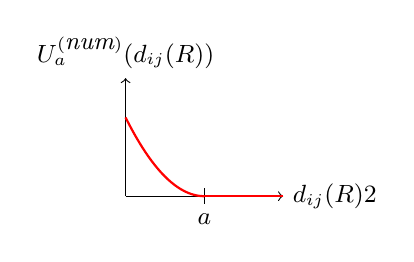
\begin{tikzpicture}
            \draw[->] (0,0) -- (2,0) node[right] {{\small $\dabs{d_{ij}(R)}{2}$}};
            \draw[->] (0,0) -- (0,1.5) node[above] {{\small $U_a^{(\textit{num})}(d_{ij}(R))$}};

            \draw[] (1,0.1) -- (1,-0.1) node[below] {{\small $a$}};
    
            \draw[thick, domain=0:1, smooth, variable=\x, red] plot ({\x}, {(\x - 1)^2});
            \draw[thick, domain=1:2, smooth, variable=\x, red] plot ({\x}, {0});
        \end{tikzpicture}
    }}
\]
Notice that for $a = 1$ we find the same form as \cite{Jacquin_2010}. To describe forces induced by the spring potential in $d$ dimensions in our system, we introduce radial symmetry by composing $f_a^{(\textit{num})}\circ\dabs{\cdot}{2}$ on any disctance $d_{ij}(R)$ of two particles $i,j$, i.e. we encode the isotropic character of the system into $f^{\textit{num}}_a$. With this we are now ready to calculate the particle probability density $R\mapsto {\exp}\bbra{-\beta\cdot U_a^{(\textit{num})}(R)}$ in the following.

        \subchapter{Analytical Methods}
        \cfoot{\textsc{Numerical Analysis: Analytical Methods}}

            \noindent
            The idea now is to reduce complexity of the model by using a mean field approach on the particle interaction potential $U_a^{(\textit{num})}$. This is done by untangling to direct and indirect contributions towards one specific particle $x$ in $R$ by seperation:\footnote{By $[2,N]$ we mean the set $\{2,\ldots,N\}$.}
\begin{align*}
    U_a^{(\textit{num})}(x,R_2,\ldots,R_N) = 2\cdot\sum_{j\in[2,N]}u_a(x - R_j) + \sum_{(i,j)\in[2,N]^2}u_a(R_i - R_j),
\end{align*}
and for two particles $x,y\in\R^d$ via 
\[
    U_a^{(\textit{num})}(x,y,R_3,\ldots,R_N) = 2\cdot\nbra{
        \sum_{j\in[3,N]}u_a(x - R_j) + u_a(y - R_j) + u_a(x - y)
    } + \sum_{(i,j)\in[3,N]^2}u_a(R_i - R_j)
\]
where the factor $2$ is a result of symmetry $u_a(x - y) = u_a(y - x)$ coming from the norm. The pair distribution function $g_N^{(2)}$ would then be given by 
\begin{multline*}
    g_N^{(2)}(x,R_2) \propto \int_{V_{d,N-2}}\prod_{j\in[N-2]}\exp(-\beta\cdot2\cdot\bbra{u_a(x - R_j) + u_a(R_2 - R_j) + u_a(x - R_2)})\\
    \cdot\prod_{(i,j)\in[N-2]^2}\exp(-\beta\cdot u_a(R_i - R_j))\;(\uplambda^d)^{N-2}(dR).
\end{multline*}
The radial distribution function $g_{\abs{}}(x,\dabs{R_2}{2})$ then can be calculated by integrating a radial sphere $B_{\dabs{R_2}{2}}(x)$ around the position $x$, which can be regarded as $0$ for large volumes.\footnote{Note that the accuracy of the approximation is depending on wether $0\in V_{d,N-2}$ and on the norm $\dabs{x}{2}$.} From this we get 
\[
    \R^d\ni R_2\mapsto g_0(R_2) = \int_{B_{\dabs{R_2}{2}}(0)}g_N^{(2)}(0,r)\;\uplambda^d(dr).
\]

\subsubchapter{Hypernetted Chain Approximation Method}
In general, for low densities $\rho_*\to 0$ the radial correlation function in a uniform fluid can be written explicitly using the Boltzmann density $\R^d\ni \vr\mapsto \exp(-\beta\cdot w(\vr))$ \cite[eq. 2.6.10]{book:HANSEN201313} for a pair potential $\R^d\ni R_i - R_j\mapsto w(R_i - R_j)$. Hereby $w$ is called the \emph{potential of mean force}. Uniformity further suggests $w$ to be radially symmetric. This can be founded on a diagrammatical reasoning on the iterative solution of the Ornstein-Zernike equation (introduced shortly in D.\ref{mdef:OrnsteinZernike}). The diagrams arise from the growing composition of integrals (see again \ref{mdef:OrnsteinZernike}) lead ultimately to a series expansion of the radial distribution function $g_{\textit{tot}}$ in terms of the density $\rho_*$ of the fluid \cite{book:HANSEN.chap4}. This expansion is given by
\[
    g_{\textit{tot}}(\vr) = \exp(-\beta\cdot w(\vr))\cdot\nbra{1 + \sum_{n = 1}^\infty\rho_*^n\cdot \tilde g_n(\vr)},
\]
where $\tilde g_n$ are coefficient functions of $g_{\textit{tot}}$'s expansion. From this we can immediately see our claim. Going forward, for higher order terms resulting from higher densities $\rho_*$ one needs to approximate the second factor. This is done by different approaches, known as \emph{closures}. We will take a look at the \emph{hypernetted chain approximation} (HNC) in the following.

% \color{red} CALLED POTENTIAL OF MEAN FORCE \color{black}
Since we in general do not know the mapping of $w$ we use an indirect approach. For this we make use of our radial potential $\R^d\ni \vr\mapsto u_a(\vr)$ by defining the \emph{direct} radial distribution function as $\R_{>0}\times\R^d\ni(a,\vr)\mapsto g_{\textit{dir}}(a,\vr) :\approx {\exp}\bbra{-\beta\cdot u_a(\vr)}$.\footnote{By $:\approx$ we mean that an approximation in the HNC was done here.} It makes the contribution of a direct interaction of our reference particle at position $\vr_{\textit{ref}} = 0$ with a particle in $\partial B_r(0)\subset\R^d$, i.e. an other particle at distance $r\in\R$, explicitly. Since there are more than two particles total to be assumed in the system, we provide the \emph{indirect} contribution to the radial distribution function as
\[
    g_{\textit{ind}}(a,\vr) := \exp(-\beta\cdot \bbra{w(\vr) - u_a(\vr)}),
\]
where we virtually subtract the already described direct part $u_a$ from the total potential $w$. This brings us to $g_{\textit{tot}}(a,\vr) = g_{\textit{ind}}(a,\vr) + g_{\textit{dir}}(a,\vr)$, which can be rearranged to
\[
    g_{\textit{dir}}(a,\vr) = \ubra{\exp(-\beta\cdot w(\vr))}{\text{total contribution }g_{\textit{tot}}(\vr)}  - \ubra{\exp(-\beta\cdot \bbra{w(\vr) - u_a(\vr)})}{\text{indirect contribution }g_{\textit{ind}}(r)}.
\]
% This can be visialized as a diagram in figure \ref{fig:DirectIndirectContribution}.
% \begin{figure}[H]
%     \centering
%     \begin{tikzpicture}
%         \draw[->] (0,0) -- ({2 * cos(30)},{2 * sin(30)}) node[left,above,midway] {$g_{\textit{dir}}$};
%         \draw[->] ({2 * cos(30)},{2 * sin(30)}) -- ({2 * cos(355)},{2 * sin(355)}) node[right,midway] {$g_{\textit{ind}}$};
% 
%         \draw[->] (0,0) -- ({2 * cos(355)},{2 * sin(355)}) node[below,midway] {$g_{\textit{tot}}$};
% 
%         \draw[fill=black] (0,0) circle (0.05) node[below] {$r_{\textit{ref}}$};
%         \draw[fill=black] ({2 * cos(30)},{2 * sin(30)}) circle (0.05) node[left,above] {$r$};
%         \draw[fill=red] ({2 * cos(355)},{2 * sin(355)}) circle (0.05);
%     \end{tikzpicture}
%     \caption{Direct and indirect contributions to the radial distribution function. Their sum is the total radial distribution function.}
%     \label{fig:DirectIndirectContribution}
% \end{figure}
\noindent Writing the series expansion of the exponential function we further find
\[
    g_{\textit{dir}}(a,\vr) = \exp(-\beta\cdot w(\vr))  - \Bbra{1 - \beta\cdot \bbra{w(\vr) - u_a(\vr)} + R_2(g_{\textit{ind}},0,\vr)}.
\]
Assuming that the contribution of the Taylor remainder $R_2(g_{\textit{ind}},0,\vr)$ is negligible and the difference $w(\vr) - u_a(\vr)$ is small\footnote{Again, where there would be a need of an error estimate, we do not make statements about the quality of the approximation in this work. Please take a look at \cite{book:HANSEN.chap3}.}, we can further simplify the expression to
\[
    g_{\textit{dir}}(a,\vr) = \ubra{g_{\textit{tot}}(a,\vr) - 1}{=:h(g_{\textit{tot}},a,\vr)} + \beta\cdot \bbra{w(\vr) - u_a(\vr)} \approx : c(g_{\textit{tot}},a,\vr).
\]
The newly defined function\footnote{Notice that in the definitions of $c$ and $h$ (as we have done in $g_{\textit{tot}}$, $g_{\textit{dir}}$ and $g_{\textit{ind}}$) we assume $\beta$ to be constant, otherwise we would write $c_\beta$ and $h_\beta$.} $c$ is known in literature as the \emph{direct correlation function}, while $h$ is called the \emph{pair correlation function} \cite{book:HANSEN.chap4}. Since the total potential $w$ is still unknown, we can express it using already occuring terms by its definition $w(\vr) = -\ln(g_{\textit{tot}}(a,\vr))/\beta$ to obtain a fixed point equation for $g_{\textit{tot}}$ using the \emph{Ornstein-Zernike equation}.
\begin{mdef}{Ornstein–Zernike equation}{OrnsteinZernike}
    For $g:\R^d\to\R$ at a fixed $\vr\in\R^d$ the Ornstein–Zernike equation on homogeneous densities $\R^d\ni r'\mapsto \rho(r') = \rho_*$ is given by
    \[
        h(g,r) = h(g,r) + \rho_*\cdot \int_{\R^d}c_a(g,r')\cdot h(g,r - r')\;\uplambda(dr') =: \Phi_{a,\rho_*,r}(g)
    \]
    Thereby $h:=g-1$ and $c(g,a,\vr) = g(\vr) - 1 + \beta\cdot (w(\vr) - u_a(\vr))$. If $\Phi_{a,\rho_*,r}$ is a contraction mapping, then $g$ is a solution of the Ornstein–Zernike equation.
\end{mdef}
    
The Ornstein-Zernike equation can now be used with the definition of $c$ to find the following hypernetted chain fixed point equation
\begin{align}
    \Phi_{a,r}:g_{\textit{tot}}\mapsto \ubra{c(g_{\textit{tot}},a,r)}{\text{direct}} + \ubra{\int_{\R}c(g_{\textit{tot}},a,r')\cdot \bbra{g_{\textit{tot}}(a,r - r') - 1}\;\uplambda(dr')}{\text{indirect}},\label{eq:FixedPointEquationHCA}\tag{HCA}
\end{align}
which is solved by $g_{\textit{tot}}$ as a zero of $g\mapsto \Phi_{a,r}(g) - g$, thus approaching the unknown potential function $w$ indirectly. Since we can again see a split of contributions to the indirect and direct part, the interpretation of the Ornstein Zernike equation becomes clear in the context of our earlier considerations.

\subsubchapter{Static Structure Factor}
If we successively find the fixed point $g_{\textit{tot}}$ of equation \eqref{eq:FixedPointEquationHCA} we can calculate the static structure factor $S_*$ from lemma \ref{mlem:StaticStructureFactorandRadialDistributionFunction} by
\begin{align}
    \R^d\ni \vq\mapsto S_*(\vq) = 1 + \rho_*\cdot\int_{\R^d}\exp(\cmath\cdot\scpr{\vq}{\vr})\cdot\bbra{g_{\textit{tot}}(a,\vr) - 1}\;\uplambda(d\vr). \label{eq:StaticStructureFactorHCA}\tag{SSF}
\end{align}
For simplicity we stick to a three dimensional space going forward. Since $w$ is radially symmetric, $\R^d\in \vr\mapsto g_{\textit{tot}}(a,\vr)$ also is a function changing with the vectors norm, i.e. in three dimensions radially symmetric. It turns out to be convenient to make a spherical coordinate transformation and considering $\R\ni r\mapsto g_{\abs{\text{tot}}}(a,r)$ going forward.\footnote{To recover dimensionality dependencies we write $w_\abs{}$ defined by $w(\vr) = (w_{\abs{}}\circ\dabs{\cdot}{2})(\vr)$ for $\vr\in\R^d$ and $r\mapsto g_{\abs{\text{tot}}}(r):=\exp(-\beta\cdot w_{\abs{}}(r))$, thus $g_{\textit{tot}}(\vr) = g_{\abs{\textit{tot}}}(\dabs{r}{2})$. The physicist will know that this is meant by radial symmetry of $g_{\textit{tot}}(\vr)$.} For this we use the cos relation $\cos(\vartheta)\cdot\dabs{\vq}{2}\cdot\dabs{\vr}{2} = \scpr{\vq}{\vr}$ based on the \emph{Cauchy-Schwarz Inequality} $\abs{\scpr{\cdot}{\cdot}}\leq\dabs{\cdot}{}\cdot\dabs{\cdot}{}$ for the scalar product of $\vq,\vr\in\R^3$ to transform the integral:
\[
    S_*(\vq) = 1 + \rho_*\cdot\int_{\R^3}\bbra{g_{\abs{\textit{tot}}}(a,\dabs{\vr}{2}) - 1}\cdot{\exp}\bbra{\cmath\cdot\dabs{\vq}{2}\cdot\dabs{\vr}{2}\cdot\cos(\vartheta)}\;\uplambda(dr).
\]
The spherical transformation function $(\rho,\vartheta,\varphi)\mapsto \rho\cdot (\sin(\vartheta)\cdot\cos(\varphi),\sin(\vartheta)\cdot\sin(\varphi),\cos(\vartheta))$ yields a Jacobian determinant of $(\rho,\vartheta)\mapsto \rho^2\cdot\sin(\vartheta)$, which represents our integral in spherical coordinates as
\[
    \int_{(-\pi,\pi)}\int_{\R_{>0}}\int_{[0,\pi)}\nsqbra{\bbra{g_{\abs{\textit{tot}}}(a,\rho) - 1}\cdot\exp(\cmath\cdot\rho\cdot\dabs{\vq}{2}\cdot\cos(\vartheta))}\cdot\rho^2\cdot\sin(\vartheta)\;\uplambda^3(d(\vartheta,\rho,\varphi)).
\]
Evaluation of the outer integral to $2\pi$ can be done effortlessly since there appears no dependency on $\varphi$. The factor $(g_0(\rho) - 1)$ can be linearly interchanged with $\int_{[0,\pi)}$ such that the inner integral is performed on 
\[
    \R\ni\vartheta\mapsto \sin(\vartheta)\cdot{\exp}\bbra{\cmath\cdot\rho\cdot\dabs{\vq}{2}\cdot\cos(\vartheta)}.
\]
Noticing the cos function in the exponential we can use the chain rule of differentiation to find 
\[
    \sin(\vartheta)\cdot{\exp}\bbra{\cmath\cdot\rho\cdot\dabs{\vq}{2}\cdot\cos(\vartheta)} = -\bbra{\cmath\cdot\rho\cdot\dabs{\vq}{2}}^{-1}\cdot\frac{d}{d\vartheta}\,{\exp}\bbra{\cmath\cdot\rho\cdot\dabs{\vq}{2}\cdot\cos(\vartheta)}
\]
for given $\rho\in\R_{>0}$ and $\vq\in\R^3$. The differentiation means vanishing integration with respect to $\vartheta$, such that evaluation yields
\[
    \R\times\R^3\ni(\rho,\vq)\mapsto \frac{\cmath}{\dabs{\vq}{2}\cdot\rho}\cdot\Bbra{
        {\exp}\bbra{-\cmath\cdot \dabs{\vq}{2}\cdot\rho} - {\exp}\bbra{\cmath\cdot \dabs{\vq}{2}\cdot\rho}
    }.
\]
This basically is the definition of sinc, since $\sin(x) = (e^{\cmath x} - e^{-\cmath x})/(2\cdot\cmath)$ and $\sinc(x) = \sin(x)/x$, such that the mapping is eqivalent to $(\rho,q)\mapsto 2\cdot\sinc(\dabs{\vq}{2}\cdot\rho)$.
As a result the integration over $\R^3$ turns out to be an integration over $\R_{>0}$ with respect to $\rho$ at given wave vectors $\vq\in\R^3$ of the \underline{I}ntegrand of the static \underline{S}tructure factor relation in \underline{S}pherical coordinates\footnote{Pun intended.}
\begin{align}
    \rho\mapsto 4\pi\cdot\bbra{g_{\textit{tot}}(a,\rho) - 1}\cdot\rho^2\cdot\sinc(\dabs{\vq}{2}\cdot\rho)
    \label{eq:IntegrandSstarPolar}\tag{ISS}
\end{align}
Notice that the vector arguments $\vq$ in no form utilize their directional components, such that the integrand is a radial symmetric function of $\R_{\neq 0}\ni q\mapsto S_{\abs{*}}(q)$. Coming back to equation \eqref{eq:StaticStructureFactorHCA} we can now evaluate the integral over $\R_{>0}$ to define a radially symmetric static structure factor $\R_{\neq 0}\ni q\mapsto S_*(q)$ as
\[
    S_*(\vq) = 1 + 4\pi\cdot\rho_*\cdot\int_{\R_{>0}}\bbra{g_{\abs{\textit{tot}}}(a,\rho) - 1}\cdot \rho^2\cdot\sinc(\dabs{\vq}{2}\cdot\rho)\;\uplambda(d\rho).
\]


\subsubchapter{Dyson Equation Fixed Point Form}
The last step now to be taken is to find the fixed point of the Dyson equation in first loop order. 

% \begin{mlem}{Fourier Transform of Heaviside Function}{FourierTransformOfHeaviside}
    Let $H_a:\R\to\R$ be for $a\in\R$ defined by 
    \[
        H_a(x) := \begin{cases}
            1 & \text{if } x < a, \\
            0 & \text{if } x > a.
        \end{cases}
    \]
    Then the Fourier transform of $H_a$ is given by
    \[
        \R\ni\omega\mapsto\hat H_a(\omega) = \exp(\cmath\cdot a\cdot \omega)\cdot\frac{1}{\cmath\cdot\omega} + \pi\cdot\delta_0(\omega).
    \]
\end{mlem}  
\begin{mlem}{Fourier Transform of Heaviside-Based Spring Function}{FourierTransformOfHeavisideSpring}
    Let $H_a:\R\to\R$ for $a\in\R_{>0}$ be the Heaviside function defined as
    \[
        H_a(x) := \begin{cases}
            1 & \text{if } x<a, \\
            0 & \text{else}.
        \end{cases} = \mbbEins_{[0,a)}(x).
    \]
    Then for $3$ dimensional arguments $\vr\in\R^3$ the Fourier transform of $F_a(\vr):=H_a\bbra{\dabs{\vr}{2}}$ is given by 
    \[
        \R^3\ni\vq\mapsto \hat F_a(\vq) = 4\pi\cdot\bbra{\sin(a\cdot\dabs{\vq}{2}) - a\cdot\dabs{\vq}{2}\cdot\cos(a\cdot\dabs{\vq}{2})}\cdot\dabs{\vq}{2}^{-3}.
    \]
    Furthermore it has a removable singularity at $\vq = 0$ with $(\mcF F_a)(\mathbf{0}) = 4\pi a^3/3$. From its radial symmetry the existence of $\hat F_{a,\abs{}}:\R\to\R$ with $\hat F_a = \hat F_{a,\abs{}}\circ\dabs{\cdot}{2}$ follows. 
\end{mlem}
The proof is given in the Appendix. With this we can define the bare propagator $\R^3\times\C\ni(\vp,z)\mapsto G_0(\vp,z)$ and the Vertex function $(\R^3)^2\ni(\vq,\vp)\mapsto V(\vq,\vp)$ both are needed for the self energy $\R^3\times\C\ni(\vp,z)\mapsto \Sigma^{(1)}(\vp,z)$. The first function is given by
\[
    \R^3\times\C\ni(\vp,z)\mapsto G_0(\vp,z) = \frac{1}{z - \rho_*\cdot\bbra{\hat F_a(\mathbf{0}) - \hat F_a(\vp)}},
\]
whereas the vertex function is given by 
\[
    \R^2\ni (\vq,\vp)\mapsto V(\vq,\vp) = \rho_*\cdot\bbra{\hat F_a(\vq) - \hat F_a(\vq - \vp)}.
\]
From this we are already able to build up the integral representation which we will use as our fixed point iteration for the propagator $(\vp,z)\mapsto G(\vp,z)$ in the first loop order. It is firstly of the form 
\[
    G\mapsto \frac{G_0(\vp,z)^2}{\rho_*}\cdot\int_{\R^3}S_*(\vq)\cdot G(\vp - \vq,z)\cdot V(\vq,\vp)^2\;\uplambdabar(d\vq),
\]
where we again need to spherically deal with the three dimensional integral. But before we do so, since our goal is numerical analysis, we will have to discretize the integral later on. Since we need to iterate over discrete evaluations of $G$ at gridpoints $\vq_i$, we transform the integral linearely with $\vq\mapsto \vp - \vq$ to get
\[
    G\mapsto G_0(\vp,z) \cdot \nbra{1 + \frac{G_0(\vp,z)}{\rho_*}\cdot\int_{\R^3}S_*(\vp - \vq)\cdot G(\vq,z)\cdot V(\vp - \vq,\vp)^2\;\uplambdabar(d\vq)}^{-1}.
\]
Conveniently we have proven a symmetry in $V$ during its introduction in TD.\ref{msatdef:VertexFunction}, which unveils a simplification $\bbra{V(\vp - \vq,\vp)}^2 = (-1)^2\cdot\bbra{-V(\vp - \vq,\vp)}^2 = V(\vq,\vp)^2$. Lastly using D.\ref{mdef:DysonFixpoint} and the geometric series by preassuming $\int_{\R^3}S_*(\vp - \vq)\cdot G(\vq,z)\cdot V(\vq,\vp)^2\;\uplambdabar(d\vq)\cdot G_0(\vp,z)^2/\rho_*\in [0,1)$ the fixed point form convertes to 
\[
    G\mapsto \nbra{G_0(\vp,z)^{-1} - \rho_*^{-1}\cdot\int_{\R^3}S_*(\vp - \vq)\cdot G(\vq,z)\cdot V(\vq,\vp)^2\;\uplambdabar(d\vq)}^{-1}.
\]
Later on we can use a matrix representation for the integral of the form $\text{IntM}\cdot G_v$ due to the grid $Q = \{q_1,\ldots,q_{n_q}\}$. But before doing so we continue the analytic discussion.
Performing the spherical transformation by again using $\Phi:(\rho,\vartheta,\varphi)\mapsto \rho\cdot (\sin(\vartheta)\cdot\cos(\varphi),\sin(\vartheta)\cdot\sin(\varphi),\cos(\vartheta))$ we get
\[
    \int_{(-\pi,\pi)}\int_{\R_{>0}}\int_{[0,\pi)}\nsqbra{S_*\bbra{\vp - \Phi(\vartheta,\rho,\varphi)}\cdot G_{\abs{}}(\rho,z)\cdot V\bbra{\Phi(\vartheta,\rho,\varphi),\vp}^2}\cdot\rho^2\cdot\sin(\vartheta)\;\uplambda^3(d(\vartheta,\rho,\varphi)).
\]
It was easy to replace $\vq$ with $\rho$ within $G_{\abs{}}$ since we directly have $G_0 = G_{\abs{0}}\circ\dabs{\cdot}{2}$ from $\hat F_a = \hat F_{a,\abs{}}\circ\dabs{}{2}$ for scalar Functions $G_{\abs{0}}$ and $F_{a,\abs{}}$, see L.\ref{mlem:FourierTransformOfHeavisideSpring}. Following the iteration of the fixed point equation, this radial symmetry is reserved for all following propagators.

For the other functions we have to be more careful. With $\vp\in\R^3$ we have
\[
    \dabs{\vp - \Phi(\vartheta,\rho,\varphi)}{2}^2 = \dabs{\vp}{2}^2 + \rho^2 - 2\cdot\scpr{\vp}{\Phi(\vartheta,\rho,\varphi)},
\]
where $\dabs{\Phi(\vartheta,\rho,\varphi)}{2} = \rho$. From the radial symmetry in $\vp$ we can freely choose the particular direction of $\vp$. Looking at the spherical transformation $\Phi$ we decide on $\vp = \dabs{\vp}{2}\cdot e_3$ such that
\[
    \scpr{\vp}{\Phi(\vartheta,\rho,\varphi)} = \dabs{\vp}{2}\cdot\cos(\vartheta)\cdot\rho.
\]
Furthermore the norm is now accessible by only $\rho$, $\vartheta$ and $\dabs{\vp}{2}$, such that a scalar function can be used:
\[
    \dabs{\vp - \Phi(\vartheta,\rho,\varphi)}{2}^2 \stackrel{\vp = p\cdot e_3}{=} p^2 + \rho^2 - 2\cdot p\cdot\rho\cdot\cos(\vartheta) =: N(p,\rho,\vartheta).
\]
Defining $\R^2\ni(x,y)\mapsto V_{\abs{}}(x,x-y):=\rho_*\cdot\bbra{\hat F_{a,\abs{}}(x) - \hat F_{a,\abs{}}(x-y)}$ we hereby get the integrand
\begin{align}
    (p,\vartheta,\rho)\mapsto
    S_{\abs{*}}\bbra{
            N(p,\rho,\vartheta)
        }\cdot G_{\abs{}}(\rho,z)\cdot V_{\abs{}}(\rho,N(p,\rho,\vartheta))^2
    \cdot\rho^2\cdot\sin(\vartheta). \label{eq:IntegrandFixedPointDysonTransformed}
\end{align}
Since we can already see the independence of $\varphi$ due to the direction of $\vp$ the integral $\int_{(-\pi,\pi)}\ldots\;\uplambda(d\varphi)$ is easily evaluated to $2\pi$. Setting $\text{Int}(\vp,\vartheta,\rho):=2\pi\cdot\eqref{eq:IntegrandFixedPointDysonTransformed}$ we can now formulate the fixed point equation based on the dyson formalism that is used in the following numerical analysis for arguments $(p,z)\in\R\times\C$ as
\begin{align}
    G\mapsto \nbra{
        z - \rho_*\cdot\bbra{\hat F_{a,\abs{}}(0) - \hat F_{a,\abs{}}(p)} - (\rho_*)^{-1}\cdot\int_{\R_{>0}}\int_{[0,\pi)}\text{Int}(\vp,\vartheta,\rho)\;\uplambda^2(d(\vartheta,\rho))
    }^{-1}. \label{eq:FixedPointEquationDysonTransformed}\tag{DF}
\end{align}
Now the question of implementation remains to be discussed.


        \subchapter{Numerical Methods}
        \cfoot{\textsc{Numerical Analysis: Numerical Methods}}
        
            \noindent
            For the implementation we decide to use the programming language \href{https://julialang.org/}{Julia} for its high performance, flexibility and the ability to write code that is close to mathematical notation. Our implementation therefore requires the following packages:
\begin{mdframed}[backgroundcolor=black!4, topline=false, bottomline=false, rightline=false, leftline=false]
    \begin{lstlisting}[language=Julia,basicstyle=\small]
using Distributed
using OrnsteinZernike, GLMakie, FFTW, Statistics, ProgressMeter, QuadGK, NLsolve, ForwardDiff, LinearAlgebra, LoopVectorization, Base.Threads, CSV, DataFrames
    \end{lstlisting}
\end{mdframed}

To get the basics out of the way, for $d = 3$ and $kBT = 1$ we define on the parameter tuple $p = (1.0, 2.0, 1.0)$ the spring function $f$ and the potential $U_{\textit{neu}}$ as 
\begin{mdframed}[backgroundcolor=black!4, topline=false, bottomline=false, rightline=false, leftline=false]
    \begin{lstlisting}[language=Julia,basicstyle=\small]
@everywhere function HeavisideSpring(r,p)
    if r < p[3]
        return 1
    else
        return 0
    end
end
    
@everywhere function U_HeavisideSpring(r, p)
    if r < p[3]
        return 0.5 * (r - p[1])^p[2]
    else
        return 0
    end
end
    \end{lstlisting}
\end{mdframed}
The @everywhere macro is used in Julia for distributed computing.

\subsubsection*{Numerical HNC Approximation}

The implementation of the hypernetted chain fixed point equation from \eqref{eq:FixedPointEquationHCA} turns out to be tricky, since our fixpoint essentially needs to be a function of $r\in\R$. It is also needed to evaluate a folding with $r'\mapsto g_{\textit{tot}}(r - r')-1$. For a fixed $a\in\R$ the implementation can be done via
\begin{mdframed}[backgroundcolor=black!4, topline=false, bottomline=false, rightline=false, leftline=false]
    \begin{lstlisting}[language=Julia,basicstyle=\small]
g_hca = r -> exp(-β * U_num(r))
c_hca = (g, r) -> g(r) - 1 - log(g(r)) - β * U_num(r)
int_hca = (g, r) -> hcubature(
    rs -> c_hca(g, rs) * (g_hca(r - rs) - 1),
    [vol_min for dim in 1:length(r)],
    [vol_max for dim in 1:length(r)],
    rtol=1e-5
)[1]
Φ_hca = g -> r -> c_hca(g, r) + int_hca(g, r)
    \end{lstlisting}
\end{mdframed}
and a following iteration over $g$, which in our testing turned out to converge very slowly. Instead we will use the work of Ilian Pihlajamaa on his GitHub repository \href{https://github.com/IlianPihlajamaa/OrnsteinZernike.jl}{IlianPihlajamaa/OrnsteinZernike.jl} for a more efficient implementation and straightforward implementation.\footnote{Again, I want to express my gratitude to Ilian Pihlajamaa for his amazing work on this package.}


\begin{mdframed}[backgroundcolor=black!4, topline=false, bottomline=false, rightline=false, leftline=false]
    \begin{lstlisting}[language=Julia,basicstyle=\small]
# -> Define system potential (model)
potential = CustomPotential(Uf, params)

# -> Create System struct
system = SimpleLiquid(d, ρ, kBT, potential)

# -> Define solving closure
closure = HypernettedChain()

# -> generate solution from system parameters
solution = @time solve(system, closure)
    \end{lstlisting}
\end{mdframed}
This yields a solution object with \texttt{solution.r} as the radii that $g$ has been evaluated on and \texttt{solution.gr} as the corresponding values of $g$. For the first we also use the Symbol $G_r$ to denote the grid points of $r$.



\subsubsection*{Numerical Structure Factor}
Now we are ready to discretize the integral $\int_{\R_{>0}}$ on $[0,R]$ for $R>0$ given by $R = \max(G_r)$ with respect to $\rho$ as
\[
    \int_{[0,R]}\eqref{eq:IntegrandSstarPolar}\; d\rho \approx \sum_{\rho\in G_r}4\pi\cdot\bbra{g(\rho) - 1}\cdot\rho^2\cdot\sinc(\rho\cdot q)
    \cdot\Delta\rho.
\]
By default we work with a grid resolution of $1024$ points. To test and enhance convergence this is altered but not explicitly mentioned in the following. The discretized integral can now be implemented via
\begin{mdframed}[backgroundcolor=black!4, topline=false, bottomline=false, rightline=false, leftline=false]
    \begin{lstlisting}[language=Julia,basicstyle=\small]
cFT_integrand = (q,r) -> 2 * sinc(q * r)
cFT = q -> begin
	if exp_g_toggle
		sum(r^2 * 2 * pi * (exp(-1 * Uf(r, params)) - 1) * x * Δr for (x,r) in zip(cFT_integrand.(q, solution.r),solution.r))
	else 
		sum([r^2 * 2 * pi * gm * x * Δr for (x,gm,r) in zip(cFT_integrand.(q, solution.r),[x - 1 for x in solution.gr],solution.r)]) # use cFT_integrand on all r values from solution.r, then discretely integr.
	end
end
    \end{lstlisting}
\end{mdframed}
Hereby exp\_g\_toggle is a boolean that switches between the Heaviside and the exponential spring function later on.
To finally calculate the static structure factor, which now also has radial symmetry $\R\ni\vq\mapsto S_*(q)$, we simply take the real part of $q\mapsto \text{cFT}(q)$ with the following code
\begin{mdframed}[backgroundcolor=black!4, topline=false, bottomline=false, rightline=false, leftline=false]
    \begin{lstlisting}[language=Julia,basicstyle=\small]
S_k = q -> 1 + ρ * real(cFT(q))
    \end{lstlisting}
\end{mdframed}


\subsubsection*{Numerical Dyson Fixed Point Equation}
For the numerical structure factor we need to calculate the fourier transformed spring function $\hat F_a$ from L.\ref{mlem:FourierTransformOfHeavisideSpring}. Plotting in one dimension gives us the graph shown in Figure \ref{fig:FourierTransformSpringFunction}. Notice that $\hat F_1$ has its maximum at $\omega = 0$ and decays to $0$ for $\omega\to\infty$. 
\begin{figure}[H]
    \centering
    \begin{tikzpicture}
        \clip (-0.5,-0.5) rectangle (10.5,3);

        \draw[->] (0.1,0) -- (10,0) node[right] {$\omega$};
        \draw[->] (0.1,0) -- (0.1,2.5) node[above] {$\hat F_1(\omega)$};

        \draw[] (0,4.18) -- (0.1,4.18) node[left] {$\frac{4\pi}{3}$};

        \draw[YvesKlein, samples=1000, domain=0.1:10] plot (\x, {2 * 3.141592 * (sin(\x r) - \x * cos(\x r))/(\x^3)});
        % \draw[YvesKlein, samples=20, domain=0:0.15] plot (\x, {2 * 3.141592 * (4/3 - 2*\x^2/15 + \x^4/105)});
    \end{tikzpicture}
    \caption{Graphical representation of the Fourier transform $\hat F_1$ of the Heaviside spring function $F_1:=H_a\circ\dabs{\cdot}{2}$ in three dimensions. The argument domain is $\omega\in[0,10]$.}
    \label{fig:FourierTransformSpringFunction}
\end{figure}
\noindent Since around $\omega = 0$ the function has a removable singularity, for numerical stability it \emph{can} be helpful to use an approximation of $\hat F_a$ using its Taylor expansion for small $\omega$ as
\[
    \hat F_a(\dabs{\vq}{2}) = \frac{4 \pi a^{3}}{3} - \frac{2 \pi a^{5} \dabs{\vq}{2}^{2}}{15} + \frac{\pi a^{7} \dabs{\vq}{2}^{4}}{210} + \mcO\bbra{\dabs{\vq}{2}^6}.
\]
However it does not guarantee better results, as our numerical tests have shown. Nevertheless its implementation in Julia reads
\begin{mdframed}[backgroundcolor=black!4, topline=false, bottomline=false, rightline=false, leftline=false]
    \begin{lstlisting}[language=Julia,basicstyle=\small]
@everywhere function FHeavisideSpring_1d(ω)
    local p = params

    if ω == 0.0
        return 4 * pi * p[3]^3/3
    # elseif ω < 0.01
        # return ((4*pi)/(3))-((2*ω^(2)*pi)/(15))+((ω^(4)*pi)/(210))-((ω^(6)*pi)/(11340))+((ω^(8)*pi)/(997920))-((ω^(10)*pi)/(129729600));
    else
        return 4 * pi * (sin(p[3] * ω) - p[3] * ω * cos(p[3] * ω)) * ω^(-3)
    end
end
    \end{lstlisting}
\end{mdframed}
The integral found for the Dyson fixed point equation in \eqref{eq:FixedPointEquationDysonTransformed} now needs to be discretized and implemented. Herefor we choose a grid $Q = \{q_1,\ldots,q_{n_q}\}$ with $q_1 = \epsilon$ and $q_{n_q} = q_{\text{max}} - \Delta q$, with equal spacing to begin with. The maximum value $q_{\text{max}}$ is set to $30$, but also altered later on due to numerical instabilities in some regions. For the domain of angles we choose $\{\vartheta_1,\ldots,\vartheta_{n_\vartheta}\}$ with $\vartheta_1 = 0$ and $\vartheta_{n_\vartheta} = \pi - \Delta\vartheta$ with equal spacing $\Delta\vartheta = \pi/n_\vartheta$. This lets us approximate the integrand as
\[
    I:p\mapsto S_{\abs{*}}\Bbra{\sqrt{p^2 + q_i^2 - 2\cdot p\cdot q_j\cdot\cos(\vartheta_k)}}\cdot V_{\abs{}}\Bbra{\sqrt{q_i,p^2 + q_i^2 - 2\cdot p\cdot q_i\cdot\cos(\vartheta_i)}}^2\cdot q_i^2\cdot\sin(\vartheta_i).
\] 
The integration now includes the widths $\Delta q$ and $\Delta\vartheta$. All together, we have
\[
    \int_{\R_{>0}}\int_{[0,\pi)}\eqref{eq:FixedPointEquationDysonTransformed}\; d\vartheta d\rho \approx \sum_{q\in Q}\sum_{\vartheta\in\Theta} I_{q,\vartheta}(p)\cdot\Delta q\cdot\Delta\vartheta.
\]
Notice now that $(p,q)\mapsto I_{q,\vartheta}(p)$ on gridpoints $Q$ will yield a matrix of sums over angles, which can be used to represent the integration. Defining $\text{IntM}(i,j):=I_{q_i,\cdot}(q_j)$ we can write the integral as
\[
    \int_{\R_{>0}}\int_{[0,\pi)}\eqref{eq:FixedPointEquationDysonTransformed}\; d\vartheta d\rho \approx\text{IntM}\cdot G_v,
\] 
Where $G_v := \fdef{G(q_i,z)}{i\in[n_q]}$ is the discrete propagator vector. The implementation of this idea reads:
\begin{mdframed}[backgroundcolor=black!4, topline=false, bottomline=false, rightline=false, leftline=false]
    \begin{lstlisting}[language=Julia,basicstyle=\small]
BarePropagator = (ω,z) -> 1 / (z - ρ * (Ff(0) - Ff(ω)))
Vertex = (x,y) -> (Ff(x) - Ff(y))

Integrand = Gv -> (p, q, θ) -> begin
    norm_val = NormPminusSph_safe(p, q, θ)
    if norm_val <= 0
        throw(ArgumentError("Norm value is negative at p = $p, r = $q, θ = $θ"))
    end
    if structure_factor_toggle
    	return S_safe(norm_val) * Vertex(q,norm_val)^2 * q^2 * sin(θ) * (2 * pi)^(-2)
	else 
		return 1 * Vertex(q,norm_val)^2 * q^2 * sin(θ) * (2 * pi)^(-2)
	end
end

# -> Build Integration matrix
IntegrationMatrix = zeros(length(Q), length(Q))

# -> Fill Integration matrix
@time @showprogress @threads for i in 1:length(Q)
	p = Q[i]
	for j in 1:length(Q)
		q = Q[j]
		if j == 1
			IntegrationMatrix[j,i] = sum(Integrand(Gv)(p,q,θ) * Δθ for θ in θRange)
		else 
			IntegrationMatrix[j,i] = sum(Integrand(Gv)(p,q,θ) * Δθ for θ in θRange) * (Q[j] - Q[j-1])
		end
	end
end
    \end{lstlisting}
\end{mdframed}
Hereby the norm function $N(p,\rho,\vartheta)$ is implemented accordingly, while avoiding division by zero:
\begin{mdframed}[backgroundcolor=black!4, topline=false, bottomline=false, rightline=false, leftline=false]
    \begin{lstlisting}[language=Julia,basicstyle=\small]
NormPminusSph_safe = (p,r,θ) -> begin
	norm_val = (p^2 + r^2 - 2 * p * r * cos(θ))^0.5
	if norm_val <= 0
		norm_val = eps()
	end
	return norm_val
end
    \end{lstlisting}
\end{mdframed}
The iteration now is done over the propagator definition, where 
\[
    G_v(i)\mapsto \frac{1}{
        z - \rho\cdot\bbra{\hat F_1(0) - \hat F_1(q)} - \rho^{-1}\cdot(\text{IntM}\cdot G_v)_i
    }
\]
states the value of $G$ at a gridpoint $q_i$. 
\begin{mdframed}[backgroundcolor=black!4, topline=false, bottomline=false, rightline=false, leftline=false]
    \begin{lstlisting}[language=Julia,basicstyle=\small]
MDiscreteOneLoopSelfEnergy = Gv -> (IntegrationMatrix * Gv)

# -> Define Iterator function
MIterator = Gv -> [(z - ρ * (Ff(0) - Ff(p)) - ρ * MDiscreteOneLoopSelfEnergy(Gv)[i])^(-1) for (i,p) in enumerate(Q)]
    \end{lstlisting}
\end{mdframed}
The iteration is done using the package \href{https://github.com/JuliaNLSolvers/NLsolve.jl}{\texttt{NLsolve}} in Julia, such that the following code can be used:
\begin{mdframed}[backgroundcolor=black!4, topline=false, bottomline=false, rightline=false, leftline=false]
    \begin{lstlisting}[language=Julia,basicstyle=\small]
z = 0.0
initial_Gv = Gv(0.0)

result = @time fixedpoint(x -> MIterator(x), initial_Gv, show_trace = true, ftol=1e-2, iterations = iterations_count)
    \end{lstlisting}
\end{mdframed}

For small densities $\rho_*$ an other approximation can be done, by changing the radial distribution function from its definition to an exponential ansatz defined by $g_{\mathit{exp}}:\vr\mapsto \exp(-u_a(\vr)) = \exp(-(\dabs{\vr}{2} - a)^2/2)$, which essentially is stated by our potential $u_a(r)$ that resulted in the chapters introduction from the spring function $f_a^{(\textit{num})}$. \\

Another ansatz is a gaussian spring function $f^{(\textit{gauß})}:r\mapsto \exp(-r^2/2)$. For its implementation the Fourier transformed spring function in three dimensions is needed. Since the integral at hand yields
\begin{align*}
    \bbra{\mcF (f^{(\textit{gauß})}\circ\dabs{\cdot}{2})}(\vq) &= 2\pi\cdot\int_{\R_>0}\int_{[0,\pi)}\exp(\frac{-\rho^2}{2})\cdot\rho^2\cdot\sin(\vartheta)\cdot\exp(\cmath\cdot\rho\cdot \dabs{\vq}{2}\cdot\cos(\vartheta))\;\uplambda(d\vartheta)\;\uplambda(d\rho) \\
    &= 4\pi\cdot\int_{\R_{>0}}\exp(\frac{-\rho^2}{2})\cdot\rho^2\cdot\sinc(\rho\cdot \dabs{\vq}{2})\;\uplambda(d\rho), \numberthis\label{eq:FourierGaussian}
\end{align*}
only the generated potential function is left to be evaluated. For it there are two integrations needed:\footnote{The result can be verified by using a symbolic computation software like \href{https://www.wolframalpha.com/}{Wolfram Alpha}. One can use the input \texttt{Integrate[Integrate[exp(-x\textasciicircum 2/2),$\{$x,0,y$\}$],$\{$y,0,t$\}$]}. As we do not discuss this model in this thesis, we will not give further proof.}
\[
    U^{(\textit{gauß})}(r) = \int_{(0,r)}\int_{(0,\rho)}\exp(-\frac{\xi^2}{2})\;\uplambda(d\xi)\;\uplambda(d\rho) = \sqrt{\frac{\pi}{2}}\cdot r\cdot\text{erf}\nbra{\frac{r}{\sqrt{2}}} + \exp(-\frac{r^2}{2}) - 1.
\]
Hereby $\text{erf}(x):= \frac{2}{\sqrt{\pi}}\int_{0}^{x}\exp(-t^2)\;dt$ is the error function. Although the principal implementation is straightforward, we encountered numerical errors while evaluation within our time constraints, such that this model cannot be discussed in this thesis. \\

        \subchapter{Numerical Results}
        \cfoot{\textsc{Numerical Analysis: Numerical Results}}
        
            \noindent
            Using the approximations and techniques discussed in the previous sections we were able to make several observations. To begin with, the \emph{radial distribution function} for our system, which is given by a quadratic pair potential function $r\mapsto 0.5\cdot(r - 1)^2$ resulting from the chosen spring function, has the predicted course and does converge to $1$, as one can see in Figure \ref{fig:RadialDistributionFunctionMultDens}.

\begin{figure}[H]
    \centering
    \begin{tikzpicture}
        \begin{axis}[
            axis x line=bottom,
            axis y line=left,
            xlabel={$\dabs{\vr}{2}$},
            ylabel={$g_0(\vr)$},
            grid=both,
            grid style={line width=.1pt, draw=gray!10},
            major grid style={line width=.2pt,draw=gray!50},
            xmax=4,
            ymax=1.1,
            minor tick num=4,
            width=0.8\textwidth,
            height=0.4\textwidth,
            legend pos=east,
            legend style={
                at={(1.1,0.5)}, % Position innerhalb der Achse (rechts Mitte)
                anchor=west,    % Ankerpunkt auf der rechten Seite
                column sep=1ex, % Abstand zwischen den Legenden-Einträgen
            }
        ]
        % \addplot[color=YvesKlein] table[col sep=comma, x=r, y=gr] {Inhalt/Numerik/TestOZ/1.5-100-nS-Ur.csv};

        \addplot[color=twopointzero] table[col sep=comma, x=k, y=gr] {Inhalt/Numerik/Data-Cor-S/0.2-512-20-S-Heaviside.csv};
        \addlegendentry{$\rho_* = 0.2$}

        \addplot[color = fivepointzero] table[col sep=comma, x=k, y=gr] {Inhalt/Numerik/Data/1.0-1024.csv};
        \addlegendentry{$\rho_* = 1.0$}

        \addplot[color=tenpointzero] table[col sep=comma, x=k, y=gr] {Inhalt/Numerik/Data/2.0-1024.csv};
        \addlegendentry{$\rho_* = 2.0$}

        \addplot[color=twentypointzero] table[col sep=comma, x=k, y=gr] {Inhalt/Numerik/Data-with-S/5.0-1024-S.csv};
        \addlegendentry{$\rho_* = 5.0$}

        \addplot[color=fiftypointzero] table[col sep=comma, x=k, y=gr] {Inhalt/Numerik/Data-with-S/8.0-1024-20-S.csv};
        \addlegendentry{$\rho_* = 8.0$}

        \addplot[color=twohundredpointzero] table[col sep=comma, x=k, y=gr] {Inhalt/Numerik/Data-with-S/10.0-1024-20-S.csv};
        \addlegendentry{$\rho_* = 10.0$}

        \end{axis}
    \end{tikzpicture}
    \caption{The radial distribution function $\vr\mapsto g_0(\vr) = g_\abs(0,\dabs{\vr}{2})$ on a general scale.}
    \label{fig:RadialDistributionFunctionMultDens}
\end{figure}
It gives, as we have seen in previous chapters, a measure of the probability of finding a particle at a distance $r\in\R_{>0}$ from another particle. Having a maximum at $2$ is by construction of the potential and hard-coded into the spring function, since we can interpret the scalar $a$ as a particle diameter. In a general course one also notices, that the starting amplitude near $\dabs{\vr}{2} = 0$ increases with density $\rho_*$. Since we have a soft sphere model at hand, overlapping of particles is not \emph{forbidden} but rather restricted by the potential function. For growing densities however, it comes natural that particle overlap is more likely. The convergence to $1$ furthermore suggests, that for large distances the information about particle probability is lost and therefore finalizes in a uniform distribution. 

One can also directly observe a small shift and increase in the maximum of the radial distribution function $g_0$ as the density $\rho_*$ increases. This can be seen when zooming in on the maximum of the function, as shown in Figure \ref{fig:RadialDistributionFunctionMultDensZoomed}. Notice that we do not see a region of $g_0$ being nearly zero for small radii, as it was the case in our example in figure \ref{fig:RadialDensityFunction}. This clearly is expected, since we use a different potential function here. A similar form to the previous example would be gained by using the Lennard-Jones potential.
\begin{figure}[H]
    \centering
    \begin{tikzpicture}
        \begin{axis}[
            axis x line=bottom,
            axis y line=left,
            xlabel={$\dabs{\mathbf{r}}{2}$},
            ylabel={$g_0(\vr)$},
            grid=both,
            grid style={line width=.1pt, draw=gray!10},
            major grid style={line width=.2pt,draw=gray!50},
            minor tick num=4,
            xmin=1.5,
            xmax=2.5,
            ymin=0.98,
            ymax=1.01,
            width=0.8\textwidth,
            height=0.4\textwidth,
            legend pos=east,
            legend style={
                at={(1.1,0.5)}, % Position innerhalb der Achse (rechts Mitte)
                anchor=west,    % Ankerpunkt auf der rechten Seite
                column sep=1ex, % Abstand zwischen den Legenden-Einträgen
            }
        ]
        % \addplot[color=YvesKlein] table[col sep=comma, x=r, y=gr] {Inhalt/Numerik/TestOZ/1.5-100-nS-Ur.csv};

        \addplot[color=twopointzero] table[col sep=comma, x=k, y=gr] {Inhalt/Numerik/Data-Cor-S/0.2-512-20-S-Heaviside.csv};
        \addlegendentry{$\rho_* = 0.2$}

        \addplot[color = fivepointzero] table[col sep=comma, x=k, y=gr] {Inhalt/Numerik/Data/1.0-1024.csv};
        \addlegendentry{$\rho_* = 1.0$}

        \addplot[color=tenpointzero] table[col sep=comma, x=k, y=gr] {Inhalt/Numerik/Data/2.0-1024.csv};
        \addlegendentry{$\rho_* = 2.0$}

        \addplot[color=twentypointzero] table[col sep=comma, x=k, y=gr] {Inhalt/Numerik/Data-with-S/5.0-1024-S.csv};
        \addlegendentry{$\rho_* = 5.0$}

        \addplot[color=fiftypointzero] table[col sep=comma, x=k, y=gr] {Inhalt/Numerik/Data-with-S/8.0-1024-20-S.csv};
        \addlegendentry{$\rho_* = 8.0$}

        \addplot[color=twohundredpointzero] table[col sep=comma, x=k, y=gr] {Inhalt/Numerik/Data-with-S/10.0-1024-20-S.csv};
        \addlegendentry{$\rho_* = 10.0$}
        \end{axis}
    \end{tikzpicture}
    \caption{The radial distribution function $\vr\mapsto g_0(\vr) = g_{\abs{}}(0,\dabs{\vr}{2})$ on a small scale around its maximum.}
    \label{fig:RadialDistributionFunctionMultDensZoomed}
\end{figure}
To proceed, the static structure factor $S_*$ can now be drawn in figure \ref{fig:StructureFactorSmallDens} using the calculated distribution function from solving the Ornstein-Zernike equation. Noticable is that the for all tested densitys the value of $S_*$ is constantly bigger than $0.0$, which is a good sign for physical applicability. The value of $S_*$ can be related to compressibility using the \emph{compressibility relation}
\[
    S_*(0) = 1 + \rho_*\cdot\int_{\R^3}\bbra{g_0(\vr) - 1}\cdot\exp(\cmath\cdot \vr\cdot 0)\;\uplambda(d\vr) = \frac{\langle N^2\rangle - \langle N\rangle^2}{\langle N\rangle} = \rho_*\cdot k_B\cdot T\cdot\kappa_T,
\]
where $\kappa_T$ is the isothermal compressibility. Since $\langle N^2\rangle \geq \langle N\rangle$ the compressibility cannot be negative \cite{Hansen_McDonald_1979}. 

As it can be seen in figure \ref{fig:StructureFactorSmallDens} the structure factor is getting incresingly smaller with larger density values. This can be related to our model: with increasing density in a volume $V$ the particle count needs to increase, which results in a smaller volume that can be occupied by a single particle. This means that on average particle movement is more restricted. In compressibility terms, this means that at isothermal conditions the system reacts less to changes in pressure by changing its volume. Its growth for larger wave vector norms can be explained by the fact that the particles are more likely to be found in a certain distance to each other. This correlates with nuclear shells, where particles also tend to be found in certain distances to each other.
\begin{figure}[H]
    \centering
    \begin{subfigure}[t]{\textwidth}
        \centering
        \begin{tikzpicture}
            \begin{axis}[
                axis x line=bottom,
                axis y line=left,
                xlabel={$\dabs{\mathbf{q}}{2}$},
                ylabel={$S_*(\dabs{\mathbf{q}}{2})$},
                grid=both,
                grid style={line width=.1pt, draw=gray!10},
                major grid style={line width=.2pt,draw=gray!50},
                minor tick num=4,
                xmin=0.,
                xmax=5,
                ymax=1.1,
                width=0.8\textwidth,
                height=0.4\textwidth,
                legend pos=east,
                legend style={
                    at={(1.1,0.5)}, % Position innerhalb der Achse (rechts Mitte)
                    anchor=west,    % Ankerpunkt auf der rechten Seite
                    column sep=1ex, % Abstand zwischen den Legenden-Einträgen
                }
            ]
            \addplot[color=twopointzero] table[col sep=comma, x=k, y=S_k] {Inhalt/Numerik/Data-Cor-S/0.2-512-20-S-Heaviside.csv};
            \addlegendentry{$\rho_* = 0.2$}
            
            \addplot[color=tenpointzero] table[col sep=comma, x=k, y=S_k] {Inhalt/Numerik/Data-Cor-S/0.7-512-20-S-Heaviside.csv};
            \addlegendentry{$\rho_* = 0.7$}

            % \addplot[color=YvesKlein] table[col sep=comma, x=k, y=S_k] {Inhalt/Numerik/Data-Cor-S/0.8-512-20-S-Heaviside.csv};
            % \addlegendentry{$\rho_* = 0.8$}

            % \addplot[color=orange] table[col sep=comma, x=k, y=S_k] {Inhalt/Numerik/Data-Cor-S/0.9-512-20-S-Heaviside.csv};
            % \addlegendentry{$\rho_* = 0.9$}

            \addplot[color=twohundredpointzero] table[col sep=comma, x=k, y=S_k] {Inhalt/Numerik/Data-Cor-S/1.0-512-20-S-Heaviside.csv};
            \addlegendentry{$\rho_* = 1.0$}

            \end{axis}
        \end{tikzpicture}
        \caption{The structure factor $S_*$ for small densitys.}
        \label{fig:StructureFactorSmallDensS1}
    \end{subfigure}
    \
    \begin{subfigure}[t]{\textwidth}
        \centering
        \begin{tikzpicture}
            \begin{axis}[
                axis x line=bottom,
                axis y line=left,
                xlabel={$\dabs{\mathbf{q}}{2}$},
                ylabel={$S_*(\dabs{\mathbf{q}}{2})$},
                grid=both,
                grid style={line width=.1pt, draw=gray!10},
                major grid style={line width=.2pt,draw=gray!50},
                minor tick num=4,
                xmax=10,
                ymax=1.1,
                ymin=0,
                width=0.8\textwidth,
                height=0.4\textwidth,
                legend pos=east,
                legend style={
                    at={(1.1,0.5)}, % Position innerhalb der Achse (rechts Mitte)
                    anchor=west,    % Ankerpunkt auf der rechten Seite
                    column sep=1ex, % Abstand zwischen den Legenden-Einträgen
                }
            ]
            \addplot[color=twopointzero] table[col sep=comma, x=k, y=S_k] {Inhalt/Numerik/Data-Cor-S/2.0-512-20-S-Heaviside.csv};
            \addlegendentry{$\rho_* = 2.0$}
    
            \addplot[color=threepointzero] table[col sep=comma, x=k, y=S_k] {Inhalt/Numerik/Data-Cor-S/3.0-512-20-S-Heaviside.csv};
            \addlegendentry{$\rho_* = 3.0$}
    
            % \addplot[color=YvesKlein] table[col sep=comma, x=k, y=S_k] {Inhalt/Numerik/Data-Cor-S/4.0-512-20-S-Heaviside.csv};
            % \addlegendentry{$\rho_* = 4.0$}
    
            \addplot[color=fivepointzero] table[col sep=comma, x=k, y=S_k] {Inhalt/Numerik/Data-Cor-S/5.0-512-20-S-Heaviside.csv};
            \addlegendentry{$\rho_* = 5.0$}
    
            % \addplot[color=red] table[col sep=comma, x=k, y=S_k] {Inhalt/Numerik/Data-Cor-S/6.0-512-20-S-Heaviside.csv};
            % \addlegendentry{$\rho_* = 6.0$}
    
            % \addplot[color=red] table[col sep=comma, x=k, y=S_k] {Inhalt/Numerik/Data-Cor-S/7.0-512-20-S-Heaviside.csv};
            % \addlegendentry{$\rho_* = 7.0$}
    
            \addplot[color=eightpointzero] table[col sep=comma, x=k, y=S_k] {Inhalt/Numerik/Data-Cor-S/8.0-512-20-S-Heaviside.csv};
            \addlegendentry{$\rho_* = 8.0$}
    
            % \addplot[color=red] table[col sep=comma, x=k, y=S_k] {Inhalt/Numerik/Data-Cor-S/9.0-512-20-S-Heaviside.csv};
            % \addlegendentry{$\rho_* = 9.0$}
    
            \addplot[color=tenpointzero] table[col sep=comma, x=k, y=S_k] {Inhalt/Numerik/Data-Cor-S/10.0-512-20-S-Heaviside.csv};
            \addlegendentry{$\rho_* = 10.0$}
    
            \addplot[color=twelvepointzero] table[col sep=comma, x=k, y=S_k] {Inhalt/Numerik/Data-Cor-S/12.0-512-20-S-Heaviside.csv};
            \addlegendentry{$\rho_* = 12.0$}

            \addplot[color=thirtypointzero] table[col sep=comma, x=k, y=S_k] {Inhalt/Numerik/Data-Cor-S/30.0-512-20-S-Heaviside.csv};
            \addlegendentry{$\rho_* = 30.0$}

            \addplot[color=fiftypointzero] table[col sep=comma, x=k, y=S_k] {Inhalt/Numerik/Data-Cor-S/50.0-512-20-S-Heaviside.csv};
            \addlegendentry{$\rho_* = 50.0$}

            \addplot[color=onehundredpointzero] table[col sep=comma, x=k, y=S_k] {Inhalt/Numerik/Data-Cor-S/100.0-512-20-S-Heaviside.csv};
            \addlegendentry{$\rho_* = 100.0$}

            \addplot[color=twohundredpointzero] table[col sep=comma, x=k, y=S_k] {Inhalt/Numerik/Data-Cor-S/200.0-512-20-S-Heaviside.csv};
            \addlegendentry{$\rho_* = 200.0$}

            \addplot[color=fivehundredpointzero] table[col sep=comma, x=k, y=S_k] {Inhalt/Numerik/Data-Cor-S/500.0-512-20-S-Heaviside.csv};
            \addlegendentry{$\rho_* = 500.0$}

            \addplot[color=thousandpointzero] table[col sep=comma, x=k, y=S_k] {Inhalt/Numerik/Data-Cor-S/1000.0-512-20-S-Heaviside.csv};
            \addlegendentry{$\rho_* = 1000.0$}
    
    
            % \addplot[color=red] table[col sep=comma, x=k, y=D_k] {Inhalt/Numerik/Data-with-S/1.0-1024-S.csv};
            % \addlegendentry{$\rho_* = 1.0$}
    
            \end{axis}
        \end{tikzpicture}
        \caption{The structure factor $S_*$ for higher densities.}
        \label{fig:StructureFactorHighDensS2}
    \end{subfigure}
    \caption{Combined view of the structure factor $S_*$ for small and higher densitys $\rho_*$.}
    \label{fig:StructureFactorSmallDens}
\end{figure}

Calculating the corresponding solutions $\rho_*\mapsto G_{\mathit{fix},\rho_*}$ to the Dyson fixed point equation using as an initial guess the function $G_{0,\rho_*}(q) = (0 - \rho_*\cdot(\hat F_a(0) - \hat F_a(q)))^{-1}$ for norms $q= \dabs{\vq}{2}$, the dispersion relation given by the negative inverse $D_{\rho_*}(q) = -G_{\mathit{fix},\rho_*}(q)^{-1}$ shows interesting behaviour. As one can see in figure \ref{fig:DispersionRelationSmallDens}, the dispersion relation $D_{\rho_*}$ for small densitys $\rho_*$ is not purely positive for wave vector norms between $0.0$ and $4.0$.
But the first inevitable observation is the introduction of numerical instabilities, especially in the calculations for $S_*(q) = 1.0$ for small densities. This creates spikes in figure \ref{fig:DispersionRelationSmallDensS1} without any physicall meaning and make the data hard to interpret, since a general course is hardly observable. 

\begin{figure}[H]
    \centering
    \begin{subfigure}[t]{\textwidth}
        \centering
        \begin{tikzpicture}
            \begin{axis}[
                axis x line=bottom,
                axis y line=left,
                xlabel={$\dabs{\mathbf{q}}{2}$},
                ylabel={$D_{\rho_*}(\dabs{\mathbf{q}}{2})$},
                grid=both,
                grid style={line width=.1pt, draw=gray!10},
                major grid style={line width=.2pt,draw=gray!50},
                minor tick num=4,
                xmin=0.,
                xmax=14,
                ymin=-7,
                ymax=7,
                width=0.8\textwidth,
                height=0.4\textwidth,
                legend pos=east,
                legend style={
                    at={(1.1,0.5)}, % Position innerhalb der Achse (rechts Mitte)
                    anchor=west,    % Ankerpunkt auf der rechten Seite
                    column sep=1ex, % Abstand zwischen den Legenden-Einträgen
                }
            ]
            % \addplot[color=green] table[col sep=comma, x=k, y=D_k] {Inhalt/Numerik/Data/0.1-1024.csv};
            % \addlegendentry{$\rho_* = 0.1$}
    % 
            % \addplot[color=YvesKlein] table[col sep=comma, x=k, y=D_k] {Inhalt/Numerik/Data/0.8-1024.csv};
            % \addlegendentry{$\rho_* = 0.8$}
    % 
            \addplot[color=twopointzero] table[col sep=comma, x=k, y=D_k] {Inhalt/Numerik/Data/0.7-1024.csv};
            \addlegendentry{$\rho_* = 0.7$}
                    
            \addplot[color=thirtypointzero] table[col sep=comma, x=k, y=D_k] {Inhalt/Numerik/Data/1.0-1024.csv};
            \addlegendentry{$\rho_* = 1.0$}
    
            \end{axis}
        \end{tikzpicture}
        \caption{The structure factor is set to $S_*(q) = 1.0$ for all densitys.}
        \label{fig:DispersionRelationSmallDensS1}
    \end{subfigure}
    \
    \begin{subfigure}[t]{\textwidth}
        \centering
        \begin{tikzpicture}
            \begin{axis}[
                axis x line=bottom,
                axis y line=left,
                xlabel={$\dabs{\mathbf{q}}{2}$},
                ylabel={$D_{\rho_*}(\dabs{\mathbf{q}}{2})$},
                grid=both,
                grid style={line width=.1pt, draw=gray!10},
                major grid style={line width=.2pt,draw=gray!50},
                minor tick num=4,
                xmin=0.,
                xmax=14,
                ymin=-7,
                ymax=7,
                width=0.8\textwidth,
                height=0.4\textwidth,
                legend pos=east,
                legend style={
                    at={(1.1,0.5)}, % Position innerhalb der Achse (rechts Mitte)
                    anchor=west,    % Ankerpunkt auf der rechten Seite
                    column sep=1ex, % Abstand zwischen den Legenden-Einträgen
                }
            ]
            \addplot[color=twopointzero] table[col sep=comma, x=k, y=D_k] {Inhalt/Numerik/Data-Cor-S/0.7-512-20-S-Heaviside.csv};
            \addlegendentry{$\rho_* = 0.7$}
    
            \addplot[color=thirtypointzero] table[col sep=comma, x=k, y=D_k] {Inhalt/Numerik/Data-Cor-S/1.0-512-20-S-Heaviside.csv};
            \addlegendentry{$\rho_* = 1.0$}
    
            \end{axis}
        \end{tikzpicture}
        \caption{The structure factor is set to $S_*(q) = 1.0 + \rho_*\cdot(\mcF g_0 - 1.0)(q)$ for all densitys.}
        \label{fig:DispersionRelationSmallDensS2}
    \end{subfigure}
    \caption{The dispersion relation $D_{\rho_*}$ for small densitys $\rho_*$.}
    \label{fig:DispersionRelationSmallDens}
\end{figure}
Nevertheless the dispersion relation $\dabs{\vq}{2}\mapsto D_{\rho_*}(\dabs{\vq}{2})$ for small densitys with the corrected static structure factor involved show a more stable behaviour. After the first window of wave vectors $q$ with norm values smaller than $4.0$ the dispersion relation becomes purely positive and shows an oscillating behaviour. % Notice that the oscillations appear much more harmonic for low densitys. % We will come back to this shortly. \\

Increasing the density $\rho_*$ in a range starting from $2.0$ to $12.0$ the minimum of the dispersion relation shifts monotonously to the origin, i.e. $D_{\rho_*}$ becomes positive for smaller wave vectors $q$ with increasing densities. Also from a numerical perspective the convergence to a fixed point is achieved in a much more stable manner. This can be seen in figure \ref{fig:DispersionRelationLargeDens}. Again a smoothing character of the static structure factor $S_*$ can be observed. 
\begin{figure}[H]
    \centering
    \begin{subfigure}[t]{\textwidth}
        \centering
        \begin{tikzpicture}
            \begin{axis}[
                axis x line=bottom,
                axis y line=left,
                xlabel={$\dabs{\mathbf{q}}{2}$},
                ylabel={$D_{\rho_*}(\dabs{\mathbf{q}}{2})$},
                grid=both,
                grid style={line width=.1pt, draw=gray!10},
                major grid style={line width=.2pt,draw=gray!50},
                minor tick num=4,
                xmax=20,
                ymin=-10,
                width=0.8\textwidth,
                height=0.4\textwidth,
                legend pos=east,
                legend style={
                    at={(1.1,0.5)}, % Position innerhalb der Achse (rechts Mitte)
                    anchor=west,    % Ankerpunkt auf der rechten Seite
                    column sep=1ex, % Abstand zwischen den Legenden-Einträgen
                }
            ]
            % \addplot[color=black] table[col sep=comma, x=k, y=D_k] {Inhalt/Numerik/Data/1.6-1024.csv};
            % \addlegendentry{$\rho_* = 1.6$}
    
            \addplot[color=twopointzero] table[col sep=comma, x=k, y=D_k] {Inhalt/Numerik/Data/2.0-1024.csv};
            \addlegendentry{$\rho_* = 2.0$}
    
            \addplot[color=tenpointzero] table[col sep=comma, x=k, y=D_k] {Inhalt/Numerik/Data/3.0-2048-20-Heaviside.csv};
            \addlegendentry{$\rho_* = 3.0$}
    
            \addplot[color=twentypointzero] table[col sep=comma, x=k, y=D_k] {Inhalt/Numerik/Data/5.0-2048-20-Heaviside.csv};
            \addlegendentry{$\rho_* = 5.0$}

            \addplot[color=fiftypointzero] table[col sep=comma, x=k, y=D_k] {Inhalt/Numerik/Data/8.0-2048-20-Heaviside.csv};
            \addlegendentry{$\rho_* = 8.0$}
    
            \addplot[color=twohundredpointzero] table[col sep=comma, x=k, y=D_k] {Inhalt/Numerik/Data-Cor-S/12.0-512-20-Heaviside.csv};
            \addlegendentry{$\rho_* = 12.0$}

            \end{axis}
        \end{tikzpicture}
        \caption{The structure factor is set to $S_*(q) = 1.0$ for all densitys.}
    \end{subfigure}
    \
    \begin{subfigure}[t]{\textwidth}
        \centering
        \begin{tikzpicture}
            \begin{axis}[
                axis x line=bottom,
                axis y line=left,
                xlabel={$\dabs{\mathbf{q}}{2}$},
                ylabel={$D_{\rho_*}(\dabs{\mathbf{q}}{2})$},
                grid=both,
                grid style={line width=.1pt, draw=gray!10},
                major grid style={line width=.2pt,draw=gray!50},
                minor tick num=4,
                xmax=20,
                ymin=-10,
                width=0.8\textwidth,
                height=0.4\textwidth,
                legend pos=east,
                legend style={
                    at={(1.1,0.5)}, % Position innerhalb der Achse (rechts Mitte)
                    anchor=west,    % Ankerpunkt auf der rechten Seite
                    column sep=1ex, % Abstand zwischen den Legenden-Einträgen
                }
            ]
    
            \addplot[color=twopointzero] table[col sep=comma, x=k, y=D_k] {Inhalt/Numerik/Data-Cor-S/2.0-512-20-S-Heaviside.csv};
            \addlegendentry{$\rho_* = 2.0$}

            \addplot[color=tenpointzero] table[col sep=comma, x=k, y=D_k] {Inhalt/Numerik/Data-Cor-S/3.0-512-20-S-Heaviside.csv};
            \addlegendentry{$\rho_* = 3.0$}

            \addplot[color=twentypointzero] table[col sep=comma, x=k, y=D_k] {Inhalt/Numerik/Data-Cor-S/5.0-512-20-S-Heaviside.csv};
            \addlegendentry{$\rho_* = 5.0$}

            \addplot[color=fiftypointzero] table[col sep=comma, x=k, y=D_k] {Inhalt/Numerik/Data-Cor-S/8.0-512-20-S-Heaviside.csv};
            \addlegendentry{$\rho_* = 8.0$}

            \addplot[color=onehundredpointzero] table[col sep=comma, x=k, y=D_k] {Inhalt/Numerik/Data-Cor-S/12.0-512-20-S-Heaviside.csv};
            \addlegendentry{$\rho_* = 12.0$}
    
            \end{axis}
        \end{tikzpicture}
        \caption{The structure factor is set to $S_*(q) = 1.0 + \rho_*\cdot(\mcF g_0 - 1.0)(q)$ for all densitys.}
    \end{subfigure}
    \caption{The dispersion relation $D_{\rho_*}(\dabs{\vq}{2})$ with $S_*$ for higher densities.}
    \label{fig:DispersionRelationLargeDens}
\end{figure}
In direct comparison with the dispersion relation with a constant structure factor $S_*(q) = 1.0$ it is apparent that the values are almost identical. Taking a closer look however shows that there is an ever so slight increase in the amplitude.

\begin{figure}[H]
    \centering
    \begin{tikzpicture}
        \begin{axis}[
            axis x line=bottom,
            axis y line=left,
            xlabel={$\dabs{\mathbf{q}}{2}$},
            ylabel={$D_{S_*(\dabs{\mathbf{q}}{2})} - D_{1.0}$},
            grid=both,
            grid style={line width=.1pt, draw=gray!10},
            major grid style={line width=.2pt,draw=gray!50},
            minor tick num=4,
            ymin=-1,
            ymax=1,
            width=0.8\textwidth,
            height=0.4\textwidth,
            legend pos=east,
            legend style={
                at={(1.1,0.5)}, % Position innerhalb der Achse (rechts Mitte)
                anchor=west,    % Ankerpunkt auf der rechten Seite
                column sep=1ex, % Abstand zwischen den Legenden-Einträgen
            }
        ]
        
        \addplot[color=twentypointzero] table[col sep=comma, x=k, y=diff] {Inhalt/Numerik/Data-Cor-S/Difference_2.0.csv};
        \addlegendentry{$\Delta_2$}

        \addplot[color=onehundredpointzero] table[col sep=comma, x=k, y=diff] {Inhalt/Numerik/Data-Cor-S/Difference_3.0.csv};
        \addlegendentry{$\Delta_3$}

        \addplot[color=twohundredpointzero] table[col sep=comma, x=k, y=diff] {Inhalt/Numerik/Data-Cor-S/Difference_5.0.csv};
        \addlegendentry{$\Delta_5$}

        \addplot[color=fivehundredpointzero] table[col sep=comma, x=k, y=diff] {Inhalt/Numerik/Data-Cor-S/Difference_12.0.csv};
        \addlegendentry{$\Delta_{12}$}

        \end{axis}
    \end{tikzpicture}
    \caption{Comparison of the dispersion relation $D_{\rho_*}$ for $\rho_* = 5.0$ with $S_*(q) = 1.0$ and $S_*(q) = 1.0 + \rho_*\cdot(\mcF g_0 - 1.0)(q)$. It is drawn $D_{S_*(q)} - D_{1.0}$ for $D_{S_*(q)}$ the dispersion relation with the corrected structure factor. A positive value means that dispersion with static structure factor yields a higher amplitude.}
    \label{fig:DispersionRelationComparison}
\end{figure}
On a broader scale the optical equality of graphs stays apparent, see in direct comparison in figure \ref{fig:DispersionRelationLargeDens}. 
\begin{figure}[H]
    \centering
    \begin{subfigure}[t]{\textwidth}
        \centering
        \begin{tikzpicture}
            \begin{axis}[
                axis x line=bottom,
                axis y line=left,
                xlabel={$\dabs{\mathbf{q}}{2}$},
                ylabel={$D_{\rho_*}(\dabs{\mathbf{q}}{2})$},
                grid=both,
                grid style={line width=.1pt, draw=gray!10},
                major grid style={line width=.2pt,draw=gray!50},
                minor tick num=4,
                xmax=20,
                width=0.8\textwidth,
                height=0.4\textwidth,
                legend pos=east,
                legend style={
                    at={(1.1,0.5)}, % Position innerhalb der Achse (rechts Mitte)
                    anchor=west,    % Ankerpunkt auf der rechten Seite
                    column sep=1ex, % Abstand zwischen den Legenden-Einträgen
                }
            ]
            % \addplot[color=black] table[col sep=comma, x=k, y=D_k] {Inhalt/Numerik/Data/1.6-1024.csv};
            % \addlegendentry{$\rho_* = 1.6$}
    
            \addplot[color=twopointzero] table[col sep=comma, x=k, y=D_k] {Inhalt/Numerik/Data-Cor-S/20.0-512-20-Heaviside.csv};
            \addlegendentry{$\rho_* = 20.0$}

            \addplot[color=tenpointzero] table[col sep=comma, x=k, y=D_k] {Inhalt/Numerik/Data-Cor-S/30.0-512-20-Heaviside.csv};
            \addlegendentry{$\rho_* = 30.0$}

            \addplot[color=twentypointzero] table[col sep=comma, x=k, y=D_k] {Inhalt/Numerik/Data-Cor-S/50.0-512-20-Heaviside.csv};
            \addlegendentry{$\rho_* = 50.0$}

            \addplot[color=fiftypointzero] table[col sep=comma, x=k, y=D_k] {Inhalt/Numerik/Data-Cor-S/100.0-512-20-Heaviside.csv};
            \addlegendentry{$\rho_* = 100.0$}

            \end{axis}
        \end{tikzpicture}
        \caption{The structure factor is set to $S_*(q) = 1.0$ for all densitys.}
    \end{subfigure}
    \
    \begin{subfigure}[t]{\textwidth}
        \centering
        \begin{tikzpicture}
            \begin{axis}[
                axis x line=bottom,
                axis y line=left,
                xlabel={$\dabs{\mathbf{q}}{2}$},
                ylabel={$D_{\rho_*}(\dabs{\mathbf{q}}{2})$},
                grid=both,
                grid style={line width=.1pt, draw=gray!10},
                major grid style={line width=.2pt,draw=gray!50},
                minor tick num=4,
                xmax=20,
                width=0.8\textwidth,
                height=0.4\textwidth,
                legend pos=east,
                legend style={
                    at={(1.1,0.5)}, % Position innerhalb der Achse (rechts Mitte)
                    anchor=west,    % Ankerpunkt auf der rechten Seite
                    column sep=1ex, % Abstand zwischen den Legenden-Einträgen
                }
            ]
    
            \addplot[color=twopointzero] table[col sep=comma, x=k, y=D_k] {Inhalt/Numerik/Data-Cor-S/20.0-512-20-S-Heaviside.csv};
            \addlegendentry{$\rho_* = 20.0$}

            \addplot[color=tenpointzero] table[col sep=comma, x=k, y=D_k] {Inhalt/Numerik/Data-Cor-S/30.0-512-20-S-Heaviside.csv};
            \addlegendentry{$\rho_* = 30.0$}

            \addplot[color=twentypointzero] table[col sep=comma, x=k, y=D_k] {Inhalt/Numerik/Data-Cor-S/50.0-512-20-S-Heaviside.csv};
            \addlegendentry{$\rho_* = 50.0$}

            \addplot[color=fiftypointzero] table[col sep=comma, x=k, y=D_k] {Inhalt/Numerik/Data-Cor-S/100.0-512-20-S-Heaviside.csv};
            \addlegendentry{$\rho_* = 100.0$}
    
            \end{axis}
        \end{tikzpicture}
        \caption{The structure factor is set to $S_*(q) = 1.0 + \rho_*\cdot(\mcF g_0 - 1.0)(q)$ for all densitys.}
    \end{subfigure}
    \caption{The dispersion relation $D_{\rho_*}(\dabs{\vq}{2})$ with $S_*$ for higher densities.}
    \label{fig:DispersionRelationLargeDens}
\end{figure}
Looking at the minimum of the dispersion relation with and without the corrected structure factor gives us an idea when the model becomes more and more physically applicable, see figure \ref{fig:Scalability}.
\begin{figure}[H]
    \centering
    \begin{tikzpicture}
        \begin{axis}[
            axis x line=bottom,
            axis y line=left,
            xlabel={$\rho_*$},
            ylabel={$\mathit{min}(D_{\rho_*})$},
            grid=both,
            grid style={line width=.1pt, draw=gray!10},
            major grid style={line width=.2pt,draw=gray!50},
            minor tick num=4,
            ymin=-1,
            ymax=1,
            width=0.8\textwidth,
            height=0.4\textwidth,
            legend pos=east,
            legend style={
                at={(1.1,0.5)}, % Position innerhalb der Achse (rechts Mitte)
                anchor=west,    % Ankerpunkt auf der rechten Seite
                column sep=1ex, % Abstand zwischen den Legenden-Einträgen
            }
        ]

        \addplot[color=twopointzero] table[col sep=comma, x=density, y=min] {Inhalt/Numerik/Data-Cor-S/MaxMin-S.csv};
        \addlegendentry{$\mathit{min}_{1.0}$}

        \addplot[domain=0:450, samples=100, color=black, dashed]{0.00434157 * x -0.961024};
        \addlegendentry{$0.0043 \cdot \rho_* - 0.96$}

        \addplot[color=twentypointzero] table[col sep=comma, x=density, y=min] {Inhalt/Numerik/Data-Cor-S/MaxMin-nS.csv};
        \addlegendentry{$\mathit{min}_{S_*}$}

        \addplot[domain=0:450, samples=100, color=black, dashed]{0.00422117 * x -0.975381};
        \addlegendentry{$0.0042 \cdot \rho_* - 0.97$}


        \end{axis}
    \end{tikzpicture}
    \caption{The minimum of the dispersion relation $D_{\rho_*}$ for different densitys $\rho_*$ with $S_*(q) = 1 + \rho_*\cdot(\mcF g_0 - 1.0)(q)$.}
    \label{fig:Scalability}
\end{figure}
It can be seen that scaling with linear fitting is nearly identical for both cases.
The critical point where the dispersion relation becomes purely positive can be approximated by linear regression and solving for $0$, i.e. $\rho_{*,0} \approx 221.35$. 

Another comparison by plotting the difference of the dispersion relations shows a minor increase in the amplitude, that is completely neglectable with regard to the overall behaviour.
\begin{figure}[H]
    \centering
    \begin{tikzpicture}
        \begin{axis}[
            axis x line=bottom,
            axis y line=left,
            xlabel={$\dabs{\mathbf{q}}{2}$},
            ylabel={$D_{S_*(\dabs{\mathbf{q}}{2})} - D_{1.0}$},
            grid=both,
            grid style={line width=.1pt, draw=gray!10},
            major grid style={line width=.2pt,draw=gray!50},
            minor tick num=4,
            ymin=-1,
            ymax=1,
            width=0.8\textwidth,
            height=0.4\textwidth,
            legend pos=east,
            legend style={
                at={(1.1,0.5)}, % Position innerhalb der Achse (rechts Mitte)
                anchor=west,    % Ankerpunkt auf der rechten Seite
                column sep=1ex, % Abstand zwischen den Legenden-Einträgen
            }
        ]

        \addplot[color=twentypointzero] table[col sep=comma, x=k, y=diff] {Inhalt/Numerik/Data-Cor-S/Difference_20.0.csv};
        \addlegendentry{$\Delta_{20}$}

        \addplot[color=onehundredpointzero] table[col sep=comma, x=k, y=diff] {Inhalt/Numerik/Data-Cor-S/Difference_30.0.csv};
        \addlegendentry{$\Delta_{30}$}

        \addplot[color=twohundredpointzero] table[col sep=comma, x=k, y=diff] {Inhalt/Numerik/Data-Cor-S/Difference_50.0.csv};
        \addlegendentry{$\Delta_{50}$}

        \addplot[color=fivehundredpointzero] table[col sep=comma, x=k, y=diff] {Inhalt/Numerik/Data-Cor-S/Difference_100.0.csv};
        \addlegendentry{$\Delta_{100}$}

        \end{axis}
    \end{tikzpicture}
    \caption{Comparison of the dispersion relation $D_{\rho_*}$ for $\rho_* = 5.0$ with $S_*(q) = 1.0$ and $S_*(q) = 1.0 + \rho_*\cdot(\mcF g_0 - 1.0)(q)$. It is drawn $D_{S_*(q)} - D_{1.0}$ for $D_{S_*(q)}$ the dispersion relation with the corrected structure factor. A positive value means that dispersion with static structure factor yields a higher amplitude.}
    \label{fig:DispersionRelationComparison}
\end{figure}
Evaluating the velocity of sound $c_{\rho_*} = \underset{q\in G_q}{\text{mean}}\bbra{\sqrt{D_{\rho_*}(q)}/q}$ for different densitys $\rho_*$ yields the graph shown in figure \ref{fig:SoundVelocity}. One can see a small increase of amplitude in a density region of $\rho_*\in[2.0,12.0]$. Afterward the amplitudes of corrected and uncorrected dispersion relations are effectively identical, as figure \ref{fig:DispersionRelationLargeDens} shows.
\begin{figure}[H]
    \centering
    \begin{tikzpicture}
        \begin{axis}[
            axis x line=bottom,
            axis y line=left,
            xlabel={$\rho_*$},
            ylabel={$c_{\rho_*}$},
            grid=both,
            grid style={line width=.1pt, draw=gray!10},
            major grid style={line width=.2pt,draw=gray!50},
            minor tick num=4,
            xmax=50,
            width=0.8\textwidth,
            height=0.4\textwidth,
            legend pos=east,
            legend style={
                at={(1.1,0.5)}, % Position innerhalb der Achse (rechts Mitte)
                anchor=west,    % Ankerpunkt auf der rechten Seite
                column sep=1ex, % Abstand zwischen den Legenden-Einträgen
            }
        ]

        % \addplot[color=red] table[col sep=comma, x=density, y=velocityOfSound] {Inhalt/Numerik/Data/VelocityOfSound-nS.csv};
        \addplot[color=twentypointzero] table[col sep=comma, x=density, y=velocityOfSound] {Inhalt/Numerik/Cor-S-SOS-Comp/VelocityOfSound-nS-fixed.csv};
        \addlegendentry{uncorrected} 

        % \addplot[color=YvesKlein] table[col sep=comma, x=density, y=velocityOfSound] {Inhalt/Numerik/Data-Cor-S/VelocityOfSound-S.csv};
        \addplot[color=twohundredpointzero] table[col sep=comma, x=density, y=velocityOfSound] {Inhalt/Numerik/Cor-S-SOS-Comp/VelocityOfSound-S-fixed.csv};
        \addlegendentry{corrected}

        \end{axis}
    \end{tikzpicture}
    \caption{The velocity of sound $c_{\rho_*}$ for different densitys $\rho_*$ in comparison with $S_*(q) = 1.0$ and $S_*(q) = 1.0 + \rho_*\cdot(\mcF (g_0 - 1))(q)$.}
    \label{fig:SoundVelocity}
\end{figure}
Note that the spice at $\rho_* = 11.0$ is a result of no convergence in the calculation of the dispersion relation.


The second approach we want to discuss is the usage of an exponential function given by the system's potential $U(r) = 0.5\cdot(x-a)^2$ for the radial distribution function. This is subject to the next subsection.



\newpage
\subsubsection*{Exponential Ansatz}

When using for fixed $a = 1$ the mapping $g_{\mathit{exp}}:\vr\mapsto \exp(-u_a(\vr)) = \exp(-(\dabs{\vr}{2} - a)^2/2)$ for the radial distribution function, the static structure factor $S_*$ is calculated via
\begin{align*}
    S_*(\vq) &= 1 + \rho_*\cdot\int_{\R^3}\bbra{g_{\mathit{exp}}(\vr) - 1}\cdot\exp(\cmath\cdot \vr\cdot \vq)\;\uplambda(d\vr) \\
    &= 1 + \rho_*\cdot 4\pi\cdot\int_{\R_{>0}}\bbra{g_{\mathit{exp},\abs{}}(r) - 1}\cdot r^2\cdot\sinc(r\cdot \abs{\vq})\;\uplambda(dr),
\end{align*}
which can be validated by equation \eqref{eq:FourierGaussian}.
With this change in the integrand, the behaviour of $S_*$ with regard to $\rho_*$ is also altered. One can see in direct comparison with the model calculated by the OZ equation that the exponential ansatz yields less physical meaningful results. Its range of validity is limited to small densities, as figure \ref{fig:StructureFactorSmallDensitysExp} suggests.

\begin{figure}[H]
    \centering
    \begin{tikzpicture}
        \begin{axis}[
            axis x line=bottom,
            axis y line=left,
            xlabel={$\dabs{\mathbf{q}}{2}$},
            ylabel={$S_*(\dabs{\mathbf{q}}{2})$},
            grid=both,
            grid style={line width=.1pt, draw=gray!10},
            major grid style={line width=.2pt,draw=gray!50},
            minor tick num=4,
            xmax=10,
            ymax=1.1,
            ymin=0,
            width=0.8\textwidth,
            height=0.4\textwidth,
            legend pos=east,
            legend style={
                at={(1.1,0.5)}, % Position innerhalb der Achse (rechts Mitte)
                anchor=west,    % Ankerpunkt auf der rechten Seite
                column sep=1ex, % Abstand zwischen den Legenden-Einträgen
            }
        ]
        \addplot[color=twopointzero] table[col sep=comma, x=k, y=S_k] {Inhalt/Numerik/Data-Cor-S/2.0-512-20-S-exp-Heaviside.csv};
        \addlegendentry{$\rho_* = 2.0$}

        \addplot[color=tenpointzero] table[col sep=comma, x=k, y=S_k] {Inhalt/Numerik/Data-Cor-S/3.0-512-20-S-exp-Heaviside.csv};
        \addlegendentry{$\rho_* = 3.0$}

        % \addplot[color=YvesKlein] table[col sep=comma, x=k, y=S_k] {Inhalt/Numerik/Data-Cor-S/4.0-512-20-S-Heaviside.csv};
        % \addlegendentry{$\rho_* = 4.0$}

        \addplot[color=twentypointzero] table[col sep=comma, x=k, y=S_k] {Inhalt/Numerik/Data-Cor-S/5.0-512-20-S-exp-Heaviside.csv};
        \addlegendentry{$\rho_* = 5.0$}

        % \addplot[color=red] table[col sep=comma, x=k, y=S_k] {Inhalt/Numerik/Data-Cor-S/6.0-512-20-S-Heaviside.csv};
        % \addlegendentry{$\rho_* = 6.0$}

        % \addplot[color=red] table[col sep=comma, x=k, y=S_k] {Inhalt/Numerik/Data-Cor-S/7.0-512-20-S-Heaviside.csv};
        % \addlegendentry{$\rho_* = 7.0$}

        \addplot[color=fiftypointzero] table[col sep=comma, x=k, y=S_k] {Inhalt/Numerik/Data-Cor-S/8.0-512-20-S-exp-Heaviside.csv};
        \addlegendentry{$\rho_* = 8.0$}

        % \addplot[color=red] table[col sep=comma, x=k, y=S_k] {Inhalt/Numerik/Data-Cor-S/9.0-512-20-S-Heaviside.csv};
        % \addlegendentry{$\rho_* = 9.0$}

        % \addplot[color=red] table[col sep=comma, x=k, y=S_k] {Inhalt/Numerik/Data-Cor-S/10.0-512-20-S-exp-Heaviside.csv};
        % \addlegendentry{$\rho_* = 10.0$}

        % \addplot[color=red] table[col sep=comma, x=k, y=S_k] {Inhalt/Numerik/Data-Cor-S/12.0-512-20-S-exp-Heaviside.csv};
        % \addlegendentry{$\rho_* = 12.0$}

        % \addplot[color=red] table[col sep=comma, x=k, y=S_k] {Inhalt/Numerik/Data-Cor-S/30.0-512-20-S-exp-Heaviside.csv};
        % \addlegendentry{$\rho_* = 30.0$}

        % \addplot[color=red] table[col sep=comma, x=k, y=S_k] {Inhalt/Numerik/Data-Cor-S/50.0-512-20-S-exp-Heaviside.csv};
        % \addlegendentry{$\rho_* = 50.0$}

        % \addplot[color=red] table[col sep=comma, x=k, y=S_k] {Inhalt/Numerik/Data-Cor-S/100.0-512-20-S-exp-Heaviside.csv};
        % \addlegendentry{$\rho_* = 100.0$}


        % \addplot[color=red] table[col sep=comma, x=k, y=D_k] {Inhalt/Numerik/Data-with-S/1.0-1024-S.csv};
        % \addlegendentry{$\rho_* = 1.0$}

        \end{axis}
    \end{tikzpicture}
    \caption{Altered formula for $S_*(q) = 1 + \rho_*\cdot\mcF(g_{\mathit{exp}} - 1)(q)$ for different densitys $\rho_*$.}
    \label{fig:StructureFactorSmallDensitysExp}
\end{figure}
With the gaussian based structure factor we can now take a look at the resulting dispersion functions. Within physical range we find again very similar results, as one can see in figure \ref{fig:DispersionRelationSmallDens-exp}. 
\begin{figure}[H]
    \centering
    \begin{subfigure}[t]{\textwidth}
        \centering
        \begin{tikzpicture}
            \begin{axis}[
                axis x line=bottom,
                axis y line=left,
                xlabel={$\dabs{\mathbf{q}}{2}$},
                ylabel={$D_{\rho_*}(\dabs{\mathbf{q}}{2})$},
                grid=both,
                grid style={line width=.1pt, draw=gray!10},
                major grid style={line width=.2pt,draw=gray!50},
                minor tick num=4,
                xmin=0.,
                xmax=14,
                ymax=25,
                width=0.8\textwidth,
                height=0.4\textwidth,
                legend pos=east,
                legend style={
                    at={(1.1,0.5)}, % Position innerhalb der Achse (rechts Mitte)
                    anchor=west,    % Ankerpunkt auf der rechten Seite
                    column sep=1ex, % Abstand zwischen den Legenden-Einträgen
                }
            ]
            % \addplot[color=black] table[col sep=comma, x=k, y=D_k] {Inhalt/Numerik/Data-exp/1.6-512-20-exp-Heaviside.csv};
            % \addlegendentry{$\rho_* = 1.6$}
    
            \addplot[color=twopointzero] table[col sep=comma, x=k, y=D_k] {Inhalt/Numerik/Data-exp/2.0-512-20-exp-Heaviside.csv};
            \addlegendentry{$\rho_* = 2.0$}
    % 
            \addplot[color=tenpointzero] table[col sep=comma, x=k, y=D_k] {Inhalt/Numerik/Data-exp/3.0-512-20-exp-Heaviside.csv};
            \addlegendentry{$\rho_* = 3.0$}
    % 
            \addplot[color=twentypointzero] table[col sep=comma, x=k, y=D_k] {Inhalt/Numerik/Data-exp/5.0-512-20-exp-Heaviside.csv};
            \addlegendentry{$\rho_* = 5.0$}
    
    
            \end{axis}
        \end{tikzpicture}
        \caption{The structure factor is set to $S_*(q) = 1.0$ for all densitys.}
    \end{subfigure}
    \
    \begin{subfigure}[t]{\textwidth}
        \centering
        \begin{tikzpicture}
            \begin{axis}[
                axis x line=bottom,
                axis y line=left,
                xlabel={$\dabs{\mathbf{q}}{2}$},
                ylabel={$D_{\rho_*}(\dabs{\mathbf{q}}{2})$},
                grid=both,
                grid style={line width=.1pt, draw=gray!10},
                major grid style={line width=.2pt,draw=gray!50},
                minor tick num=4,
                xmin=0.,
                xmax=14,
                width=0.8\textwidth,
                height=0.4\textwidth,
                legend pos=east,
                legend style={
                    at={(1.1,0.5)}, % Position innerhalb der Achse (rechts Mitte)
                    anchor=west,    % Ankerpunkt auf der rechten Seite
                    column sep=1ex, % Abstand zwischen den Legenden-Einträgen
                }
            ]
            % \addplot[color=black] table[col sep=comma, x=k, y=D_k] {Inhalt/Numerik/Data-Cor-S/1.6-512-20-S-exp-Heaviside.csv};
            % \addlegendentry{$\rho_* = 1.6$}
    
            \addplot[color=twopointzero] table[col sep=comma, x=k, y=D_k] {Inhalt/Numerik/Data-Cor-S/2.0-512-20-S-exp-Heaviside.csv};
            \addlegendentry{$\rho_* = 2.0$}

            \addplot[color=tenpointzero] table[col sep=comma, x=k, y=D_k] {Inhalt/Numerik/Data-Cor-S/3.0-512-20-S-exp-Heaviside.csv};
            \addlegendentry{$\rho_* = 3.0$}

            \addplot[color=twentypointzero] table[col sep=comma, x=k, y=D_k] {Inhalt/Numerik/Data-Cor-S/5.0-512-20-S-exp-Heaviside.csv};
            \addlegendentry{$\rho_* = 5.0$}
        
            \end{axis}
        \end{tikzpicture}
        \caption{The structure factor is set to $S_*(q) = 1.0 + \rho_*\cdot\bbra{\mcF(g_{\mathit{exp}} - 1)}(q)$ for all densitys.}
    \end{subfigure}
    \caption{The dispersion relation $D_{\rho_*}$ for small densitys $\rho_*$.}
    \label{fig:DispersionRelationSmallDens-exp}
\end{figure}
In comparison with eachother using the difference method we find similar results as above for the densities $2.0$ and $3.0$, but an inverted behaviour for $\rho_* = 5.0$, as figure \ref{fig:DispersionRelationComparison-exp} shows. 
\begin{figure}[H]
    \centering
    \begin{tikzpicture}
        \begin{axis}[
            axis x line=bottom,
            axis y line=left,
            xlabel={$\dabs{\mathbf{q}}{2}$},
            ylabel={$D_{S_*(\dabs{\mathbf{q}}{2})} - D_{1.0}$},
            grid=both,
            grid style={line width=.1pt, draw=gray!10},
            major grid style={line width=.2pt,draw=gray!50},
            minor tick num=4,
            width=0.8\textwidth,
            height=0.4\textwidth,
            legend pos=east,
            legend style={
                at={(1.1,0.5)}, % Position innerhalb der Achse (rechts Mitte)
                anchor=west,    % Ankerpunkt auf der rechten Seite
                column sep=1ex, % Abstand zwischen den Legenden-Einträgen
            }
        ]

        \addplot[color=twentypointzero] table[col sep=comma, x=k, y=diff] {Inhalt/Numerik/Data-Cor-S/Difference_2.0-exp.csv};
        \addlegendentry{$\Delta_{2}$}

        \addplot[color=onehundredpointzero] table[col sep=comma, x=k, y=diff] {Inhalt/Numerik/Data-Cor-S/Difference_3.0-exp.csv};
        \addlegendentry{$\Delta_{3}$}

        \addplot[color=twohundredpointzero] table[col sep=comma, x=k, y=diff] {Inhalt/Numerik/Data-Cor-S/Difference_5.0.csv};
        \addlegendentry{$\Delta_{5}$}

        \end{axis}
    \end{tikzpicture}
    \caption{Comparison of the dispersion relation $D_{\rho_*}$ for $\rho_* = 5.0$ with $S_*(q) = 1.0$ and $S_*(q) = 1.0 + \rho_*\cdot(\mcF g_{\mathit{gauß}} - 1.0)(q)$. It is drawn $D_{S_*(q)} - D_{1.0}$ for $D_{S_*(q)}$ the dispersion relation with the corrected structure factor. A positive value means that dispersion with static structure factor yields a higher amplitude.}
    \label{fig:DispersionRelationComparison-exp}
\end{figure}
For the velocity of sound using the same methods as above we have again a similar behaviour without structure factor correction, see figure \ref{fig:SoundVelocity-exp}.
\begin{figure}[H]
    \centering
    \begin{tikzpicture}
        \begin{axis}[
            axis x line=bottom,
            axis y line=left,
            xlabel={$\rho_*$},
            ylabel={$c_{\rho_*}$},
            grid=both,
            grid style={line width=.1pt, draw=gray!10},
            major grid style={line width=.2pt,draw=gray!50},
            minor tick num=4,
            width=0.8\textwidth,
            height=0.4\textwidth,
            legend pos=east,
            legend style={
                at={(1.1,0.5)}, % Position innerhalb der Achse (rechts Mitte)
                anchor=west,    % Ankerpunkt auf der rechten Seite
                column sep=1ex, % Abstand zwischen den Legenden-Einträgen
            }
        ]

        % \addplot[color=red] table[col sep=comma, x=density, y=velocityOfSound] {Inhalt/Numerik/Data-exp/VelocityOfSound-nS-exp.csv};
        \addplot[color=twentypointzero] table[col sep=comma, x=density, y=velocityOfSound] {Inhalt/Numerik/Cor-S-exp-SOS-Comp/VelocityOfSound-nS-exp-fixed.csv};
        \addlegendentry{uncorrected} 

        \addplot[color=twohundredpointzero] table[col sep=comma, x=density, y=velocityOfSound] {Inhalt/Numerik/Cor-S-exp-SOS-Comp/VelocityOfSound-S-exp-fixed.csv};
        \addlegendentry{corrected}

        \end{axis}
    \end{tikzpicture}
    \caption{The velocity of sound $c_{\rho_*}$ for different densitys $\rho_*$ in comparison with $S_*(q) = 1.0$ and $S_*(q) = 1.0 + \rho_*\cdot\bbra{\mcF(g_{\mathit{exp}} - 1)}(q)$. Using the exponential ansatz for the radial distribution function.}
    \label{fig:SoundVelocity-exp}
\end{figure}

Lastly in our investigation we found an interesting periodic behaviour for $\rho_* = 10.0$ in the exponential ansatz, see figure \ref{fig:InterestingPeriodicBehaviour}. Another interesting behaviour has been noticed at $\rho = 11.0$ with respect to convergence issues. 
\begin{figure}[H]
    \centering
        \begin{tikzpicture}
            \begin{axis}[
                axis x line=bottom,
                axis y line=left,
                xlabel={$\dabs{\mathbf{q}}{2}$},
                ylabel={$D_{\rho_*}(\dabs{\mathbf{q}}{2})$},
                grid=both,
                grid style={line width=.1pt, draw=gray!10},
                major grid style={line width=.2pt,draw=gray!50},
                minor tick num=4,
                xmax=20,
                width=0.8\textwidth,
                height=0.4\textwidth,
                legend pos=east,
                legend style={
                    at={(1.1,0.5)}, % Position innerhalb der Achse (rechts Mitte)
                    anchor=west,    % Ankerpunkt auf der rechten Seite
                    column sep=1ex, % Abstand zwischen den Legenden-Einträgen
                }
            ]
    
            \addplot[color=onehundredpointzero] table[col sep=comma, x=k, y=D_k] {Inhalt/Numerik/Data-Cor-S/10.0-512-20-S-exp-Heaviside.csv};
            \addlegendentry{$\rho_* = 10.0$}
    
            \end{axis}
        \end{tikzpicture}
        \caption{Interesting periodic behavior for the exponential ansatz at $\rho_* = 10.0$.}
        \label{fig:InterestingPeriodicBehaviour}
\end{figure}




\subsubsection*{A note to a Code Mistake}
During the final review of the numerical analysis section of this thesis, a mistake in the code was discovered. The mistake was made in the calculation of the static structure factor $S_*(q)$ and within the definition of its Fourier transformation. In the Code version that was used to produce the data for this thesis, unfortunately the square of the density $\rho_*$ was multiplied with the integrand, instead of the Jacobian determinant factor of $r^2$. This lead to the wrong implementation:
\begin{mdframed}[backgroundcolor=black!4, topline=false, bottomline=false, rightline=false, leftline=false]
    \begin{lstlisting}[language=Julia,basicstyle=\small]
cFT_integrand = (q,r) -> 2 * sinc(q * r)
cFT = q -> sum([\color{red}ρ^2\color{black} * 2 * pi * gm * x * Δr for (x,gm) in zip(cFT_integrand.(q, solution.r),[x - 1 for x in solution.gr])])
    \end{lstlisting}
\end{mdframed}
Correcting this mistake, the code should look like this:
\begin{mdframed}[backgroundcolor=black!4, topline=false, bottomline=false, rightline=false, leftline=false]
    \begin{lstlisting}[language=Julia,basicstyle=\small]
cFT = q -> begin
	if exp_g_toggle
		sum(r^2 * 2 * pi * (exp(-1 * Uf(r, params)) - 1) * x * Δr for (x,r) in zip(cFT_integrand.(q, solution.r),solution.r))
	else 
		sum([r^2 * 2 * pi * gm * x * Δr for (x,gm,r) in zip(cFT_integrand.(q, solution.r),[x - 1 for x in solution.gr],solution.r)]) # use cFT_integrand on all r values from solution.r, then discretely integr.
	end
end
    \end{lstlisting}
\end{mdframed}
Notice that this mistake also affects the calculation of the exponential ansatz for the radial distribution function. \emph{However}, the results presented in this thesis are based on the corrected implementation, which was used for the final re-evaluation of the data. The results presented in this thesis are therefore not affected by this mistake.



% Quellen brauchen wir erstmal nicht. Mir fällt keine Arbeit ein, mit der wir vergleichen müssen. Es wäre gut, wenn du eine in sich abgeschlossene Diskussion schreibst zum Thema, wie ändert die korrelierte Unordnung die Schallgeschwindigkeit. Ändert sich der Effekt für große und kleine Dichten nur quantitativ.

% Nachrag:  Für die Gaußglocke =(f(x)) solltest du mit Grigerm ciliberti 2003, dem PRL  von Matthias und mir und dem gemeinsamen Paper mit Philipp vergleichen.

% Ist okay, wenn das irgendwann negativ wird. Löse mal die Gaussglocke und vergleiche mit ciliberti2003. Aber es sieht eigentlich gut aua. Du musst jetzt halt diskutieren,  wann deine Lösungen unphysikalosch werden. Beipielsweise, maximum der Dispersionrelatio über ser Dichte plotten.  Da ist vielleicht auch wieder die Masterarbeit eine  Orientierung

 

    \cleardoublepage
    \chapter{Conclusion and Outlook}
    \cfoot{\textsc{Conclusion and Outlook}}
    
        \noindent
        In this thesis we have been able to build a foundation of ERM for preparation of the position probability correction. Using first order perturbation theory, the corresponding Feynman rules have been derived and the self consistent Born approximation has been calculated explicitly. \\

Following the thesis's main goal, the static structure factor $S_*$ has been introduced as $S_*(\vq) = 1 + \rho_*\cdot\bbra{\mcF g_0 - 1}(\vq)$ and brought to relation with the expected value of the density fluctuations via $\overline{\hat\drho_{R_\omega}(\vq)\cdot \hat\drho_{R_\omega}(-\vq)} = S_*(\vq)/\rho_*$. Accordingly, the Feynman rules have been corrected to include the static structure factor in the one loop order. The corrected self energy $\Sigma_{S_*}^{(1)}$ used in the Dyson fixed point equation has been derived to 
\[
    \Sigma_{S_*}^{(1)} = \frac{1}{\rho_*}\cdot\int_{\R^d}S_*(\vq)\cdot G(p-\vq,z)\cdot V(\vq,p)^2\;\uplambdabar(d\vq).
\]

Numerical analysis of the stated analytical model have been performed on a Heaviside spring function $f_a^{(\text{num})}(r) = \mbbEins_{\R_{<a}}(r)$ in a three dimensional space with the pair potential $u(r) = (r - a)^2/2$. For the calculation of the static structure factor we have used the hypernetted chain approximation, the initial guess for the dyson equation was set to the bare propagator $G_0(\vq) = (z - \rho_*\cdot(\hat F_a(0) - \hat F_a(\vq)))^{-1}$. By setting $z = 0$ we have been able to calculate the Dispersion relation under consideration of $S_*$. The values of $S_*$ have been entirely positive for all tested densities. For small wave vector norms we conclude a decrease in compressibility due to the steep decline of $S_*$. The speed of sound however is shown to be nearly unchanged for all densities. Also a general difference between the dispersion relation amplitudes of the corrected and uncorrected model has been obeserved to decrease with increasing density. \\

Numerical analysis of gaussian $g_{\mathit{exp}}$ as the radial distribution showed similar results. It has been shown that small densities overall tend to numerical instability in both models. \\

A brief outlook on handling corrolators of $\hat\drho$ functions has been given based on Crooks and Chandler in \cite{PhysRevE.56.4217}. This could be a promising approach to further investigate higher loop orders and to further enhance research on the ERM model under consideration of correlated disorder. \\

Overall we have seen that implementation of the equilibrium structure factor $S_*$ in the ERM model has no significant impact on the dispersion relation. If a non-equilibrium theory however brings significant changes to the dispersion relation is subject to further research. 



    
    \cleardoublepage
    \pagenumbering{alph}
\KOMAoptions{twoside = false}
\begin{titlepage}
	\begin{center}
		% Title
		{\LARGE\textbf{Appendix}}
        
		% Date
		\vfill
	\end{center}
\end{titlepage}
\KOMAoptions{twoside}
\pagestyle{empty}
\cleardoublepage
    
    % \cleardoublepage
    % \chapterstar{Zur Existenz von Funktionalableitungen}
    % \cfoot{\textsc{Appendix: Zur Existenz\\ von Funktionalableitungen}}
    % 
    %     \noindent
    %     

Following \cite[Sec. 4.2]{Hansen_McDonald_1979} ... 

\begin{mdef}{Wiener Process}{WienerProcess}
    Let $W:[0,\infty)\to(\Omega\to S)$ be a stochastic process on $(\Omega,\mcA,\mbbP)$ with random variables $W_t:\Omega\to S$ for $t\in[0,\infty)$ and $(S,\mcS)$ a measurable space. Then $W$ is called a \emph{Wiener process} if the following properties hold:
    \begin{enumerate}
        \item $W_0 = 0$ almost surely.
        \item For $0\leq t_1 < t_2$ the increment $W_{t_2} - W_{t_1}$ is normally distributed with mean $0$ and variance $t_2 - t_1$, i.e. $\mbbP_{W_{t_2} - W_{t_1}} = \mcN(0,t_2 - t_1)\cdot\uplambda$. 
        \item The process has independent increments, i.e. for any $0\leq t_1 < t_2 < t_3 < t_4$ the increments $W_{t_2} - W_{t_1}$ and $W_{t_4} - W_{t_3}$ are independent.
        \item The process has continuous paths, i.e. the map $t\mapsto W_t$ is continuous.
    \end{enumerate}
\end{mdef}

\begin{mdef}{Wiener Measure}{WienerMeasure}
            
            
\end{mdef}


\begin{msat}{Distributional Derivative of Real Functions}
    {DistributionaleAbleitungReellerFunktionen}
    Sei $f:\R\to\R$ eine bezüglich $\dd\delta_x:\mcB(\R)\to\R$ integrierbare Funktion für alle $x\in\R$ und $\delta_x(f):=f(x)$. Dann gilt für die Funktionalableitung 
    \[
        \frac{\delta}{\delta f(y)}\delta_x(f) = \delta_x(y).
    \]
\end{msat}
\begin{proof}
    
\end{proof}

\begin{mdef}{Schwartz Space of Tempered Distributions \cite[2.13]{skript:foandenk}}{SchwartzSpaceOfTemperedDistributions}
    For $d\in\N$ we define $\mcS'(\R^d):=(\mcS(\R^d))' = \text{Hom}(S(\R^d),\C)$ as the \emph{Schwartz space of tempered distributions} on $\R^d$.
\end{mdef}

\begin{mdef}{Generalized Schwartz Convolutions}{GeneralizedSchwartzConvolutions}
    For $\varphi\in\mcS(\R^d)$ and $x\in\R^d$ let $\varphi(x - \cdot):y\mapsto \varphi(x - y)$, then for $u\in\mcS'(\R^d)$ we define the \emph{generalized Schwartz convolution} as $u\ast\varphi:=(u\circ\varphi)(x - \cdot)$.
\end{mdef}

\begin{mlem}{Dirac Delta Distributions as Elements of $\mcS'(\R^d)$}{DiracDeltaDistributionsasElementsOfSchwartzSpace}
    Let $y\in\R^d$ be a fixed point. Then the Dirac delta distribution $\delta_y$ is an element of $\mcS'(\R^d)$.
\end{mlem}
\begin{proof}
    Since $\delta_y:\mcS(\R^d)\to\C$ per definition it is of sufficient form. For $\varphi\in C^\infty(\R^d)$ let $p_{\alpha,m}(\varphi):=\sup_{x\in\R^d}\bbra{(1 + \abs{x}^m)\cdot\abs{\partial^\alpha\varphi(x)}}$ be the seminorms of $\mcS(\R^d)$ for $\alpha\in\N_0^d$ and $m\in\N$. Then we have $\abs{\delta_y(\varphi)} = \abs{\varphi(y)} \leq \sup_{x\in\R^d}\abs{\varphi(x)} = p_{0,0}(\varphi)$ and thus $\delta_y\in\mcS'(\R^d)$.  
\end{proof}

\begin{mcor}{Identity Property of $\delta$ to Convolution}{IdentityPropertyOfDeltaToConvolution}
    Let $y\in\R^d$ be a fixed point and $\mcS'(\R^d)\ni\delta_y:\varphi\mapsto\varphi(y)$ be the Dirac delta distribution at $y$. Then for any $\varphi\in\mcS(\R^d)$ we have
    \[
        \delta_0\ast\varphi = \varphi.
    \]
    For $\delta_y$ we further find $\delta_y\ast\varphi = \varphi(\cdot -y)$.
\end{mcor}
\begin{proof}
    This follows directly from Definition \ref{mdef:GeneralizedSchwarzConvolutions} as we have for $x\in\R^d$ the equality $(\delta_y\ast\varphi)(x) := \delta_y(\varphi(x - \cdot)) = \varphi(x - y)$ and for $y = 0$ we straightforwardly get $(\delta_0\ast\varphi)(x) = \varphi(x)$.
\end{proof}
    %     \newpage

    % \cleardoublepage
    % \chapterstar{Spectrum of Operators}
    % \cfoot{\textsc{Appendix: Spectrum of Operators}}
    % 
    %     \noindent
    %     
\begin{mdef}{Spectrum of Operators}{SpectrumOfOperators}
    Let $X$ be a Banach space and $T:X\to X$ a linear operator. We define the following subsets of $\C$:
    \begin{enumerate}[label=(\alph*)]
        \item The \emph{resolvent set} $\rho(T):=\{\lambda\in\C:\overline{\text{Im}(T - \lambda\cdot\id)} = X,\;(T-\lambda\cdot\id)\text{ injective},\;(T - \lambda\cdot\id)^{-1}\text{ continuous}\}$.
        \item The \emph{spectrum} $\sigma(T):=\C\setminus\rho(T)$.
        \item The \emph{point spectrum} $\sigma_p(T):=\{\lambda\in\C:(T-\lambda\cdot\id)^{-1}\text{ not injective}\}$.
        \item The \emph{continuous spectrum} $\sigma_c(T):=\{\lambda\in\C:(T-\lambda\cdot\id)\text{ injective},\;\overline{\text{Im}(T - \lambda\cdot\id)} = X,\;(T - \lambda\cdot\id)^{-1}\text{ not continuous}\}$.
        \item The \emph{residual spectrum} $\sigma_r(T):=\{\lambda\in\C:(T-\lambda\cdot\id)\text{ injective},\;\overline{\text{Im}(T - \lambda\cdot\id)}\neq X\}$.
    \end{enumerate}
    The set $\sigma_p(T)$ contains all eigenvalues of $T$.
\end{mdef}
    %     \newpage

    \cleardoublepage
    \chapterstar{Missed Proofs}
    \cfoot{\textsc{Appendix: Missed Proofs}}
    
        \noindent
        During the derivation of the Green's function or resolvent of our system's Laplace matrix we needed the Laplace transform of the second derivative with respect to time of a Laplace transformable function $f$. For this we generally stated $(\mcL f^{(n)})(s) = s^n\cdot(\mcL f)(s) - \sum_{k=0}^{n-1}s^{n-1-k}\cdot f^{(k)}(0)$, which for every $n\in\N$ and $f\in C^n(\R_{>0})$ of exponential order we now need to prove.
\begin{proof}[of Lemma \ref{mlem:LaplaceTransformOfDerivatives}]
    We start by induction. For $n=1$ using partial integration we have
    \[
        (\mcL f)(s) = \int_{\R_{>0}} f'(t)\cdot e^{-st}\;\uplambda(dt) = \nsqbra{
            f\cdot e^{-s\cdot}
        }_0^\infty - \int_{\R_{>0}}f(t)\cdot \dv{t}e^{-st}\;\uplambda(dt).
    \]
    Because of $\lim_{x\to\infty}f(x)\cdot e^{-sx} = 0$ and $f(0)\cdot e^0 = f(0)$, as well as $\dv{t}e^{-st} = -s\cdot e^{-st}$ we therefore get
    \[
        (\mcL f)(s) = -f(0) \cdot 1 + s\cdot\int_{\R_{>0}}f(t)\cdot e^{-st}\;\uplambda(dt) = -f(0) + s\cdot\mcL f(s).    
    \] 
    For the induction step we assume the statement to hold for $n\in\N$ and show it for $n+1$. By again partially integrating we find
    \[
        (\mcL f^{(n+1)})(s) = \int_{\R_{>0}}f^{(n+1)}(t)\cdot e^{-st}\;\uplambda(dt) = \nsqbra{
            f^{(n)}\cdot e^{-s\cdot}
        }
        _0^\infty - \int_{\R_{>0}}f^{(n)}(t)\cdot \dv{t}e^{-st}\;\uplambda(dt).
    \]
    As discussed above we see $[f^{(n)}\cdot e^{-s\cdot}]_0^\infty = -f^{(n)}(0)$, which gives
    \[
        (\mcL f^{(n+1)})(s) = -f^{(n)}(0) + s\cdot\mcL f^{(n)}(s).
    \]
    By the induction hypothesis we can insert the expression for $\mcL f^{(n)}(s)$ and obtain
    \begin{align*}
        (\mcL f^{(n+1)})(s) &= -f^{(n)}(0) + s\cdot\nbra{
            s^n\cdot(\mcL f)(s) - \sum_{k=0}^{n-1}s^{n-1-k}\cdot f^{(k)}(0)
        } \\
        &= s^{n+1}\cdot(\mcL f)(s) - \sum_{k=0}^{n}s^{n-k}\cdot f^{(k)}(0).
    \end{align*}
    This concludes the proof.
\end{proof}


% Next up we need to give a proof for the Fourier transform of the Heaviside function which we have stated to be $\R\ni\omega\mapsto\hat H_a(\omega) = \exp(\cmath\cdot a\cdot \omega)/(\cmath\cdot\omega) + \pi\cdot\delta_0(\omega)$ in Lemma \ref{mlem:FourierTransformOfHeaviside} during our numerical analysis. For this we use an approximation technique to state a candidate for the Fourier transform and conclude with an inverse transformation the full result.
% \begin{proof}[of Lemma \ref{mlem:FourierTransformOfHeaviside}]
    Define for $\alpha\in\R_{>0}$ the approximation
    \[
        H_{a,\alpha}(t):=\begin{cases}
            \exp(-\alpha\cdot t) & \text{if } t < a, \\
            0 & \text{if } t > a.
        \end{cases}
    \]
    Then the Fourier transform of $H_{a,\alpha}$ as a function $\omega\mapsto\hat H_{a,\alpha}(\omega)$ is given by
    \[
        (\mcF H_{a,\alpha})(\omega) = \int_{\R}H_{a,\alpha}(t)\cdot\exp(\cmath\cdot\omega\cdot t)\;\uplambda(dt) = \int_{-\infty}^a\exp(-\alpha\cdot t)\cdot\exp(\cmath\cdot\omega\cdot t)\;\uplambda(dt).
    \]
    A substitution $\Phi(\tau) = -(\tau - a)$ transforms the integral domain $(-\infty,a)\mapsto (0,\infty)$ and therefore
    \begin{align*}
        \int_{-\infty}^a\exp(-\alpha\cdot t)\cdot\exp(\cmath\cdot\omega\cdot t)\;\uplambda(dt) &= \int_{0}^\infty\exp(\alpha\cdot(\tau - a))\cdot\exp(-\cmath\cdot\omega\cdot(\tau - a))\;\uplambda(d\tau) \\
        &= \exp(-(\alpha - \cmath\cdot\omega)\cdot a)\cdot\int_{0}^\infty\exp((\alpha - \cmath\cdot\omega)\cdot\tau)\;\uplambda(d\tau)
    \end{align*}
    It can now be verified
    % \footnote{See \href{https://www.wolframalpha.com/input?i2d=true&i=Integrate%5BPower%5Be%2C%5C%2840%29%5C%2840%29alph+-+i*w%5C%2841%29*t%5C%2841%29%5D%2C%7Bt%2C0%2C%E2%88%9E%7D%5D}{WolframAlpha}.} 
    for $\alpha\neq 0$ that $\int_{[0,\infty)}\exp((\alpha - \cmath\cdot\omega)\cdot\tau)\;\uplambda(d\tau) = -1/(\alpha - \cmath\cdot\omega)$. Therefore we have 
    \[
        (\mcF H_{a,\alpha})(\omega) = \exp(-(\alpha - \cmath\cdot\omega)\cdot a)\cdot\frac{-1}{\alpha - \cmath\cdot\omega} \stackrel{\alpha\to 0^+}{\to} \exp(\cmath\cdot a\cdot\omega)\cdot\frac{1}{\cmath\cdot\omega}.
    \]
    This candidate does cover the case $\omega = 0$, of which we will make use soon. To test if $\omega\mapsto \exp(\cmath\cdot a\cdot\omega)/(\cmath\cdot\omega)$ already fulfills the Fourier transform of the Heaviside function we consider the inverse transform to
    \begin{multline}
        \frac{1}{2\pi}\cdot\int_{\R}\exp(-\cmath\cdot a\cdot\omega)\cdot\frac{1}{\cmath\cdot\omega}\cdot\exp(\cmath\cdot\omega\cdot t)\;\uplambda(d\omega) \\
        = \frac{1}{2\pi\cmath}\cdot\nbra{
            \int_{(-\infty,0)}\ldots\;\uplambda(d\omega) + \int_{(0,\infty)}\ldots\;\uplambda(d\omega)
        }.\label{eq:FourierTransformOfHeavisideCandidate}\tag{C}
    \end{multline}
    The integration domains can be brought together by a substitution $\Phi(\tau) = -\tau$ in the first integral. This yields $\tau\mapsto -\exp(\cmath\cdot (t - a)\cdot\tau)/\tau$ and we find for the integral sum
    \[
        \bbra{\mcF^{-1}\mcF H_{a,\alpha}}(t) = \frac{1}{2\pi\cmath}\cdot\int_{0}^\infty\frac{\exp(-\cmath\cdot (t - a)\cdot\tau) - \exp(\cmath\cdot (t - a)\cdot\tau)}{\tau}\;\uplambda(d\tau).
    \]
    For this integral we use the identity $\sin(\omega\cdot t) = \bbra{e^{\cmath\omega t} - e^{-\cmath\omega t}}/(2\cdot\cmath)$ to find
    \[
        \bbra{\mcF^{-1}\mcF H_{a,\alpha}}(t) = -\frac{1}{\pi}\cdot\int_{0}^\infty\frac{\sin(\omega\cdot(t - a))}{\omega}\;\uplambda(d\omega) = -\frac{\text{sgn}(t - a)}{2} = \begin{cases}
            1/2 & \text{if } t < a, \\
            -1/2 & \text{if } t > a.
        \end{cases}
    \]
    This means that $\bbra{\mcF^{-1}\mcF H_{a}}(t) = H_a(t) - 1/2$. Since $\mcF^{-1}(x\mapsto 2\pi\cdot\delta(x)) = 1$ we can correct the candidate \eqref{eq:FourierTransformOfHeavisideCandidate} by adding $x\mapsto \pi\cdot\delta(x)$ to find the Fourier transform of $H_a$ as
    \[
        \R\ni\omega\mapsto\hat H_a(\omega) = \exp(\cmath\cdot a\cdot \omega)\cdot\frac{1}{\cmath\cdot\omega} + \frac{1}{2}\cdot 2\pi\cdot\delta_0(\omega).
    \]
    This concludes the proof.
\end{proof}


\begin{proof}
    The Fourier Transform $\mcF F_a$ of $F_a$ in three dimensions is given by
    \[
        (\mcF F_a)(\vq) = \int_{\R^3} F_a(\vr)\cdot e^{\cmath\cdot\scpr{\vr}{\vq}}\;\uplambda(d\vr),
    \]
    while radial symmetry of $F_a = H_a\circ\dabs{\cdot}{2}$ suggests a spherical transformation. Using $(\rho,\vartheta,\varphi)\mapsto \rho\cdot (\sin(\vartheta)\cdot\cos(\varphi),\sin(\vartheta)\cdot\sin(\varphi),\cos(\vartheta))$ with the Jacobian absolute determinant $(\rho,\vartheta)\mapsto \rho^2\cdot\sin(\vartheta)$ we get
    \[
        \int_{(-\pi,\pi)}\int_{\R_{>0}}\int_{[0,\pi)}
            H_a(\rho)\cdot\exp(\cmath\cdot\rho\cdot\dabs{\vq}{2}\cdot\cos(\vartheta))\cdot\rho^2\cdot\sin(\vartheta)
        \;\uplambda^3(d(\vartheta,\rho,\varphi)).
    \]
    Again we can use the differentiation technique to evaluate the inner integral to
    \[
        \int_{[0,\pi)}\frac{\cmath}{\rho\dabs{\vq}{2}}\cdot\frac{d}{d\vartheta}\,\exp(-\cmath\rho\cdot\dabs{\vq}{2}\cdot\cos(\vartheta))\;\uplambda(d\vartheta) = \frac{\cmath\cdot\Bbra{\exp(-\cmath\rho\cdot\dabs{\vq}{2}) - \exp(\cmath\rho\cdot\dabs{\vq}{2})}}{\rho\cdot\dabs{\vq}{2}}.
    \]
    The outer integral on $(-\pi,\pi)$ yields a factor of $2\pi$ due to independence of $\varphi$, which leaves us one last integral to solve:
    \[
        (\mcF F_a)(\vq) = 2\pi\cmath\cdot\dabs{\vq}{2}^{-1}\cdot\int_{\R_{>0}} H_a(\rho)\cdot\bbra{\exp(-\cmath\cdot\rho\cdot\dabs{\vq}{2}) - \exp(\cmath\cdot\rho\cdot\dabs{\vq}{2})}\cdot\rho\;\uplambda(d\rho).
    \]
    The boundary condition of $H_a = \mbbEins_{[0,a)}$ suggests a smaller integration domain $[0,a)$ for the integral, so that for $g(\rho):=\exp(-\cmath\cdot\rho\cdot\dabs{\vq}{2}) - \exp(\cmath\cdot\rho\cdot\dabs{\vq}{2})$ we can compute the integral using integration by parts to
    \[
        \int_{[0,a]}g(\rho)\cdot\rho\;\uplambda(d\rho) = [G(\rho)\cdot\rho]_0^a - \int_{[0,a]}G(\rho)\;\uplambda(d\rho)
    \]
    Here we used the notation $G$ for the first anti-derivative of $g$. Evaluating $G(\rho):=\int_{[0,\rho]}g\;\uplambda$, as well as $\int_{(0,a)}G\;\uplambda$ we find the result
    \begin{align*}
        (\mcF F_a)(\vq) &= \frac{2\pi\cmath}{\dabs{\vq}{2}}\cdot\frac{2\cdot\bbra{a\cdot\cos(a\cdot\dabs{\vq}{2})\cdot\dabs{\vq}{2}-\sin(a\cdot \dabs{\vq}{2})}}{\dabs{\vq}{2}^2}\cdot\cmath \\
        &= 4\pi\cdot\frac{\sin(a\cdot\dabs{\vq}{2}) - a\cdot\dabs{\vq}{2}\cdot\cos(a\cdot\dabs{\vq}{2})}{\dabs{\vq}{2}^3}.
    \end{align*}
    We now need to investigate $\lim_{r\to 0}(\mcF F_a)(B_r(0))$. 
    \begin{multline*}
        \bbbra{
            \frac{4\pi}{\dabs{\vq}{2}^3}
        }\cdot\bbbra{
            \sum_{n = 0}^\infty\frac{(-1)^n}{(2n + 1)!}\cdot(a\cdot\dabs{\vq}{2})^{2n + 1} - a\cdot\dabs{\vq}{2}\cdot\sum_{n = 0}^\infty\frac{(-1)^n}{(2n)!}\cdot(a\cdot\dabs{\vq}{2})^{2n}
        } \\
        = 4\pi\cdot\bbbra{
            \sum_{n = 0}^\infty\frac{(-1)^n\cdot a^{2n+1}}{(2n + 1)!}\dabs{\vq}{2}^{2n-2} - a\cdot\dabs{\vq}{2}\cdot\sum_{n = 0}^\infty\frac{(-1)^n\cdot a^{2n}}{(2n)!}\cdot\dabs{\vq}{2}^{2n-3}
        } \\
        = 4\pi\cdot\bbbra{
            \sum_{n=0}^\infty\frac{(-1)^n\cdot a^{2n+1}}{(2n+1)!}\cdot\dabs{\vq}{2}^{2n-2} - \frac{(-1)^n\cdot a^{2n+1}}{(2n)!}\cdot\dabs{\vq}{2}^{2n-2}
        }
    \end{multline*}
    Lets take a closer look at the sum (equal to the \emph{Laurent series} at $z_0 = 0$) and its critical summand at $n = 0$, where most factors vanish to one:
    \[
        a^2\cdot\dabs{\vq}{2}^{-2} - a^2\cdot\dabs{\vq}{2}^{-2} = 0.
    \]
    This means the singularity at $\vq = 0$ vanishes. Furthermore it can be removed with a constant factor $a^3/3$ arising from the next summand at $n=1$:
    \begin{multline*}
        \bbbra{
            \frac{-1\cdot a^3}{3!}-\frac{-1\cdot a^3}{2!}
        } + \sum_{n=2}^\infty\frac{(-1)^n\cdot a^{2n+1}}{(2n+1)!}\cdot\dabs{\vq}{2}^{2n-2} - \frac{(-1)^n\cdot a^{2n+1}}{(2n)!}\cdot\dabs{\vq}{2}^{2n-2} \\
        = \bbbra{\frac{1\cdot a^3}{3}} + \sum_{n=2}^\infty\frac{(-1)^n\cdot a^{2n+1}}{(2n+1)!}\cdot\dabs{\vq}{2}^{2n-2} - \frac{(-1)^n\cdot a^{2n+1}}{(2n)!}\cdot\dabs{\vq}{2}^{2n-2}.
    \end{multline*}
    Notice that for $\vq = 0$ now the leftover sum vanishes to $0$ and the remainder $a^3/3$ arises. With the full definition of $\mcF F_a$ we therefore found
    \[
        (\mcF F_a)(\vq) = \begin{cases}
            4\pi\cdot\bbra{\sin(a\cdot\dabs{\vq}{2}) - a\cdot\dabs{\vq}{2}\cdot\cos(a\cdot\dabs{\vq}{2})}\cdot\dabs{\vq}{2}^{-3} & \vq\neq 0, \\
            4\pi\cdot a^3/3 & \vq = 0.
        \end{cases}
    \] 
    % For this let $a:\N\to\R_{>0}$ with $a\searrow 0$. We prove that $b:n\mapsto \max_{x\in\overline{B_{r_n}(0)}}(\mcF F_a)(x)$ then has a limit in $\R_{>0}$.  
    This concludes the proof.
\end{proof}
        

    \cleardoublepage
    \cfoot{\textsc{Literature}}
    \bibliography{Literatur/jLiteratur.bib}
    % \bibliographystyle{plain}

    \cleardoublepage
    \chapterstar{Code}
    \cfoot{\textsc{Code}}
    
        \noindent
        The code used in this project is publicly available on GitHub. The repository can be found at 
        \begin{center}
            \url{
                https://github.com/unb3rechenbar/BA24-CorDis.git
            }
        \end{center}
        Please do not hesitate to contact me in case of any problems or questions.

        
    \cleardoublepage
    \includepdf[pages=-]{../Verwaltung/Bachelorprüfung Zulassung Physik Ausgefüllt.pdf}

    \pdfinfo{
        /Title (\BAtitle)
        /Author (\BAauthor)
    }


\end{document}
